\documentclass[a4paper,fontsize=10pt,twoside,DIV15,BCOR12mm,headinclude=true,footinclude=false,pagesize,bibtotoc]{scrbook}

\usepackage[utf8]{inputenc}
\usepackage[T1]{fontenc}

\usepackage{pslatex} % -- times instead of computer modern
\usepackage[scaled=.84]{beramono} % a sane monospace font
\usepackage{microtype}

\usepackage{url}
\usepackage{booktabs}
\usepackage{graphicx}
\usepackage{textcomp}
\usepackage{xspace}
\usepackage[usenames,dvipsnames]{xcolor}
\usepackage{colortbl}
\usepackage{multicol}
\usepackage{rotating}
\usepackage{subfig}
\usepackage{ulem}
\usepackage{enumerate}
\usepackage{framed}

% avoid clubs and widows
\clubpenalty=10000
\widowpenalty=10000

% tweak float placement
%% \renewcommand{\textfraction}{.15}
\renewcommand{\topfraction}{.75}
%% \renewcommand{\bottomfraction}{.7}
\renewcommand{\floatpagefraction}{.75}
%% \renewcommand{\dbltopfraction}{.66}
%% \renewcommand{\dblfloatpagefraction}{.66}
\setcounter{topnumber}{4}
%% \setcounter{bottomnumber}{4}
%% \setcounter{totalnumber}{16}
%% \setcounter{dbltopnumber}{4}

\newcommand{\code}[1]{{\texttt{#1}}}
\newcommand{\codefoot}[1]{{\textsf{#1}}}
\def\figref#1{Figure~\ref{fig:#1}}

% ulem package, otherwise emphasized text becomes underlined
\normalem


\newcommand{\todo}[1]{{\emph{TODO: #1}}}
%\renewcommand{\todo}[1]{}

%
% generic command to comment something
%
\newcommand{\comment}[3]{

\textsf{\textbf{#1}} {\color{#3}#2}}

%
% commentators
%
\newcommand{\tommy}[1]{\comment{Tommy}{#1}{Red}}
\newcommand{\wolf}[1]{\comment{Wolfgang}{#1}{OliveGreen}}
\newcommand{\martin}[1]{\comment{Martin}{#1}{Blue}}
\newcommand{\stefan}[1]{\comment{Stefan}{#1}{RoyalPurple}}
\newcommand{\daniel}[1]{\comment{Daniel}{#1}{RoyalBlue}}
\newcommand{\cullmann}[1]{\comment{Christoph}{#1}{Maroon}}
\newcommand{\gebhard}[1]{\comment{Gernot}{#1}{RedOrange}}
\newcommand{\fb}[1]{\comment{Florian}{#1}{Emerald}}
\newcommand{\jack}[1]{\comment{Jack}{#1}{Magenta}}
\newcommand{\sahar}[1]{\comment{Sahar}{#1}{Green}}
\newcommand{\rasmus}[1]{\comment{Rasmus}{#1}{Mahogany}}

% uncomment to get rid of comments
\renewcommand{\tommy}[1]{}
\renewcommand{\wolf}[1]{}
\renewcommand{\martin}[1]{}
\renewcommand{\stefan}[1]{}
\renewcommand{\daniel}[1]{}
\renewcommand{\cullmann}[1]{}
\renewcommand{\gebhard}[1]{}
\renewcommand{\fb}[1]{}
\renewcommand{\jack}[1]{}
\renewcommand{\sahar}[1]{}
\renewcommand{\rasmus}[1]{}

%
% custom colors
%
\definecolor{lightgray}{gray}{0.8}
\definecolor{gray}{gray}{0.5}

\usepackage{listings}

% general style for listings
\lstset{basicstyle=\ttfamily,keywordstyle=\ttfamily,showstringspaces=false,language=C}

\usepackage[endianness=big]{bytefield}

% long immediate in second slot
\newcommand{\lconst}{\texttt{const}_{32}}
% short immediate in ALU instruction
\newcommand{\sconst}{\texttt{Constant}_{12}}
% constant in Rs2 field
\newcommand{\rconst}{\texttt{Constant}_{5}}

% SH: to be used in text mode .. maybe we should change this to math mode?
\newcommand{\XOR}{\textasciicircum\xspace}
\newcommand{\OR}{\textbar\xspace}
\newcommand{\AND}{\&\xspace}
\newcommand{\NOT}{\texttildelow}
\newcommand{\shl}{\textless$\!$\textless\xspace}
\newcommand{\shr}{\textgreater$\!$\textgreater$\!$\textgreater\xspace}
\newcommand{\ashr}{\textgreater$\!$\textgreater\xspace}

\newcommand{\bitsunused}{\rule{\width}{\height}}
\newcommand{\bitssubclass}{\color{lightgray}\rule{\width}{\height}}

%
% allow click-able links
%
\usepackage[open]{bookmark}
\usepackage[all]{hypcap}

%
% hyperref setup (depends on bookmark/hyperref}
%
\hypersetup{
    pdftitle = {Patmos Reference Handbook},
    pdfsubject = {Technical Report},
    colorlinks = {true},
    citecolor = {black},
    filecolor = {black},
    linkcolor = {black},
    urlcolor = {black},
    final
}

%
% document contents
%
\begin{document}

\title{Patmos Reference Handbook}

\author{Martin Schoeberl, Florian Brandner, Stefan Hepp,\\Wolfgang Puffitsch, Daniel Prokesch}

\lowertitleback{Copyright \copyright{} 2014 Technical University of Denmark
  \medskip\\
  \begin{tabular}{lp{.8\textwidth}}
    \raisebox{-12pt}{
\includegraphics[height=18pt]{fig/cc_by_sa}} &
     This work is licensed under a Creative Commons Attribution-ShareAlike
     4.0 International License.
     \url{http://creativecommons.org/licenses/by-sa/4.0/}\\
  \end{tabular}
}

\frontmatter

\maketitle

\chapter{Preface}

This handbook shall evolve to the documentation of the Patmos processor and the
Patmos compiler. In the mean time it is intended to collect design notes and discussions.
The latest version of this handbook is contained as LaTeX source in the Patmos repository in directory
\code{patmos/doc/handbook} and can be built with \code{make}.

\section*{Acknowledgment}

We would like to thank Tommy Thorn for the always intense and enjoyable
discussions of the Patmos ISA and processor design in general.
Jack Whitham offered his experience with RISC
ISA design and trade-offs.
Gernot Gebhard and Christoph Cullmann gave valuable feedback on the ISA
related to WCET analysis.
Sahar Abbaspourseyedi has been working on the stack
cache to verify the ideas and concepts presented here. We thank
Rasmus Bo S{\o}rensen for fixing some documentation errors.

This work was partially funded under the
European Union's 7th Framework Programme
under grant agreement no. 288008:
Time-predictable Multi-Core Architecture for Embedded
Systems (T-CREST).

\tableofcontents

\begingroup
\let\cleardoublepage\clearpage
\listoffigures
\listoftables
\lstlistoflistings
\endgroup

\mainmatter

\chapter{Introduction}

Real-time systems need a time-predictable execution platform so that the worst-case execution time (WCET) can be statically estimated. It has been argued that we have to rethink computer architecture for real-time systems instead of trying to catch up with new processors in the WCET analysis tools~\cite{tpca:jes, pret:dac2007}.

We present the time-predictable processor Patmos as one approach to attack the complexity issue of WCET analysis. Patmos is a static scheduled, dual-issue RISC processor that is optimized for real-time systems.

\martin{This report shall converge towards a real manual. At the moment it serves
discussion well, but we shall keep this in mind. Here a starting list of TODOs:

\begin{itemize}
\item Send an email to all and ask about cleanup of some discussion points
\item Convert some discussion text into readable sections and argue why we
did what we did
\item Get a nice introduction and a good architecture section written
\end{itemize}

}


\section{Hello World}

We can start with the standard, harmless looking Hello
World:\footnote{This example code is not part of the distribution, but
can be put at any directory.}
\begin{lstlisting}
int main() {
    printf("Hello Patmos!\n");
}
\end{lstlisting}

With the compiler installed it can be compiled to a Patmos executable
and run with the simulator as follows:

\begin{verbatim}
patmos-clang hello.c
pasim a.out
\end{verbatim}

However, this innocent example is quite challenging for an embedded system. We will be needing:
\begin{itemize}
	\item A C compiler.
	\item An implementation of the standard C library. \texttt{printf} itself is a challenging function.
	\item A tool that understands the generated ELF file and can download the individual sections.
	\item A terminal (often a serial line) available on the target.
	\item A terminal program to run, as well as a serial line to be available on your test PC.
\end{itemize}

Therefore, we might start from a minimal assembler program and execute
that in the simulator and emulator. From that base we can build up to
a multi-core version of Patmos that executes in an FPGA and bootstraps
with programs loaded via a serial port.


\section{Building Patmos}

The whole build process of Patmos,%
\footnote{Get the source from GitHub with: \code{git clone git@github.com:t-crest/patmos}}
applications in assembler
and in C, configuration of the FPGA, and downloading an application
is \code{Makefile} based. The build of Patmos is within the \code{patmos} folder,
therefore, the following descriptions assumes you have changed to:

\begin{verbatim}
    t-crest/patmos
\end{verbatim}


The complete design flow (including the LLVM
based C compiler) can execute in a Linux machine. The flow without
the C compiler should be able to execute in a Windows/Cygwin environment.
Under Mac OS X all tools, except Quartus, are working (ModelSim under
wine). For FPGA synthesis and configuration Windows XP within a VMWare
virtual machine is a possible solution.

On a Linux box with the installed LLVM compiler and Quartus in your PATH,
the complete build processes for a Hello World is as follows:

\begin{verbatim}
make BOOTAPP=bootable-bootloader APP=hello_puts \
   tools comp gen synth config download
\end{verbatim}

However, this involves quite many steps. Therefore, we suggest doing some \emph{manual}
buildup to explore the full build process and the possibilities.

As a start we build some tools (e.g., the assembler, simulator, file conversion
utility, and the boot loader). This has to be done once only.

\begin{verbatim}
make tools
\end{verbatim}

\subsection{A Few Assembler Instructions}

We start with a very small assembler program that moves a few values into registers
(see \code{asm/basic.s}). With following make command the program is assembled
and executed in the software simulator of Patmos.

\begin{verbatim}
make swsim BOOTAPP=basic
\end{verbatim}

The simulator options are set to write out the register contents after each instruction.
The emulator (the Chisel based simulator) can execute the same program
with following command:

\begin{verbatim}
make hwsim BOOTAPP=basic
\end{verbatim}

This command assembles the application, executes the Chisel based hardware
construction during which the program is used to initialize the on-chip ROM,
generates a C++ based emulator, compiles that emulator, and executes it.
The emulator shows the register content after each instruction.

Those two Patmos simulations, the software simulator and the Chisel based emulator,
are used for a co-simulation based test. In this co-simulation all available assembler
programs are executed in both simulations and the register out put is compared.
The test can be started with:

\begin{verbatim}
make test
\end{verbatim}

\subsection{We Can Blink in Assembler}

Assembler programming is just used for small tests. And on Patmos assembler
programs end up in the boot ROM, which means that a new processor needs
to be generated and synthesized as shown below:

\begin{verbatim}
make asm BOOTAPP=hello gen synth config
\end{verbatim}

This make command assembles a blinking LED example written in Patmos
assembler. You can find the assembler source in Listing~\ref{fig:blinkasm}
and in \code{asm/hello.s}.

\begin{lstlisting}[float,caption={A blinking LED\label{fig:blinkasm}}]
#
# The embedded version of Hello World: a blinking LED
#
# Expected Result: LED blinks
#

	.word   56

        add     r7  = r0, 0xF0090000
	addi	r8 = r0, 1

loop:	xor	r9 = r9, r8  # toggle value
	swl	[r7+0] = r9  # set the LED

	addi	r1 = r0, 1024		
	sli	r1 = r1, 10

wloop:	subi	r1 = r1, 1
	cmpneq	p1 = r1, r0
(p1)	br	wloop
        addi    r0  = r0 , 0
        addi    r0  = r0 , 0
	br	loop
\end{lstlisting}

\subsection{A C Based Blinking LED}

As a first real example we build the embedded version of Hello World, the
blinking LED, from a C program. You can find the C source in \code{c/blinking.c}.

\begin{verbatim}
make BOOTAPP=bootable-blinking comp gen synth config
\end{verbatim}

Additionally to blinking an LED this program also writes alternating `0' and `1'
to the serial port. Connect the FPGA board to your serial port,
open a terminal of your choice (e.g., \code{gtkterm}), connect to the serial port,
set the baud rate to 115200, no parity, and no handshaking.
You should see alternating `0' and `1' sent out synchronous to the blinking.

Note that the program name (\code{blink}) is prefixed by \code{bootable-}.
The marker selects the right compiler settings for a program that ends up in
the Patmos on-chip ROM. As the on-chip memory is limited, only tiny programs
are supported in this execution mode.

Figure~\ref{fig:blink} shows the code for the embedded Hello World
C program. Two constants (0xF0090000 and 0xF0080004) are the addresses
of the IO devices LED and serial port. IO devices connected to Patmos are
connected to the local, uncached memory area. This is the same memory
area where data SPM and NoC SPM are connected. Therefore, to access them
one needs to use the local load/store instructions. With the attribute \code{\_SPM}
the compiler is instructed to emit the correct load and store instructions.

\begin{lstlisting}[float,caption={A blinking LED\label{fig:blink}}]
/*
    This is a minimal C program executed on the FPGA version of Patmos.
    An embedded Hello World program: a blinking LED.

    Additional to the blinking LED we write to the UART '0' and '1' (if available).

    Author: Martin Schoeberl
    Copyright: DTU, BSD License
*/

#include "include/bootable.h"
#include <machine/spm.h>

int main() {

    volatile _SPM int *led_ptr  = (volatile _SPM int *) 0xF0090000;
    volatile _SPM int *uart_ptr = (volatile _SPM int *) 0xF0080004;
    int i, j;

    for (;;) {
        *uart_ptr = '1';
        for (i=2000; i!=0; --i)
            for (j=2000; j!=0; --j)
                *led_ptr = 1;


        *uart_ptr = '0';
        for (i=2000; i!=0; --i)
            for (j=2000; j!=0; --j)
                *led_ptr = 0;

    }
}
\end{lstlisting}

\martin{TODO: we need to streamline the make process a little bit.
The targets might be a little bit confusing. Patmos is compiled two times.}


\subsection{Make Targets}

A list of the most important make targets:

\begin{description}
\item[tools] build of all tools, including the Patmos software simulator
\item[asm] assemble source (from folder \code{asm})
\item[swsim] execute the Patmos simulator
\item[hwsim] execute the Patmos emulator
\item[emulator] build the Chisel based C++ emulator
\item[comp] compile a C program as loadable ELF binary
\item[bootcomp] compile a C program as a bootable image \todo{This is probably outdated, needs to be checked}
\item[gen] generate the Verilog code
\item[synth] synthesize for an FPGA
\item[config] configure the FPGA
\item[download] download an elf file into the main memory via the Patmos bootloader
\item[test] run all assembler tests
\item[app] compile an application that lives in \code{c/apps/name}
\end{description}

The name of an application that can execute from the on-chip ROM is set
with the BOOTAPP variable.

\subsection{Download of ELF Files}
\label{sec:elf:files}

On a Linux box with the installed LLVM compiler and Quartus in your PATH,
the complete build processes for the Hello World is as follows:

% make BOOTAPP=bootable-bootloader APP=hello_puts tools synth comp config download
\begin{verbatim}
make BOOTAPP=bootable-bootloader APP=hello_puts \
   tools comp gen synth config download
\end{verbatim}




You should see the download information and then the greeting from Patmos:

\begin{verbatim}
/home/martin/t-crest/patmos/install/bin/patserdow -v /dev/ttyUSB0 /home/martin/t-crest/patmos/tmp/hello_puts.elf
Port opened: true
Params set: true
Elf version is '1':true
CPU type is:48875
Instruction width is 32 bits:true
Is Big Endian:true
File is of type exe:true
Entry point:131076

[++++++++++] 49778/49778 bytes
Hello, World!

EXIT 0
\end{verbatim}

The \code{Makefile} use following variables to configure the build process:
\code{BOOTAPP} is an application that ends in the on-chip ROM. This may
be an assembler program or a simple C program;
most prominent the boot loader for ELF binaries.
A C program that shall be compiled as ROM target needs to be prefixed
with \code{bootable-}.
\code{APP} is a C program resulting in an ELF binary that can be either
loaded by the emulator or the boot loader when executing in an FPGA.
% TODO: test and talk about patsim. Having a complete ELF in the FPGA
% without the boot loader would be nice as well.

When the FPGA configuration (the Patmos hardware) is stable and only
the C application shall be recompiled and downloaded use a simpler
make command:

\begin{verbatim}
make APP=hello_puts comp config download
\end{verbatim}

Here an example of the individual steps to build the blinking LED C
hello world (on a different FPGA board):

\todo{Following is probably old info and generates a large .dat file:
make BOOTAPP=bootable-echo bootcomp gen}

\begin{verbatim}
make tools
make BOOTAPP=bootable-echo gen
make BOOTAPP=bootable-echo BOARD=bemicro synth
make BOARD=bemicro BLASTER_TYPE=Arrow-USB-Blaster config
\end{verbatim}

This split of the make commands is for demonstration. It is
possible to merge all steps into a single make (on Linux
systems) or two steps when using two operating
systems (e.g., Mac OS X for compilation and Windows or Linux for synthesis).

\paragraph{Emulator and elf File}

The emulator can read a standard ELF file. An example how to compile
a small C program that uses part of the standard library and executing
it on the emulator is as follows:

\begin{verbatim}
make emulator
make comp APP=hello_puts
patemu tmp/hello_puts.elf
\end{verbatim}

\martin{Where is the make target to run the emulator with an ELF file?}

\subsection{A More Complex Application and the Apps Folder}

Small code examples (single C files) are distributed in folder \code{c} and
some subfolders (e.g., \code{bootable}, \code{bootloader}, \code{cmp},...)
and compiled with a \code{make comp APP=program}.

Larger applications, such as an operating system for Patmos as
RTEMS,\footnote{\code{https://github.com/t-crest/rtems}}
live in their own repository.

Medium sized example applications shall be placed into its own folder
within \code{c/apps} with the folders named after the applications and
containing its own \code{Makefile} to build the application.
The compile process shall result in an \code{.elf} named after the
application name.
The application can include other C code from the source tree directly,
e.g., to include library code. Therefore, we can avoid building too many
tiny libraries.

The main \code{Makefile} contains the target \code{app} to compile
the target and copy the \code{.elf} file into the local build directory.
Here is a trivial app example (living in \code{c/apps/hello}) consisting of two source files to do the
``Hello World'' example, including compilation, configuration, and download
to Patmos:

\begin{verbatim}
make app config download APP=hello
\end{verbatim}

A more interesting multicore example, which also uses \code{libcorethread} code
without building a library, can be found in \code{c/apps/bench}.

\subsection{Supported FPGA Boards}

At the time of this writing we have mainly focused on Altera FPGA based boards. Following boards
are directly supported in the build process:

\begin{itemize}
\item Altera DE2-115 (\code{altde2-115}), this is the default board for the project
\item Altera DE2-70 (\code{altde2-70})
\item Altera/Farnell BeMicro (\code{bemicro})
\end{itemize}

Setting the \code{BOARD} variable configures the board that shall be used.
Without changing the \code{Makefile} the default of the board (and any other build variables)
can be overridden by providing a local \code{config.mk} that is included in the \code{Makefile}.

\subsection{Multicore Patmos}

A multicore Patmos with shared external memory and the network-on-chip Argo is configured via
the Aegean framework. Aegean is a collection of Python scripts that read in XML based configuration
description (e.g., topology, network connections, processor types,...). Aegean generates the Chisel based
components (Partmos, memory arbitration tree, and memory controller), generates the VHDL top-level
to connect them with the VHDL based NoC, synthesizes the hardware, may compile the application for the
individual cores, configures the FPGA, and may download the application.

The default platform can be built from within Aegean with:

\begin{verbatim}
make platform
make synth
\end{verbatim}

The default platform is a 4-core multicore for the DE2-115 FPGA board.
To use the 9 core version set \code{AEGEAN\_PLATFORM} to \code{altde2-115-9core}.
The FPGA is configured from within the \code{aegean} directory with:

\begin{verbatim}
make config
\end{verbatim}

The compilation and download of the application is then best done within
the \code{patmos} directory with:

\begin{verbatim}
make APP=hello_puts comp download
\end{verbatim}

This application is the same single core \emph{Hello World} application that
we used in Section~\ref{sec:elf:files}. However, here we just compiled the
application and downloaded it via the serial port. We synthesized and configured
the FPGA from within the Aegean project for the multi-core version.

\todo{We shall have here three simple hello world applications: (1) just plain shared memory 4 cores saying hello - DONE -,
(2) a CMP program that uses shared memory, and (3) a simple NoC setup.}

Figure~\ref{fig:cmp:hello} shows the embedded \emph{Hello World} example
executing code on two cores and each core blinking its own LED (Each core
is connected to one of the LEDs).

\begin{lstlisting}[float,caption={A multicore blinking LED (\code{c/cmp/cmp\_example.c}) \label{fig:cmp:hello}}]
/*
    This is multicore version of an embedded Hello World program:
    two blinking LEDs executing on two cores.

    Author: Martin Schoeberl
    Copyright: DTU, BSD License
*/

#include <stdio.h>
#include <machine/patmos.h>

#include "libcorethread/corethread.h"

// Blink the individual LED of a core
void blink(int period) {

  volatile _IODEV int *led_ptr = (volatile _IODEV int *) PATMOS_IO_LED;
  volatile _IODEV int *us_ptr = (volatile _IODEV int *) (PATMOS_IO_TIMER+12);

  int time = period*1000/2;
  int next;

  for (;;) {
    next = *us_ptr + time;
    while (*us_ptr-next < 0) *led_ptr = 1;
    next = *us_ptr + time;
    while (*us_ptr-next < 0) *led_ptr = 0;
  }
}

// The main function for the other thread on the another core
void work(void* arg) {
  int val = *((int*)arg);

  blink(val);
}

int main() {

  printf("Hello CMP\n");
  int core_id = 1; // The core number
  static int parameter = 1000;
  corethread_create(core_id, &work, (void *) &parameter);  

  blink(2000);

  // the folowing is not executed in this example
  int* res;
  corethread_join( core_id, (void *) &res );

  return 0;
}
\end{lstlisting}

Figure~\ref{fig:cmp:argo} shows a minimal program that uses the Argo NoC for
message passing. One channel is setup from the core 0 to the core 1.
Core 0 sends a message containing an integer. Core 1 receives this data
and write a modified version into the shared field \code{field}, which
is then read by core 0.

\begin{lstlisting}[float,caption={Message passing on the Argo NoC\label{fig:cmp:argo}}]
/*
    This is minimal demonstration how to use the Argo NoC
    with one message passing channel from core 0 to core 1.
    The value is returned via a shared variable in main memory.

    Author: Martin Schoeberl
    Copyright: DTU, BSD License
*/

#include <stdio.h>
#include <machine/patmos.h>

#include "libcorethread/corethread.h"
#include "libmp/mp.h"

#define NUM_BUF 2
#define BUF_SIZE 100

// Whatever this contant means, it is needed
const int NOC_MASTER = 0;
// Shared data in main memory for the return value
volatile _UNCACHED static int field;

// The main function for the other thread on core 1
void work(void* arg) {

  // create a channel
  qpd_t *channel = mp_create_qport(1, SINK, BUF_SIZE, NUM_BUF);
  // init
  mp_init_ports();
  // receive
  mp_recv(channel, 0);
  int data = *(volatile int _SPM *) channel->read_buf;
  mp_ack(channel, 0);

  // Return a change value in the shared variable
  field = data + 1;
}

int main() {

  printf("Hello Argo NoC\n");
  int core_id = 1; // The core number
  corethread_create(core_id, &work, NULL);

  int data = 42;
  // create a channel
  qpd_t *channel = mp_create_qport(1, SOURCE, BUF_SIZE, NUM_BUF);
  // init
  mp_init_ports();
  // write data into the send buffer
  *(volatile int _SPM *) channel->write_buf = data;
  // send the buffer
  mp_send(channel, 0);
  printf("Data sent\n");
  printf("Returned data is: %d\n", field);
  int* res;
  corethread_join(core_id, (void *) &res );
  return 0;
}
\end{lstlisting}

\subsubsection{Shared Memory}

The external shared memory is not held cache coherent with the core local data cache.
There are two options how to exchange data between cores in shared memory:

(1) use uncached access to access fields as follows:

\begin{verbatim}
volatile _UNCACHED static int field;
\end{verbatim}

or (2) invalidate the data cache. The data cache is per default configured as write-through.
That means the main memory contains the latest change on a write. Therefore, to get those
latest change into a core that wants to read those values the cache can be invalidated.

\todo{Check if and how synchronization is implemented in the library.}


\subsubsection{On-chip Application}

For small experiments it is possible to execute a multicore program out
of the on-chip memories. The Mandelbrot demo is one example.

In directory \code{aegean} run:

\begin{verbatim}
make platform AEGEAN_PLATFORM=mandelbrot_demo
make synth config AEGEAN_PLATFORM=mandelbrot_demo
\end{verbatim}

to generate (and synthesize) the mandelbrot application on a 4 core
version of Patmos for an Altera DE2-115 FPGA board. This application is compiled
into the on-chip memories and therefore executing right after configuration of the
FPGA. Have a terminal open and connected to the serial port (115200 baud, 1 stop bit,
no handshake) during and after the FPGA configuration and you shall see the output of
the mandelbrot calculation.

However, the approach to have the application in on-chip memory works for tiny programs
only. Furthermore, each software change needs a new synthesize run. A better approach is
to build a platform that contains a bootloader (similar to the single core version) and some
startup code to synchronize the program start with the other cores.




%[2014-02-28 17:24:08 ] Stefan Hepp: #include <machine/patmos.h>
%[2014-02-28 17:24:22 ] Stefan Hepp: zu finden in patmos-newlib/newlib/libc/machine/patmos/machine/patmos.h

\section{Worst-Case Execution Time Analysis}

Patmos is currently supported by two WCET analysis tools:
the AbsInt tool aiT~\cite{aiT} (\code{a3patmos}) and platin also contains
a WCET analysis backend~\cite{compiler:platin:kps15}.
In the section we will give a minimal ``Hello World'' example for WCET analysis
with platin. We use following simple C program, where it is not obvious if the
addition or multiplication path is the WCET path.

\begin{verbatim}
#include <stdio.h>

// foo is the analysis entry point that would be inlined with -O2
int foo(int b, int val, int val2) __attribute__((noinline));
int foo(int b, int val, int val2) {

  int i;

  if (b) {
    for (i=0; i<51; ++i) {
      val = val * val2;
    }
  } else {
    for (i=0; i<73; ++i) {
      val = val + val2;
    }
  }

  return val;
}

// The compiler shall not compute the result
volatile int seed = 3;

int main(int argc, char** argv) {

  int val = seed;
  int val2 = seed+seed;
  int b = seed/4;

  int i = foo(b, val, val2);
//  printf("%d\n", i);

  return i;
}
\end{verbatim}



To be able to analyze a program, the compiler needs to be instructed to
ouput the program in .pml format during compilation:

\begin{verbatim}
    patmos-clang -O2 -mserialize=simple.pml simple.c
\end{verbatim}

The WCET analysis with platin is excuted as follows:

\begin{verbatim}
    platin wcet -i simple.pml -b a.out -e foo --report
\end{verbatim}


Those commands assume a standard configuration of Patmos that is
the default single core configuration with the DE2-115 memory timing,
which is for 4 32-bit bursts in 21
clock cycles for a cache line read or write. The configuration of the different
caches within Patmos is as the default is in the hardware configuration.

This folder \code{patmos/wcet} contains this minimal example to explore
WCET analysis with \code{platin} for Patmos.
The two commands and further commands to explore the result are
included in the \code{Makefile}.

\todo{Is the default really correct? Where does it come from?}

More details on WCET analysis with \code{platin} can be found in Section~\ref{sec:toolchain:platin}.
This section also includes a more elaborated example in
Subsection~\ref{sec:toolchain:platin:example}.

%The benchmark collection of T-CREST (in folder \code{bench}) includes targets
%for WCET analysis.
%When the aiT version for Patmos (\code{a3patmos}) is in the path, the build of
%the benchmarks includes WCET analysis tasks, where appropriate.
%In \code{bench/build/Malardaln/src} start the tests including Platin WCET
%analysis with \code{ctest}.


\section{Getting Started with Patmos}

These exercises are intended to make you familiar with the Patmos processor
and the T-CREST tool chain.
This exercise assumes that you have the virtual machine (VM) image with the T-CREST tools
installed and already compiled. The T-CREST project is hosted at
GitHub\footnote{\url{https://github.com/t-crest}} within several git repositories. You find those
repositories local in your VM under directory \code{t-crest}.

The Patmos processor source lives in directory \code{patmos}, the directory where you will
do most examples.

If you want to setup the T-CREST toolchain native on your Linux (Mac) system, see the build
instructions in Chapter~\ref{ch:build_instructions}.

\subsection{Hello World}

We start with the standard Hello World:

\begin{verbatim}
main() {
    printf("Hello Patmos!\n");
}
\end{verbatim}

With the Patmos compiler installed and in the PATH it can be compiled to a Patmos executable
and run with the simulator as follows:

\begin{verbatim}
patmos-clang hello.c
pasim a.out
\end{verbatim}

The Patmos distribution also contains a cycle accurate simulation of the processor,
which we call emulator. You can run the program on the emulator as follows:

\begin{verbatim}
patemu a.out
\end{verbatim}


However, this innocent examples is quiet challenging for an embedded system:
It needs a C compiler, an implementation of the standard C library, printf
itself is a challenging function, the generated ELF file needs to be understood
by a tool and the individual sections downloaded, and finally a terminal (often
a serial line) needs to be available on the target, and your test PC needs to
have a serial line as well and a terminal program needs to run.

Therefore, we might start with a minimal assembler program and execute
that in the simulator and emulator.

If you have not yet downloaded the handbook you can also build it
on your VM:

\begin{verbatim}
cd t-crest/patmos/doc/handbook
make
\end{verbatim}

\subsection{Assembler Programming}

All compilation and generation is based on \code{Makefile}s.



To prepare that all assembler tools are compiled and installed execute
\begin{verbatim}
make tools
\end{verbatim}
in the \code{patmos} folder.

The assembler programs are located in subfolder \code{asm}. Take a look
into \code{basic.s} and try to understand what this small program does.
Assemble the example with:
\begin{verbatim}
make asm BOOTAPP=basic
\end{verbatim}
You should now find a \code{basic.bin} in the \code{tmp} folder. This file
is just a plain binary file containing the instructions for Patmos. You can
display binary files with the Unix command \code{od} (e.g., with 
\code{od -t x1 tmp/basic.bin}). The first 32-bit word
in the binary file is the length of the function, that number that was defined
in the assembler file with \code{.word   40;}. The next word should be the first
instruction. Look into the Patmos handbook and check if the encoding of the
first instruction is correct.

Now execute this `progam' on the simulator \code{pasim}. As there is nothing
written to stdout, the simulator will not output much. Explore the options (with \code{-h})
to enable dumping of register contents. The simulator can also print statistics
of instruction usage and caches. The assembler and the software simulator can
be executed with one step with the help of the \code{Makefile}:

\begin{verbatim}
make swsim BOOTAPP=basic
\end{verbatim}

The software simulator \code{pasim} is a C based simulator of the Patmos
processor.


Patmos itself is written in \code{Chisel} a high level language for hardware
design. Chisel is a language embedded in Scala. Therefore, you have the
full power of Scala available. The Chisel code can generate \code{Verilog}
code for the hardware synthesis and a C++ based emulator to simulate
the hardware. The benefit of this Chisel based emulator is that it is exactly
the same function as the hardware.

The emulator (the Chisel based simulator) can execute the same program
with following command:

\begin{verbatim}
make hwsim BOOTAPP=basic
\end{verbatim}

This command assembles the application, executes the Chisel based hardware
construction during which the program is used to initialize the on-chip ROM,
generates a C++ based emulator, compiles that emulator, and executes it.
The emulator shows the register content after each instruction.

Those two Patmos simulations, the software simulator and the Chisel based emulator,
are used for a co-simulation based test. In this co-simulation all available assembler
programs are executed in both simulations and the register out put is compared.

You can watch the hardware details by dumping the wave form during the
execution of the emulator. To enable waveform dumping you need to add
the \code{-v} option for the call of the emulator in \code{hardware/Makefile}:
\begin{verbatim}
test: emulator
        $(HWBUILDDIR)/emulator -v -r -i -l 1000000 -O /dev/null; exit 0
\end{verbatim}

Now rerun your example (with \code{make hwsim}) and change into the
\code{hardware} folder. There you start the waveform viewer with:


\begin{verbatim}
make view
\end{verbatim}

To watch signals they need to be dropped into the wave window. For example
the program counter (\code{io\_fedec\_pc} from the \code{fetch} component)
and some registers (\code{rf\_1} and \code{rf\_2} from the register file
in component \code{decode/rf}). You should be able to see the same register
changes as before, but now with an exact timing, i.e., with the delay between
instruction fetch till register write in the last pipeline stage.

\subsection*{Optional: Tinker with the Patmos Hardware}

You can find the hardware description of Patmos in \code{hardware/src/patmos}.
Each of the 5 pipeline stages is in its own Chisel class (and file). For example,
change some instructions in the \code{Execute} stage by manipulating
\code{Execute.scala}. You could change the addition to a subtract operation
and test it with the \code{basic.s} program, or your own assembler test program.

Don't forget to undo your changes for the next exercises. The Patmos repository
is a \code{git} repository. Therefore, undo is easily done with:

\begin{verbatim}
git checkout Execute.scala
\end{verbatim}


\subsection{I/O Programming}

\subsubsection{Hello World in Assembler}

To communicate with the external world, Patmos contains a UART
(or serial line) as a minimal I/O interface. In the real hardware that UART
is then connected to the PC for text output and for program download as well.
In the simulator the UART output is just echoed to stdout of the host.

The I/O devices are memory mapped, which means they can be accessed with
load and store instructions. However, Patmos has typed load and store instructions.
Therefore, I/O devices are also mapped into a type. In our case I/O devices are
mapped into the local memory areas. Therefore, use \code{swl} as instruction, like:

\begin{verbatim}
swl	[r7+0] = r9;
\end{verbatim}

This above instruction writes the content of register \code{r9} into a data location
at address of register \code{r7}. Find the address of the UART device in the handbook
and write a single character (e.g., `*') to it. The UART is described in the Memory and
I/O Subsystem chapter. You can find a short I/O example in \code{asm/hello.s}.

\subsubsection*{Optional: The Real Hello World}

Transmission of characters takes some time and the processor needs to wait till the
next character can be sent. Waiting can be done with a busy loop polling the status register of the
UART (the Transmit ready bit).


\subsubsection{Embedded Hello World in C}

Embedded systems are often built bare-bone, that means without an operating system
and maybe even without a standard library. In this example you shall write a the Hello World
example without using \code{printf}. That means you access the UART with load and store
instructions, like you did in the assembler example. Remember, the I/O devices are mapped
into local memory space. The Patmos compiler needs to be informed that we do want to
access local memory. This is performed with the help of a little macro:

\begin{verbatim}
#include <machine/spm.h>

int main() {

        volatile _SPM int *uart_status = (volatile _SPM int *) 0xF0080000;
        volatile _SPM int *uart_data = (volatile _SPM int *) 0xF0080004;
\end{verbatim}

\paragraph{Emulator and elf File}

The emulator can read a standard ELF file. Therefore, we use the prebuilt
emulator of Patmos and compile only C programs.
A barebone C program (e.g., \code{myhello.c} placed in folder \code{c})
for the emulator (and the hardware) is compiled with:

\begin{verbatim}
make comp APP=myhello
\end{verbatim}

We execute this .elf program with the emulator:

\begin{verbatim}
patemu tmp/myhello.elf
\end{verbatim}

or with \code{pasim}.

Now start similar to the assembler based Hello World and write a short program
to write a single character to the UART.

As a next step write out a longer
string of characters. However, transmission of characters takes some time
and the processor needs to wait till the
next character can be sent. Waiting can be done with a busy loop polling the status register of the
UART (the Transmit ready bit).

\subsection{Periodic Tasks}

Real-time tasks are usually periodic tasks. Therefore, we will program a small example
that uses the Patmos time to execute periodic tasks. First we start
with polling of the timer/counter to generate periodic event. Write out a character about
every second. For this polling use the timer counter and wait until some time elapsed. As we run
in a simulation, time elapses way slower. Therefore, start with short waiting times and increase
with error and retry.

With this example you can explore the simulation time difference between the SW
simulator \code{pasim} and the hardware generated emulator. Which one is faster?
And by how much?

\subsubsection*{Optional: Periodic Task as Interrupt Handler}

Polling consumes computing resources and is only a solution for single tasks.
Better is to use a time interrupt and an interrupt handler for the periodic task.
Reprogram the above example as a timer interrupt handler. You can find an
example for interrupt handlers in \code{c/intrs.c}.

Having the timer interrupt under control is almost half of a scheduler for a
real-time operating system!

\subsection{Adding an IO Device to Patmos}

If you are curious on building hardware in Chisel you can add your own IO device to
Patmos. As a simple first step build an IO device that does not contain any connection
to the external world, but act as an accelerator device for Patmos. E.g., build an IO device
that has two registers, which can be written by software, an adder (or multiplier) that
adds those two values, and a readable register that contains the result.

You can find instructions how to add an IO device to Patmos in Section~\ref{sec:exampleio}.



\subsection{Further Steps}

After this exercise you master the T-CREST tool flow for the Patmos processor.
Next step is to get an FPGA board, such as the Altera DE2-115, and see the processor
executing in real hardware. From this on you can proceed to extend the processor with
your own ideas, explore the multicore version of Patmos with the real-time network
on chip Argo, write your own operating systems, do WCET analysis with \code{aiT}
and/or \code{platin}, ...

Contributions are always welcome and easy to do with a GitHub pull request.
You can ask questions to the Patmos community via the Patmos mailing list.
See: \url{http://patmos.compute.dtu.dk/}.

%\chapter{Related Work}
%\label{sec:related}


\fb{Martin wishes that Patmos will not require more than 3000 LC ;-)}
\martin{And fmax shall not be below 80\% of NIOS or MicroBlaze.
And performance (also average case ;-) shall be better, compared to NIOS/MB.
And we could compare against Tommy's YARI.}

\martin{TODO: The instruction description with the individual pipeline stages shall be
rewritten to reflect the actual simulator and hardware implementation of Patmos.
E.g. predicate registers are *not* read in the decode stage, but directly in EX.
Reading in decode would mean a one cycle generate use delay.}


\chapter{The Architecture of Patmos}
\label{sec:arch}

\section{Pipeline}

Figure~\ref{fig:pipeline} shows an overview of Patmos' pipeline. The pipeline
consist of 5 stages: (1) instruction fetch (\texttt{FE}), (2) decode and
register read (\texttt{DEC}), (3) execute (\texttt{EX}), (4) memory access (\texttt{MEM}), and (5) register write  back (\texttt{WB}).

\begin{figure}
    \centering
    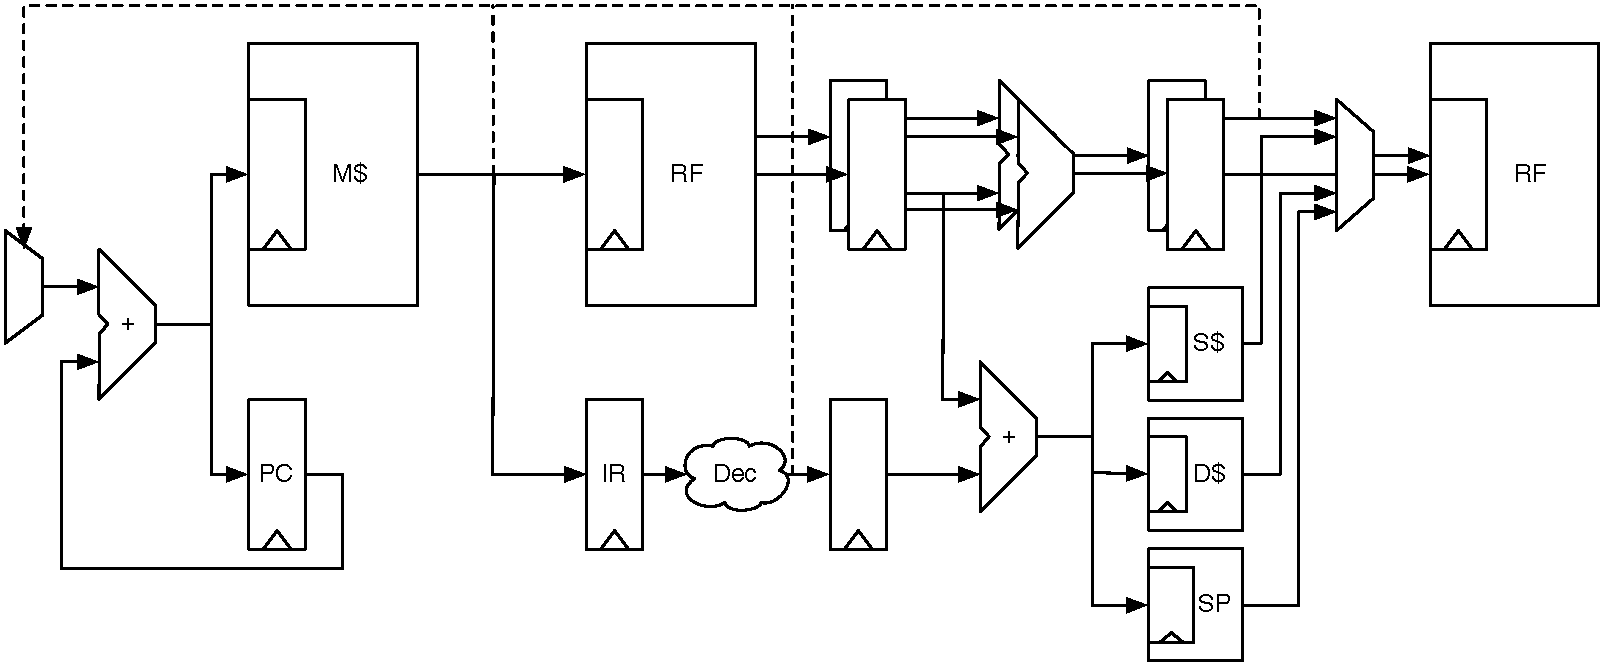
\includegraphics[width=\textwidth]{fig/pipeline}
    \caption{Pipeline of Patmos with fetch, decode, execute, memory, and write back stages.}\label{fig:pipeline}
\end{figure}

Some instructions define additional pipeline stages. Multiplication instructions
are executed, starting from the \texttt{EX} stage, in a parallel pipeline with
fixed-length (see the instruction definition). The respective stages are
referred to by \texttt{EX$_1$}, \dots, \texttt{EX$_n$}.

\martin{\todo{A more detailed description of the pipeline stages, as the individual
4 stage description is gone.} Here a start:}

\subsection{Fetch}

Fetch one or two words of instruction from the ROM or instruction cache.
Calculate next PC depending on the length of the instruction bundle.

\subsection{Decode}

Decode the instruction and generate control signals for the following stages.
Read register operands. Sign or zero extend immediate operands.

\subsection{Execute}

Read predicate registers. Conditional execute (ALU) instructions.
Write predicate register. Calculate effective address for memory operations.

\subsection{Memory}

Read or write memory. This is the only pipeline stage that might
stall the pipeline.

\subsection{Write Back}

Write result into destination register.

\stefan{Note that in the \texttt{pasim} simulator the Memory and Write Back stages are merged into a single MW stage at the time of writing,
and the stages are simulated from back to front.
While this has no effect on the timing and hazards of the instructions, there is only a single bypass from MW to EX (per pipeline). Apart
from that, all implementations of all instructions in the simulator should adhere to the above description of the stages.}

\section{Local Memories}

Patmos contains several on-chip memories, as sketched in Figure~\ref{fig:pipeline}.
We apply the idea of split caches~\cite{jop:dcache:rts} to simplify and enhance
the cache analysis. Instructions are fetched from the instruction cache.
Patmos also supports instruction and data scratchpad memories.
Stack allocated data is cached in a stack cache the other data in the
data cache with LRU replacement. Accesses to data that are hard to analyze can
bypass the data cache.

% \cite{jop:ocwcet:ccpe}



\section{Register Files}

The register files available in Patmos are depicted by
Figure~\ref{fig:registers}. In short, Patmos offers:
\begin{itemize}
  \item 32, 32-bit general-purpose registers (\texttt{R}) : \texttt{r0}, \dots, \texttt{r31} \\
    \texttt{r0} is read-only, set to zero (\texttt{0}).
  \item 8, single-bit predicate registers (\texttt{P}): \texttt{p0}, \dots, \texttt{p7}, \\
    \texttt{p0} is read-only, set to \texttt{true} (\texttt{1}).
  \item 16, 32-bit special-purpose registers (\texttt{S}): \texttt{s0}, \dots, \texttt{s15}
\end{itemize}

The general-purpose registers \texttt{R} are read in the \code{DEC} stage
and written in the \code{WB} stage. Full forwarding makes them available
in the \code{EX} stage before written into the register file.
The predicate registers are single bits that are set and read in the \code{EX}
stage.
The special registers \code{S} is just a collection of various ``special''
processor registers (e.g., stack cache pointers).
These registers might be used by different units/stages
in the pipeline and are not physically collected in a ``register file''.
The pipeline stage where those registers are read and written by the
\code{mfs} and \code{mts} are dependent on the type of the special
register.
%
\martin{The three `register' files shall constitute the state of the processor.
Every non-obvious register, such as method base, shall be mapped to a
`special' register. Even the current PC on an interrupt shall end up in a
register that is mapped into the special register domain.}
%
\stefan{Umm .. it would be really good to define somewhere in which stages which special register is actually read or written by mfs/mts
;).}
%
So all-in-all the recoverable process state is: general-purpose registers
\code{R}, the predicates \code{P}, and a collection of various processor
registers mapped to the ``special'' register file \code{S}.

Concurrently writing and reading the same register in the same cycle
will, for the read, yield the new value of the register (the register file
provides internal forwarding). Reads in
subsequent cycles return the result most recently written to the
register, i.e., the pipeline implements full forwarding.

When writing concurrently to the same register, the result is
undefined. If two instructions of the current bundle have the same
destination register, the result is only defined if the predicate of
at most one instruction in the bundle evaluates to \texttt{true} (1).

\wolf{In practice, the result is even defined if both instructions
  write to the same register, but I would not make this a feature of
  the ISA.}

The predicate registers are usually encoded as $4$-bit operands, where the most
significant bit indicates that the value read from the register file should be
inverted before it is used. For operands that are written, this additional bit
is omitted.

The special-purpose registers of \texttt{S} allow access to some dedicated
registers:
\begin{itemize}
  \item The lower $8$ bits of \texttt{s0} can be used to save/restore
    \emph{all} predicate registers at once. The other bits of that
    register are currently reserved, but not used. Setting the reserved
	bits has no effect.
  \item \texttt{s2} and \texttt{s3} can also be accessed through the names
    \texttt{sl} and \texttt{sh} and represent the lower and upper
    32-bits a multiplication.
  \item \texttt{s5} can also be accessed through the name \texttt{ss} and
    represents the register pointing to the top of the saved stack
	content in the main memory (i.e., the current stack spill pointer).
	Updating \texttt{s5} does not change \texttt{s6} or spill the stack cache.
  \item \texttt{s6} can also be accessed through the name \texttt{st} and
    represents a pointer to the top-most element of the content of the
    stack cache.
	Updating \texttt{s6} does not change \texttt{s5} or spill the stack cache.
\end{itemize}

\stefan{None of the registers should be read-only, as they need to be restored when
we switch contexts.}

\begin{figure}[p]

  \begin{multicols}{2}
    \centering

    \subfloat[\label{fig:registers:r}General-Purpose Registers (\texttt{R})]{
      \begin{bytefield}[bitwidth=.59em]{32}
        \bitheader{0-31} \\
        \bitbox{32}{r0 (zero, read-only)} \\
        \bitbox{32}{r1 (result, scratch)} \\
        \bitbox{32}{r2 (result 64-bit, scratch)} \\
        \bitbox{32}{r3 (argument 1, scratch)} \\
        \bitbox{32}{r4 (argument 2, scratch)} \\
        \bitbox{32}{r5 (argument 3, scratch)} \\
        \bitbox{32}{r6 (argument 4, scratch)} \\
        \bitbox{32}{r7 (argument 5, scratch)} \\
        \bitbox{32}{r8 (argument 6, scratch)} \\ \bitbox{32}{r9 (scratch)} \\
        \bitbox{32}{r10 (scratch)} \\ \bitbox{32}{r11 (scratch)} \\
        \bitbox{32}{r12 (scratch)} \\ \bitbox{32}{r13 (scratch)} \\
        \bitbox{32}{r14 (scratch)} \\ \bitbox{32}{r15 (scratch)} \\
        \bitbox{32}{r16 (scratch)} \\ \bitbox{32}{r17 (scratch)} \\
        \bitbox{32}{r18 (scratch)} \\ \bitbox{32}{r19 (scratch)} \\
        \bitbox{32}{r20 (scratch)} \\ \bitbox{32}{r21 (saved)} \\
        \bitbox{32}{r22 (saved)} \\ \bitbox{32}{r23 (saved)} \\
        \bitbox{32}{r24 (saved)} \\ \bitbox{32}{r25 (saved)} \\
        \bitbox{32}{r26 (saved)} \\ \bitbox{32}{r27 (saved)} \\
        \bitbox{32}{r28 (saved)} \\
        \bitbox{32}{r29 (temp.\ register, saved)} \\
        \bitbox{32}{r30 (frame pointer, saved)} \\
        \bitbox{32}{r31 (stack pointer, saved)} \\
      \end{bytefield}
    }

    \newpage

    \vspace*{\stretch{1}}

    \subfloat[\label{fig:registers:pr}Predicate Registers (\texttt{P})]{
      \newcommand{\bitlabel}[1]{
        \bitbox[]{1}{\raisebox{0pt}[5ex][1pt]{\turnbox{45}{\fontsize{7}{7}\selectfont#1}}}
      }
      \begin{bytefield}[bitwidth=1.5em]{8}
        \bitlabel{p7} \bitlabel{p6} \bitlabel{p5} \bitlabel{p4}
        \bitlabel{p3} \bitlabel{p2} \bitlabel{p1} \bitlabel{p0 -- Read only, always \texttt{1}} \\
        \bitheader{0-7} \\
        \bitbox{1}{} \bitbox{1}{} \bitbox{1}{} \bitbox{1}{}
        \bitbox{1}{} \bitbox{1}{} \bitbox{1}{} \bitbox{1}{} \\
      \end{bytefield}
    }

    \vspace*{\stretch{2}}

    \subfloat[\label{fig:registers:s}Special-Purpose Registers (\texttt{S})]{
      \begin{bytefield}[bitwidth=.59em]{32}
        \bitheader{0-31} \\
        \bitbox{24}{reserved} \bitbox{8}{p7 \dots p0} \bitbox[]{4}{s0} \\
        \bitbox{32}{s1} \\
        \bitbox{32}{sl (mul low)} \bitbox[]{4}{s2} \\
        \bitbox{32}{sh (mul high)} \bitbox[]{4}{s3} \\
        \bitbox{32}{s4} \\
        \bitbox{32}{ss (spill pointer)} \bitbox[]{4}{s5} \\
        \bitbox{32}{st (stack pointer)} \bitbox[]{4}{s6} \\
        \bitbox{32}{srb (return base)} \bitbox[]{4}{s7} \\
        \bitbox{32}{sro (return offset)} \bitbox[]{4}{s8} \\
        \bitbox{32}{sxb (exception return base)} \bitbox[]{4}{s9} \\
        \bitbox{32}{sxo (exception return offset)} \bitbox[]{4}{s10} \\
        \bitbox{32}{s11} \\
        \bitbox{32}{s12} \\ \bitbox{32}{s13} \\ \bitbox{32}{s14} \\ \bitbox{32}{s15} \\
      \end{bytefield}
    }

    \vspace*{\stretch{4}}~

  \end{multicols}

  \caption{General-purpose register file, predicate registers, and
           special-purpose registers of Patmos.}
  \label{fig:registers}
\end{figure}

\section{Bundle Formats}

All Patmos instructions are 32 bits wide and are structured according to
one of the instruction formats defined in the following section. Up to two
instructions can be combined to form an instruction bundle; Patmos bundles are
thus either 32 or 64 bits wide. The bundles sizes are recognized by the value of
the most significant bit, where $0$ indicates a short, 32-bit bundle and $1$ a
long, 64-bit bundle.

The following figures illustrate these two bundle variants:
\begin{itemize}
 \item 32-bit bundle format\\[2ex]
   \begin{bytefield}{32}
     \bitheader{0-31} \\
     \bitbox{1}{0} & \bitbox{31}{\bitssubclass} \\
   \end{bytefield}

 \item 64-bit bundle format \\[2ex]
   \begin{bytefield}[lsb=32]{32} \bitheader{32-63} \\
     \bitbox{1}{1} & \bitbox{31}{\bitssubclass} \\
   \end{bytefield}
   \hspace{.5em}
   \begin{bytefield}{32} \bitheader{0-31} \\
     \bitbox{1}{x} & \bitbox{31}{\bitssubclass} \\
   \end{bytefield}
\end{itemize}

\section{Instruction Formats}

This section gives an overview of all instruction formats defined in the Patmos
ISA. Individual instructions of the various formats are defined in the next
section. Gray fields indicate bits whose function is determined by a sub-class
of the instruction format. Black fields are not used.

\begin{itemize}
  \item AluImm -- Arithmetic Immediate (ALUi) \\[2ex]
    \begin{bytefield}{32}
      \bitheader{0-31} \\
      \bitbox{1}{x} & \bitbox{4}{Pred} & \bitbox{2}{00} & \bitbox{3}{Func} &
      \bitbox{5}{Rd} & \bitbox{5}{Rs1} & \bitbox{12}{Immediate} \\
    \end{bytefield}
  \item AluLongImm -- Long Immediate (ALUl) \\[2ex]
    \begin{bytefield}{32}
      \bitheader{0-31} \\
      \bitbox{1}{1} & \bitbox{4}{Pred} & \bitbox{5}{11111} &
      \bitbox{5}{Rd} & \bitbox{5}{Rs1} & \bitbox{5}{\bitsunused} &
      \bitbox{3}{000} & \bitbox{4}{Func} \\
      \bitheader{0-31} \\
      \bitbox{32}{Long Immediate} \\
    \end{bytefield}
  \item Alu -- Arithmetic (ALU) \\[2ex]
        \begin{bytefield}{32}
          \bitheader{0-31} \\
          \bitbox{1}{x} & \bitbox{4}{Pred} & \bitbox{5}{01000} &
          \bitbox{15}{\bitssubclass} &
          \bitbox{3}{Opc} & \bitbox{4}{Func} \\
        \end{bytefield}

        \begin{bytefield}[leftcurly=.]{32}
          \begin{leftwordgroup}{\parbox{8em}{AluReg -- Register (ALUr)}}
            \bitheader{0-31} \\
            \bitbox{1}{x} & \bitbox{4}{Pred} & \bitbox{5}{01000} &
            \bitbox{5}{Rd} & \bitbox{5}{Rs1} & \bitbox{5}{Rs2} &
            \bitbox{3}{000} & \bitbox{4}{Func}
          \end{leftwordgroup} \\
          \begin{leftwordgroup}{\parbox{8em}{ALUm -- Multiply}}
            \bitheader{0-31} \\
            \bitbox{1}{x} & \bitbox{4}{Pred} & \bitbox{5}{01000} &
            \bitbox{5}{\bitsunused} & \bitbox{5}{Rs1} & \bitbox{5}{Rs2} &
            \bitbox{3}{010} & \bitbox{4}{Func}
          \end{leftwordgroup} \\
          \begin{leftwordgroup}{\parbox{8em}{ALUc -- Compare}}
            \bitheader{0-31} \\
            \bitbox{1}{x} & \bitbox{4}{Pred} & \bitbox{5}{01000} &
            \bitbox{2}{\bitsunused} & \bitbox{3}{Pd} & \bitbox{5}{Rs1} & \bitbox{5}{Rs2} &
            \bitbox{3}{011} & \bitbox{4}{Func}
          \end{leftwordgroup} \\
          \begin{leftwordgroup}{\parbox{8em}{ALUp -- Predicate}}
            \bitheader{0-31} \\
            \bitbox{1}{x} & \bitbox{4}{Pred} & \bitbox{5}{01000} &
            \bitbox{2}{\bitsunused} & \bitbox{3}{Pd} & \bitbox{1}{\bitsunused} & \bitbox{4}{Ps1} & \bitbox{1}{\bitsunused} & \bitbox{4}{Ps2} &
            \bitbox{3}{100} & \bitbox{4}{Func}
          \end{leftwordgroup} \\
          \begin{leftwordgroup}{\parbox{8em}{ALUb -- Bitcopy}}
            \bitheader{0-31} \\
            \bitbox{1}{x} & \bitbox{4}{Pred} & \bitbox{5}{01000} &
            \bitbox{5}{Rd} & \bitbox{5}{Rs1} & \bitbox{5}{Imm} &
            \bitbox{3}{101} & \bitbox{4}{Ps}
          \end{leftwordgroup} \\
          \begin{leftwordgroup}{\parbox{8em}{ALUci -- Compare immediate}}
            \bitheader{0-31} \\
            \bitbox{1}{x} & \bitbox{4}{Pred} & \bitbox{5}{01000} &
            \bitbox{2}{\bitsunused} & \bitbox{3}{Pd} & \bitbox{5}{Rs1} & \bitbox{5}{Imm} &
            \bitbox{3}{110} & \bitbox{4}{Func}
          \end{leftwordgroup} \\
          %% \begin{leftwordgroup}{\parbox{8em}{Unused}}
          %%   \bitheader{0-31} \\
          %%   \bitbox{1}{x} & \bitbox{4}{Pred} & \bitbox{5}{01000} &
          %%   \bitbox{15}{\bitssubclass} &
          %%   \bitbox{3}{111} & \bitbox{4}{Func}
          %% \end{leftwordgroup} \\
        \end{bytefield}

  \item SPC -- Special \\[2ex]
        \begin{bytefield}{32}
          \bitheader{0-31} \\
          \bitbox{1}{x} & \bitbox{4}{Pred} & \bitbox{5}{01001} &
          \bitbox{15}{\bitssubclass} &
          \bitbox{3}{Opc} & \bitbox{4}{I/R/F} \\
        \end{bytefield}

        \begin{bytefield}[leftcurly=.]{32}
          \begin{leftwordgroup}{\parbox{11em}{SPCt -- Move To Special}}
            \bitheader{0-31} \\
            \bitbox{1}{x} & \bitbox{4}{Pred} & \bitbox{5}{01001} &
            \bitbox{5}{\bitsunused} & \bitbox{5}{Rs1} & \bitbox{5}{\bitsunused} &
            \bitbox{3}{010} & \bitbox{4}{Sd}
          \end{leftwordgroup} \\
          \begin{leftwordgroup}{\parbox{11em}{SPCf -- Move From Special}}
            \bitheader{0-31} \\
            \bitbox{1}{x} & \bitbox{4}{Pred} & \bitbox{5}{01001} &
            \bitbox{5}{Rd} & \bitbox{10}{\bitsunused} &
            \bitbox{3}{011} & \bitbox{4}{Ss}
          \end{leftwordgroup} \\
          %% \begin{leftwordgroup}{\parbox{11em}{Unused}}
          %%   \bitheader{0-31} \\
          %%   \bitbox{1}{x} & \bitbox{4}{Pred} & \bitbox{5}{01001} &
          %%   \bitbox{15}{\bitssubclass} &
          %%   \bitbox{3}{000} & \bitbox{4}{I/R/F}
          %% \end{leftwordgroup} \\
          %% \begin{leftwordgroup}{\parbox{11em}{Unused}}
          %%   \bitheader{0-31} \\
          %%   \bitbox{1}{x} & \bitbox{4}{Pred} & \bitbox{5}{01001} &
          %%   \bitbox{15}{\bitssubclass} &
          %%   \bitbox{3}{100} & \bitbox{4}{I/R/F}
          %% \end{leftwordgroup} \\
          %% \begin{leftwordgroup}{\parbox{11em}{Unused}}
          %%   \bitheader{0-31} \\
          %%   \bitbox{1}{x} & \bitbox{4}{Pred} & \bitbox{5}{01001} &
          %%   \bitbox{15}{\bitssubclass} &
          %%   \bitbox{3}{101} & \bitbox{4}{I/R/F}
          %% \end{leftwordgroup} \\
          %% \begin{leftwordgroup}{\parbox{11em}{Unused}}
          %%   \bitheader{0-31} \\
          %%   \bitbox{1}{x} & \bitbox{4}{Pred} & \bitbox{5}{01001} &
          %%   \bitbox{15}{\bitssubclass} &
          %%   \bitbox{3}{110} & \bitbox{4}{I/R/F}
          %% \end{leftwordgroup} \\
          %% \begin{leftwordgroup}{\parbox{11em}{Unused}}
          %%   \bitheader{0-31} \\
          %%   \bitbox{1}{x} & \bitbox{4}{Pred} & \bitbox{5}{01001} &
          %%   \bitbox{15}{\bitssubclass} &
          %%   \bitbox{3}{111} & \bitbox{4}{I/R/F}
          %% \end{leftwordgroup}
        \end{bytefield}

  \item LDT -- Load Typed \\[2ex]
        \begin{bytefield}{32}
          \bitheader{0-31} \\
          \bitbox{1}{x} & \bitbox{4}{Pred} & \bitbox{5}{01010} &
          \bitbox{5}{Rd} & \bitbox{5}{Ra} & \bitbox{5}{Type} & \bitbox{7}{Offset} \\
        \end{bytefield}
  \item STT -- Store Typed \\[2ex]
        \begin{bytefield}{32}
          \bitheader{0-31} \\
          \bitbox{1}{x} & \bitbox{4}{Pred} & \bitbox{5}{01011} &
          \bitbox{5}{Type} & \bitbox{5}{Ra} & \bitbox{5}{Rs} & \bitbox{7}{Offset} \\
        \end{bytefield}

  \item STC -- Stack Control \\[2ex]
        \begin{bytefield}{32}
          \bitheader{0-31} \\
          \bitbox{1}{x} & \bitbox{4}{Pred} & \bitbox{5}{01100} &
          \bitbox{2}{Op} & \bitbox{2}{F} & \bitbox{18}{\bitssubclass} \\
        \end{bytefield}

        \begin{bytefield}[leftcurly=.]{32}
          \begin{leftwordgroup}{\parbox{13em}{STCi -- Stack Control Immediate}}
            \bitheader{0-31} \\
            \bitbox{1}{x} & \bitbox{4}{Pred} & \bitbox{5}{01100} &
            \bitbox{2}{Op} & \bitbox{2}{00} &
            \bitbox{18}{Immediate}
          \end{leftwordgroup} \\
          \begin{leftwordgroup}{\parbox{13em}{STCr -- Stack Control Register}}
            \bitheader{0-31} \\
            \bitbox{1}{x} & \bitbox{4}{Pred} & \bitbox{5}{01100} &
            \bitbox{2}{Op} & \bitbox{2}{01} &
            \bitbox{1}{\bitsunused} & \bitbox{5}{Rs} & \bitbox{12}{\bitsunused}
          \end{leftwordgroup}
        \end{bytefield}

  \item CFLi -- Control Flow with Immediate \nopagebreak\\[2ex]
        \begin{bytefield}{32}
          \bitheader{0-31} \\
          \bitbox{1}{x} & \bitbox{4}{Pred} & \bitbox{2}{10} & \bitbox{2}{Op} & \bitbox{1}{d} &
          \bitbox{22}{Immediate} \\
        \end{bytefield}

  \item CFLr -- Control Flow with Registers \\[2ex]
        \begin{bytefield}{32}
          \bitheader{0-31} \\
          \bitbox{1}{x} & \bitbox{4}{Pred} & \bitbox{4}{1100} & \bitbox{1}{d} &
          \bitbox{18}{\bitssubclass} & \bitbox{2}{F} & \bitbox{2}{Op} \\
        \end{bytefield}

        \begin{bytefield}[leftcurly=.]{32}
          \begin{leftwordgroup}{\parbox{18em}{CFLri -- Control Flow with implicit registers}}
          \bitheader{0-31} \\
          \bitbox{1}{x} & \bitbox{4}{Pred} & \bitbox{4}{1100} & \bitbox{1}{d} &
          \bitbox{18}{\bitsunused} &
          \bitbox{2}{00} & \bitbox{2}{Op}
          \end{leftwordgroup}\\
          \begin{leftwordgroup}{\parbox{18em}{CFLrs -- Control Flow with single register}}
          \bitheader{0-31} \\
          \bitbox{1}{x} & \bitbox{4}{Pred} & \bitbox{4}{1100} & \bitbox{1}{d} &
          \bitbox{5}{\bitsunused} & \bitbox{5}{Rs} & \bitbox{8}{\bitsunused} &
          \bitbox{2}{01} & \bitbox{2}{Op}
          \end{leftwordgroup}\\
          \begin{leftwordgroup}{\parbox{18em}{CFLrt -- Control Flow with two registers}}
          \bitheader{0-31} \\
          \bitbox{1}{x} & \bitbox{4}{Pred} & \bitbox{4}{1100} & \bitbox{1}{d} &
          \bitbox{5}{\bitsunused} & \bitbox{5}{Rs1} & \bitbox{5}{Rs2} & \bitbox{3}{\bitsunused} &
          \bitbox{2}{10} & \bitbox{2}{Op}
          \end{leftwordgroup}
        \end{bytefield}
\end{itemize}

\clearpage
\section{Instruction Opcodes}
\label{sec:instruction_opcodes}

This section defines the instruction set architecture, the instruction opcodes,
and the behavior of the respective instructions of Patmos.

\subsection{Binary Arithmetic}

Applies to the AluReg, AluImm, and AluLongImm formats.  Operand \texttt{Op2}
denotes either the \texttt{Rs2}, or the \texttt{Immediate} operand, or
the \texttt{Long Immediate}. The immediate operand is zero-extended.  For
shift and rotate operations, only the lower 5 bits of the operand
are considered. Table~\ref{tab:alufunc} shows the encoding of the
\texttt{func} field; for AluImm instructions, only functions in the
upper half of that table are available.

\begin{itemize}
  \item AluReg -- Register (ALUr) \\[2ex]
    \begin{bytefield}{32}
      \bitheader{0-31} \\
      \bitbox{1}{x} & \bitbox{4}{Pred} & \bitbox{5}{01000} &
      \bitbox{5}{Rd} & \bitbox{5}{Rs1} & \bitbox{5}{Rs2} &
      \bitbox{3}{000} & \bitbox{4}{Func} \\
    \end{bytefield}
  \item AluImm -- Arithmetic Immediate (ALUi) \\[2ex]
    \begin{bytefield}{32}
      \bitheader{0-31} \\
      \bitbox{1}{x} & \bitbox{4}{Pred} & \bitbox{2}{00} & \bitbox{3}{Func} &
      \bitbox{5}{Rd} & \bitbox{5}{Rs1} & \bitbox{12}{Immediate} \\
    \end{bytefield}
  \item AluLongImm -- Long Immediate (ALUl)\\[2ex]
    \begin{bytefield}{32}
      \bitheader{0-31} \\
      \bitbox{1}{1} & \bitbox{4}{Pred} & \bitbox{5}{11111} &
      \bitbox{5}{Rd} & \bitbox{5}{Rs1} & \bitbox{5}{\bitsunused} &
      \bitbox{3}{000} & \bitbox{4}{Func} \\
      \bitheader{0-31} \\
      \bitbox{32}{Long Immediate} \\
   \end{bytefield}
\end{itemize}

\begin{table}[hb]
  \centering
  \begin{tabular}{lll}
    \toprule
    Func & Name   & Semantics \\
    \midrule
    0000 & add    & \texttt{Rd = Rs1 + Op2} \\
    0001 & sub    & \texttt{Rd = Rs1 - Op2} \\
    0010 & xor    & \texttt{Rd = Rs1 \XOR Op2} \\
    0011 & sl     & \texttt{Rd = Rs1 \shl Op2$_{(4:0)}$} \\
    0100 & sr     & \texttt{Rd = Rs1 \shr Op2$_{(4:0)}$} \\
    0101 & sra    & \texttt{Rd = Rs1 \ashr Op2$_{(4:0)}$} \\
    0110 & or     & \texttt{Rd = Rs1 \OR Op2} \\
    0111 & and    & \texttt{Rd = Rs1 \AND Op2} \\
    \cmidrule{1-3}
    1000 & ---	& unused \\
    1001 & ---    & unused \\
    1010 & ---    & unused \\
    1011 & nor    & \texttt{Rd = \NOT (Rs1 \OR Op2)} \\
    1100 & shadd  & \texttt{Rd = (Rs1 \shl 1) + Op2} \\
    1101 & shadd2 & \texttt{Rd = (Rs1 \shl 2) + Op2} \\
    1110 & ---    & unused \\
    1111 & ---    & unused \\
    \bottomrule
  \end{tabular}
  \caption{General ALU functions}
  \label{tab:alufunc}
\end{table}

\paragraph{Pseudo Instructions}
\begin{itemize}
  \item \texttt{mov Rd = Rs}~\dots~\texttt{add Rd = Rs + 0}
  \item \texttt{clr Rd}~\dots~\texttt{add Rd = r0 + 0}
  \item \texttt{neg Rd = -Rs}~\dots~\texttt{sub Rd = 0 - Rs}
  \item \texttt{not Rd = \NOT Rs}~\dots~\texttt{nor Rd = \NOT (Rs \OR R0)}
  \item \texttt{li Rd = Immediate}~\dots~\texttt{add Rd = r0 + Immediate}
  \item \texttt{li Rd = Immediate}~\dots~\texttt{sub Rd = r0 - Immediate}
  \item \texttt{nop}~\dots~\texttt{sub r0 = r0 - 0}
\end{itemize}


\paragraph{Note}
The use of \texttt{sub r0 = r0 - 0} to encode a \texttt{nop}
pseudo-instruction results in a value of \texttt{0x00400000} in the
binary instruction stream. This helps in distinguishing the execution
of compiler-generated \texttt{nops} from executing instructions from
memory that happens to be zero.

\clearpage
\subsection{Multiply}

Applies to the ALUm format only. Multiplications are executed in
parallel with the regular pipeline and finish within a fixed number of
cycles \todo{how many?}. Table~\ref{tab:mulfunc} shows the encoding of
the \texttt{func} field for the ALUm instruction format.

\begin{itemize}
  \item ALUm -- Multiply \\[2ex]
    \begin{bytefield}{32}
      \bitheader{0-31} \\
      \bitbox{1}{x} & \bitbox{4}{Pred} & \bitbox{5}{01000} &
      \bitbox{5}{\bitsunused} & \bitbox{5}{Rs1} & \bitbox{5}{Rs2} &
      \bitbox{3}{010} & \bitbox{4}{Func} \\
    \end{bytefield}
\end{itemize}

\begin{table}[hb]
  \centering
  \begin{tabular}{lll}
    \toprule
    Func & Name   & Semantics \\
    \midrule
    0000 & mul    & \texttt{sl = Rs1 * Rs2;}\\
         &        & \texttt{sh = (Rs1 * Rs2) \shr 32} \\
    0001 & mulu   & \texttt{sl = (uint32\_t)Rs1 * (uint32\_t)Rs2;} \\
         &        & \texttt{sh = ((uint32\_t)Rs1 * (uint32\_t)Rs2) \shr 32} \\
    0010 & ---    & unused \\
    \dots& \dots  & \dots \\
    1111 & ---    & unused \\
    \bottomrule
  \end{tabular}
  \caption{Multiplication functions}
  \label{tab:mulfunc}
\end{table}


\paragraph{Behavior}

Perform multiplication in multiple cycles and write the result into
destination registers \texttt{sl} and \texttt{sh}.

\paragraph{Note}

Multiplications are pipelined, it is thus possible to issue one multiplication on
every clock cycle. Multiplications can only be issued in the first slot.

\stefan{Not yet final. 64bit support and the special registers for multiply might
vanish. Maybe merge mul and mulu into the ALU Func field somehow to kill off the ALUm format?
We could keep the special register to access the high word and write the low
word into a GPR when using ALUl format, so we save one mfs per mul.
(remove this comment when multiply ISA is (somewhat) finalized)}

\clearpage
\subsection{Compare}

Applies to the ALUc and ALUci formats only. Operand \texttt{Op2}
denotes either the \texttt{Rs2}, or the \texttt{Imm}
operand. Tables~\ref{tab:cmpfunc} show the encoding of the
\texttt{func} field for the ALUc and ALUci formats.

\begin{itemize}
  \item ALUc -- Compare \\[2ex]
    \begin{bytefield}{32}
      \bitheader{0-31} \\
      \bitbox{1}{x} & \bitbox{4}{Pred} & \bitbox{5}{01000} &
      \bitbox{2}{\bitsunused} & \bitbox{3}{Pd} & \bitbox{5}{Rs1} & \bitbox{5}{Rs2} &
      \bitbox{3}{011} & \bitbox{4}{Func} \\
    \end{bytefield}
  \item ALUci -- Compare immediate \\[2ex]
    \begin{bytefield}{32}
      \bitheader{0-31} \\
      \bitbox{1}{x} & \bitbox{4}{Pred} & \bitbox{5}{01000} &
      \bitbox{2}{\bitsunused} & \bitbox{3}{Pd} & \bitbox{5}{Rs1} & \bitbox{5}{Imm} &
      \bitbox{3}{110} & \bitbox{4}{Func} \\
    \end{bytefield}
\end{itemize}

\begin{table}[hb]
  \centering
  \begin{tabular}{lll}
    \toprule
    Func & Name   & Semantics \\
    \midrule
    0000 & cmpeq  & \texttt{Pd = Rs1 ==  Op2} \\
    0001 & cmpneq & \texttt{Pd = Rs1 !=  Op2} \\
    0010 & cmplt  & \texttt{Pd = Rs1 \textless\ Op2} \\
    0011 & cmple  & \texttt{Pd = Rs1 \textless= Op2} \\
    0100 & cmpult & \texttt{Pd = Rs1 \textless\ Op2, unsigned} \\
    0101 & cmpule & \texttt{Pd = Rs1 \textless= Op2, unsigned} \\
    0110 & btest  & \texttt{Pd = (Rs1 \AND (1 \shl Op2)) != 0} \\
    0111 & ---    & unused \\
    \dots& \dots  & \dots \\
    1111 & ---    & unused \\
    \bottomrule
  \end{tabular}
  \caption{Compare functions}
  \label{tab:cmpfunc}
\end{table}

\paragraph{Pseudo Instructions}
\begin{itemize}
  \item \texttt{isodd Pd = Rs1}~\dots~\texttt{btest Pd = Rs1[r0]}
  \item \texttt{mov Pd = Rs}~\dots~\texttt{cmpneq Pd = Rs != r0}
\end{itemize}

\paragraph{Note}

The predicate register is read and written in the execute stage.

\stefan{We discussed about adding short immediate versions, but with the current predicate handling this is not
a trivial change for the compiler, so we skip that. Instead, we might introduce bez/bnez instructions, which is much more common anyway.}

\clearpage
\subsection{Predicate}

Applies to the ALUp format only, the opcodes correspond to those of
the ALU operations on general purpose
registers. Table~\ref{tab:predfunc} shows the encoding of the
\texttt{func} field for the ALUp format.

\martin{Why do we have this encoding of predicate operations with empty function
codes in-between? No need to be `compatible' with ALU operations, just makes decoding
a little bit more complex.}

\begin{itemize}
  \item ALUp -- Predicate \\[2ex]
    \begin{bytefield}{32}
      \bitheader{0-31} \\
      \bitbox{1}{x} & \bitbox{4}{Pred} & \bitbox{5}{01000} &
      \bitbox{2}{\bitsunused} & \bitbox{3}{Pd} & \bitbox{1}{\bitsunused} & \bitbox{4}{Ps1} & \bitbox{1}{\bitsunused} & \bitbox{4}{Ps2} &
      \bitbox{3}{100} & \bitbox{4}{Func} \\
    \end{bytefield}
\end{itemize}

\begin{table}[hb]
  \centering
  \begin{tabular}{lll}
    \toprule
    Func & Name   & Semantics \\
    \midrule
    0000 & ---    & unused \\
    \dots& \dots  & \dots \\
    0101 & ---    & unused \\
    0110 & por     & \texttt{Pd = Ps1 \OR Ps2} \\
    0111 & pand    & \texttt{Pd = Ps1 \AND Ps2} \\
    1000 & ---    & unused \\
    1001 & ---    & unused \\
    1010 & pxor    & \texttt{Pd = Ps1 \XOR Ps2} \\
    1011 & ---    & unused \\
    \dots& \dots  & \dots \\
    1111 & ---    & unused \\
    \bottomrule
  \end{tabular}
  \caption{Predicate functions}
  \label{tab:predfunc}
\end{table}

\paragraph{Pseudo Instructions}
\begin{itemize}
  \item \texttt{pmov Pd = Ps}~\dots~\texttt{por Pd = Ps \OR Ps}
  \item \texttt{pnot Pd = \NOT Ps}~\dots~\texttt{pxor Pd = (Ps \XOR p0)}
  \item \texttt{pset Pd = 1}~\dots~\texttt{por Pd = p0 \OR p0}
  \item \texttt{pclr Pd = 0}~\dots~\texttt{pxor Pd = p0 \XOR p0}
\end{itemize}

\paragraph{Note}
The predicate register is read and written in the execute stage.
All predicate combine instruction mnemonics (including pseudo instructions) are prefixed with \texttt{p},
all other instructions involving predicates are not prefixed (e.g., moving from register to predicate).

\stefan{We have a mov with two registers (\texttt{add}), mov with two predicates (\texttt{por}), a mov from register to
predicate (\texttt{cmpnez}), as well as mov from register bit to predicate (\texttt{btest}), but we are missing a
mov from predicate to register (is now a predicated set and predicated clr), and mov from predicate to register bit (is now done with
bitmasks).}

\clearpage
\subsection{Bitcopy}

Applies to the ALUb format only. The only instruction with this
encoding is \texttt{bcopy}, which is the ``inverse'' of the
\code{btest} instruction. It has the following semantics: \texttt{Rd =
  (Rs1 \AND \NOT (1 \shl Imm)) \OR (Ps \shl Imm)}\\
Note that operand \texttt{Ps}, like the source operands in the ALUp format,
can be inverted.

\begin{itemize}
  \item ALUb -- Bitcopy \\[2ex]
    \begin{bytefield}{32}
      \bitheader{0-31} \\
      \bitbox{1}{x} & \bitbox{4}{Pred} & \bitbox{5}{01000} &
      \bitbox{5}{Rd} & \bitbox{5}{Rs1} & \bitbox{5}{Imm} &
      \bitbox{3}{101} & \bitbox{4}{Ps} \\
    \end{bytefield}
\end{itemize}

\paragraph{Pseudo Instructions}
\begin{itemize}
  \item \texttt{mov Rd = Ps}~\dots~\texttt{bcopy Rd = r0, 0, Ps}
\end{itemize}

\paragraph{Note}
The predicate register is read in the execute stage.

\clearpage
\subsection{Move To Special}

Applies to the SPCt format only. Copy the value of a general-purpose
register to a special-purpose register. The only instruction is
\texttt{mts}, which stores the content of general-purpose register
\texttt{Rs1} in special register \texttt{Sd}.

\begin{itemize}
  \item SPCt -- Move To Special \\[2ex]
    \begin{bytefield}{32}
      \bitheader{0-31} \\
      \bitbox{1}{x} & \bitbox{4}{Pred} & \bitbox{5}{01001} &
      \bitbox{5}{\bitsunused} & \bitbox{5}{Rs1} & \bitbox{5}{\bitsunused} &
      \bitbox{3}{010} & \bitbox{4}{Sd} \\
    \end{bytefield}
\end{itemize}



\paragraph{Note}

\martin{\todo{We should document in which stage each special register
is read and written.}}

\clearpage
\subsection{Move From Special}

Applies to the SPCf format only. Copy the value of a special-purpose
register to a general-purpose register. The only instruction is
\texttt{mfs}, which loads the content of special register \texttt{Ss}
to general-purpose register \texttt{Rd}.

\begin{itemize}
  \item SPCf -- Move From Special \\[2ex]
    \begin{bytefield}{32}
      \bitheader{0-31} \\
      \bitbox{1}{x} & \bitbox{4}{Pred} & \bitbox{5}{01001} &
      \bitbox{5}{Rd} & \bitbox{10}{\bitsunused} &
      \bitbox{3}{011} & \bitbox{4}{Ss} \\
    \end{bytefield}
\end{itemize}

\clearpage
\subsection{Load Typed}
\label{subsec:load_typed}

Applies to the LDT format only. Load from a memory or
cache. In the table accesses to the stack cache are denoted by \texttt{sc}, to
the local scratchpad memory by \texttt{lm}, to the data cache by \texttt{dc},
and to the global shared memory by \texttt{gm}. All load variants are
considered to stall until the memory access is completed.

Loads incur a load-to-use latency that has to be respected by
the compiler/programmer. The result of the load is not available in
the bundle immediately after the load, i.e., there must be one bundle
between the load instruction and the first use of the destination
register. The value of the destination register is undefined during
this load delay slot.

The displacement value (\code{Imm}) value is interpreted unsigned.

\begin{itemize}
  \item LDT -- Load Typed \\[2ex]
    \begin{bytefield}{32}
      \bitheader{0-31} \\
      \bitbox{1}{x} & \bitbox{4}{Pred} & \bitbox{5}{01010} &
      \bitbox{5}{Rd} & \bitbox{5}{Ra} & \bitbox{5}{Type} & \bitbox{7}{Immediate} \\
    \end{bytefield}
\end{itemize}

\begin{table}[htb!]
  \centering
\begin{tabular}{lll}
  \toprule
  Type            & Name   & Semantics \\
  \midrule
  000 \textbar~00 & lws    & \texttt{Rd=sc[Ra+(Imm \shl 2)]$_{32}$} \\
  000 \textbar~01 & lwl    & \texttt{Rd=lm[Ra+(Imm \shl 2)]$_{32}$ } \\
  000 \textbar~10 & lwc    & \texttt{Rd=dc[Ra+(Imm \shl 2)]$_{32}$} \\
  000 \textbar~11 & lwm    & \texttt{Rd=gm[Ra+(Imm \shl 2)]$_{32}$} \\
  001 \textbar~00 & lhs    & \texttt{Rd=(int32\_t)sc[Ra+(Imm \shl 1)]$_{16}$} \\
  001 \textbar~01 & lhl    & \texttt{Rd=(int32\_t)lm[Ra+(Imm \shl 1)]$_{16}$ } \\
  001 \textbar~10 & lhc    & \texttt{Rd=(int32\_t)dc[Ra+(Imm \shl 1)]$_{16}$} \\
  001 \textbar~11 & lhm    & \texttt{Rd=(int32\_t)gm[Ra+(Imm \shl 1)]$_{16}$} \\
  010 \textbar~00 & lbs    & \texttt{Rd=(int32\_t)sc[Ra+Imm]$_{8}$} \\
  010 \textbar~01 & lbl    & \texttt{Rd=(int32\_t)lm[Ra+Imm]$_{8}$ } \\
  010 \textbar~10 & lbc    & \texttt{Rd=(int32\_t)dc[Ra+Imm]$_{8}$} \\
  010 \textbar~11 & lbm    & \texttt{Rd=(int32\_t)gm[Ra+Imm]$_{8}$} \\
  011 \textbar~00 & lhus   & \texttt{Rd=(uint32\_t)sc[Ra+(Imm \shl 1)]$_{16}$} \\
  011 \textbar~01 & lhul   & \texttt{Rd=(uint32\_t)lm[Ra+(Imm \shl 1)]$_{16}$ } \\
  011 \textbar~10 & lhuc   & \texttt{Rd=(uint32\_t)dc[Ra+(Imm \shl 1)]$_{16}$} \\
  011 \textbar~11 & lhum   & \texttt{Rd=(uint32\_t)gm[Ra+(Imm \shl 1)]$_{16}$} \\
  100 \textbar~00 & lbus   & \texttt{Rd=(uint32\_t)sc[Ra+Imm]$_{8}$} \\
  100 \textbar~01 & lbul   & \texttt{Rd=(uint32\_t)lm[Ra+Imm]$_{8}$ } \\
  100 \textbar~10 & lbuc   & \texttt{Rd=(uint32\_t)dc[Ra+Imm]$_{8}$} \\
  100 \textbar~11 & lbum   & \texttt{Rd=(uint32\_t)gm[Ra+Imm]$_{8}$} \\
  \cmidrule{1-3}
  101 \textbar~00 & --- & unused \\
  \dots & \dots & \dots \\
  111 \textbar~11 & --- & unused \\
  \bottomrule
\end{tabular}
\caption{Typed loads}
\label{tab:loads}
\end{table}


\martin{I don't think that (uint32\_t) does the zero extension. But I might be wrong
as my C knowledge is rusty. We should use the H\&P MIPS green card notion.}



\martin{Do we do a memory read even when the predicate is false?
Some memory locations (I/O) might have side effects on a read.
Therefore, we shall not read when the predicate is false.}



\paragraph{Note}

All loads can only be issued on the first slot.

\clearpage
\subsection{Store Typed} Applies to the STT format only. Store to a memory or
cache. In the table accesses to the stack cache are denoted by \texttt{sc}, to
the local scratchpad memory by \texttt{lm}, to the data cache by \texttt{dc},
and to the global shared memory by \texttt{gm}.

\martin{TODO: make is clear at some point that \code{gm} is basically
data cache bypass. Would be natural for I/O, but mapping I/O to \code{lm},
as it is currently in passim, is also fine.}

The displacement value (\code{Imm}) value is interpreted unsigned.
Stores can only be issued on the first slot.

\begin{itemize}
  \item STT -- Store Typed \\[2ex]
    \begin{bytefield}{32}
      \bitheader{0-31} \\
      \bitbox{1}{x} & \bitbox{4}{Pred} & \bitbox{5}{01011} &
      \bitbox{5}{Type} & \bitbox{5}{Ra} & \bitbox{5}{Rs} & \bitbox{7}{Offset} \\
    \end{bytefield}
\end{itemize}

\begin{table}[hb]
  \centering
\begin{tabular}{lll}
  \toprule
  Type            & Name   & Semantics \\
  \midrule
  000 \textbar~00 & sws    & \texttt{sc[Ra+(Imm \shl 2)]$_{32}$ = Rs} \\
  000 \textbar~01 & swl    & \texttt{lm[Ra+(Imm \shl 2)]$_{32}$ = Rs} \\
  000 \textbar~10 & swc    & \texttt{dc[Ra+(Imm \shl 2)]$_{32}$ = Rs} \\
  000 \textbar~11 & swm    & \texttt{gm[Ra+(Imm \shl 2)]$_{32}$ = Rs} \\
  001 \textbar~00 & shs    & \texttt{sc[Ra+(Imm \shl 1)]$_{16}$ = Rs$_{[15:0]}$} \\
  001 \textbar~01 & shl    & \texttt{lm[Ra+(Imm \shl 1)]$_{16}$ = Rs$_{[15:0]}$} \\
  001 \textbar~10 & shc    & \texttt{dc[Ra+(Imm \shl 1)]$_{16}$ = Rs$_{[15:0]}$} \\
  001 \textbar~11 & shm    & \texttt{gm[Ra+(Imm \shl 1)]$_{16}$ = Rs$_{[15:0]}$} \\
  010 \textbar~00 & sbs    & \texttt{sc[Ra+Imm]$_{8}$ = Rs$_{[7:0]}$} \\
  010 \textbar~01 & sbl    & \texttt{lm[Ra+Imm]$_{8}$ = Rs$_{[7:0]}$} \\
  010 \textbar~10 & sbc    & \texttt{dc[Ra+Imm]$_{8}$ = Rs$_{[7:0]}$} \\
  010 \textbar~11 & sbm    & \texttt{gm[Ra+Imm]$_{8}$ = Rs$_{[7:0]}$} \\
  01100 & ---   & unused \\
  \dots& \dots  & \dots \\
  11111 & ---    & unused \\
  \bottomrule
\end{tabular}
\caption{Typed stores}
\label{tab:stores}
\end{table}


\paragraph{Note - Global Memory / Data Cache}

With regard the data cache, stores are performed using a \emph{write-through}
strategy without \emph{write-allocation}. Data that is not available in the
cache will not be loaded by stores; but will be updated if it is available in
the cache.

Consistency between loads and other stores is
assumed to be guaranteed by the memory interface, i.e., memory accesses are
handled in-order with respect to a specific processor. This has implications on
the bus, the network-on-chip, and the global memory.

% TODO:
% - Arbitration of global memory

\clearpage
\subsection{Stack Control} Applies to the STC format only. Manipulate the stack
frame in the stack cache. \texttt{sres} reserves space on the stack, potentially
spilling other stack frames to main memory. \texttt{sens} ensures that a stack
frame is entirely loaded to the stack cache, or otherwise refills the stack
cache as needed. \texttt{sfree} frees space on the stack frame (without any
other side effect, i.e., no spill/fill is executed).
\texttt{sspill} writes the tail of the stack cache to main memory and updates the
spill pointer.

All immediate stack control operations are carried out assuming word
size, i.e., the immediate operand is multiplied by four. All register
operands and stack pointer addresses in special registers are in units
of bytes.

A more detailed description of the stack cache is given in
Section~\ref{sec:stack-cache}. Table~\ref{tab:stciops} shows the
encoding of operations for STCi, while Table~\ref{tab:stcrops} shows
the encoding for STCr.

\martin{This or the stack cache section shall contain pseudo code for the
  stack cache.}

\martin{TODO: There is no mentioning in load/store section that stack ld/st
use an implicit stack pointer for addressing.}

\begin{itemize}
  \item STCi -- Stack Control Immediate \\[2ex]
    \begin{bytefield}{32}
      \bitheader{0-31} \\
      \bitbox{1}{x} & \bitbox{4}{Pred} & \bitbox{5}{01100} &
      \bitbox{2}{Op} & \bitbox{2}{00} & \bitbox{18}{Immediate} \\
    \end{bytefield}
\end{itemize}

% TODO: more formal semantics
\begin{table}[hb]
  \centering
  \begin{tabular}{lll}
    \toprule
    Op & Name   & Semantics \\
    \midrule
    00 & sres   & Reserve space on the stack (with spill) \\
    01 & sens   & Ensure stack space (with refill) \\
    10 & sfree  & Free stack space. \\
    11 & sspill & Spill tail of the stack cache to memory \\
    \bottomrule
  \end{tabular}
  \caption{Stack control operations with immediates}
  \label{tab:stciops}
\end{table}

\begin{itemize}
  \item STCr -- Stack Control Register \\[2ex]
    \begin{bytefield}{32}
      \bitheader{0-31} \\
      \bitbox{1}{x} & \bitbox{4}{Pred} & \bitbox{5}{01100} &
      \bitbox{2}{Op} & \bitbox{2}{01} & \bitbox{1}{\bitsunused} & \bitbox{5}{Rs} & \bitbox{12}{\bitsunused} \\
    \end{bytefield}
\end{itemize}

% TODO: more formal semantics
\begin{table}[hb]
  \centering
  \begin{tabular}{lll}
    \toprule
    Op & Name   & Semantics \\
    \midrule
    00 & ---    & unused \\
    01 & sens   & Ensure stack space (with refill) \\
    10 & ---    & unused \\
    11 & sspill & Spill tail of the stack cache to memory \\
    \bottomrule
  \end{tabular}
  \caption{Stack control operations for registers}
  \label{tab:stcrops}
\end{table}


\paragraph{Behavior}

\texttt{sres}: Check free space left in the stack cache. Update stack-cache registers.
If needed, spill to global memory using \texttt{ss}.

\texttt{sense}: Check reserved space available in the stack cache.
If needed, refill from global memory using \texttt{ss}.

\texttt{sfree}:  Account for $\mathtt{head} - \mathtt{tail} < 0$, update
                     \texttt{ss} and \texttt{st}.
                     Update stack-cache register \texttt{head}.

\texttt{sspill}: Update \texttt{ss} and \texttt{st}.
                     Update stack-cache register \texttt{tail}.
Spill to global memory using \texttt{ss}.

\paragraph{Note}

Stack control instructions can only be issued on the first position within a
bundle.

It is permissible to use several reserve, ensure, and free operations within the
same function.


\stefan{We only need sens and sspill with registers for context-switch. Should we allow a
register version for sres and sfree as well nevertheless (I would say no)?}

\stefan{At the moment, the way it is implemented in the simulator, we have a 1-cycle hazard between
any STC instruction and a mfs, and a 1-cycle hazard between any two STC instructions, since STC
modifies the special registers in the MW stage, while mfs reads in the EX stage.
Is this the same for the hardware?

This (and all hazards for all other instructions) should be documented here in the TR explicitly, since it is a pain to debug!}

\sahar{Special registers are written/read separately. Is this 1-cycle hazard necessary? What is the reason to add it?}

\stefan{The reason for the hazards is primarily the current implementation of the simulator, there the special registers
are updated separately from the internal stack pointers, which causes the hazards. We should define how the
hardware actually behaves, and then the simulator should be updated to reflect that behavior. However, the latter is not quite trivial, I will
leave that to Florian ;) }

\clearpage
\subsection{Control-Flow Instructions}

Applies to CFLi and CFLr format only.
Transfer control to another function or perform function-local branches.
\texttt{br} performs a function-local branch.
\texttt{call} performs a function call, storing the return information
(i.e., where to resume execution when returning) in
\texttt{srb}/\texttt{sro}.
\texttt{brcf} (``branch with cache fill'') performs a global
branch. With regard to addressing modes and caching, \texttt{brcf}
behaves like a call, but it does not store any return information.
\texttt{trap} performs a system call (see Section~\ref{sec:exc}).
\texttt{ret} returns from a function, using the return information in
\texttt{srb}/\texttt{sro}.
\texttt{xret} is similar to \code{ret} but uses the return information
in \texttt{sxb}/\texttt{sxo}, which are set by interrupts, exceptions,
and traps.

With a method cache, \texttt{call}, \texttt{brfc}, \texttt{trap},
\texttt{ret}, and \texttt{xret} may cause a cache miss and a
subsequent cache refill to load the target code; they expect the size
of the code block fetched to the cache in number of bytes at
\textit{<base>-4}. \texttt{br} is assumed to be a cache hit.

Immediate call and branch instructions interpret the operand as
\emph{unsigned} for \texttt{call} and \texttt{brcf}, and as
\emph{signed} for PC-relative branches (\texttt{br}). These immediate
values are interpreted in \emph{word size}. The target address of
PC-relative branches is computed relative to the address of the branch
instruction. The immediate value for \texttt{trap} is an index into an
exception vector (see Section~\ref{sec:exc}).

Indirect call and branch instructions interpret the operand as
\emph{unsigned} absolute addresses in \emph{byte size}. Indirect
\texttt{brcf} takes two operands: a base address and an offset. The
base address is the address of the code block to be fetched; the
effective branch target is \textit{<base>+<offset>}.

The return information provided by \texttt{call} in
\texttt{srb}/\texttt{sro} should only be passed to
\texttt{ret}. Likewise, the exception return information in
\texttt{sxb}/\texttt{sxo} should only be passed to \texttt{xret}. The
unit and addressing mode of these values is implementation
dependent.\wolf{Should we keep it implementation dependent, or should
  we enforce way it is in the current implementation?}

All control-flow instructions (except \texttt{trap}) have a delayed
and a non-delayed variant. For the delayed variant, $N$
bundles following the control-flow instruction in the code are always
executed. For the non-delayed variants, the control-flow change
appears to happen immediately. However, non-delayed control-flow
instructions may require more than one cycle to be executed. The
precise timing behavior is specified along with the detailed
description of the respective instructions.

The mnemonic of an instruction's non-delayed instruction variant is
suffixed with \texttt{nd}. For clarity, this document uses the
unsuffixed name to mean both variants when describing the general
properties of the respective instruction.

\texttt{br} instructions are executed in the \texttt{EX} stage, while
the other control-flow instructions are executed in the \texttt{MEM}
stage. This corresponds to a branch delay of 2 bundles for \texttt{br}
and 3 bundles for other control-flow instructions. In case there no
other instructions available, NOP instructions can be used to fill the
delay slots. There are no restrictions with regard to the size or type
of instructions in the delay slot. The only exception is that
executing control-flow instructions in a delay slot may lead to
unspecified behavior.
Interrupts occurring during the delay slot are delayed until the
branch has executed.

\begin{table}[hb]
  \centering
  \begin{tabular}{llllll}
    \toprule
    Instruction & Immediate   & Indirect & Cache fill & Link & Delay Slots \\
    \midrule
    call        & absolute, words    & absolute, bytes        & yes        & yes  & 3 \\
    br          & PC relative, words & absolute, bytes        & no         & no   & 2 \\
    brcf        & absolute, words    & absolute+offset, bytes & yes        & no   & 3 \\
    trap        & exception vector index & ---                & yes        & no   & -- \\
    \cmidrule{1-6}
    ret         & ---         & implementation dependent      & yes        & no   & 3 \\
    xret        & ---         & implementation dependent      & yes        & no   & 3 \\
    \bottomrule
  \end{tabular}  
  \caption{Addressing modes of control-flow instructions}
  \label{tab:cfladdr}
\end{table}

\clearpage

\begin{itemize}
  \item CFLi -- Control Flow with Immediate \\[2ex]
    \begin{bytefield}{32}
      \bitheader{0-31} \\
      \bitbox{1}{x} & \bitbox{4}{Pred} & \bitbox{2}{10} & \bitbox{2}{Op} & \bitbox{1}{d} &
      \bitbox{22}{Immediate} \\
    \end{bytefield}
\end{itemize}

\begin{table}[hb]
  \centering
  \begin{tabular}{llll}
    \toprule
    Op & d & Name & Semantics \\
    \midrule
    00 & 0 & callnd & function call (absolute, with cache fill, non-delayed) \\
    00 & 1 & call   & delayed function call (absolute, with cache fill, delayed) \\
    01 & 0 & brnd   & local branch (PC-relative, always hit, non-delayed) \\
    01 & 1 & br     & local branch (PC-relative, always hit, delayed) \\
    10 & 0 & brcfnd & branch (absolute, with cache fill, non-delayed) \\
    10 & 1 & brcf   & branch (absolute, with cache fill, delayed) \\
    11 & 0 & trap   & system call (via exception vector, with cache fill, non-delayed) \\
    \bottomrule
  \end{tabular}
  \caption{Control-flow operations with immediate}
  \label{tab:cfliops}
\end{table}

\begin{itemize}
  \item CFLri -- Control Flow with implicit registers \\[2ex]
    \begin{bytefield}{32}
      \bitheader{0-31} \\
      \bitbox{1}{x} & \bitbox{4}{Pred} & \bitbox{4}{1100} & \bitbox{1}{d} &
      \bitbox{18}{\bitsunused} &
      \bitbox{2}{00} & \bitbox{2}{Op} \\
    \end{bytefield}
\end{itemize}

\begin{table}[hb]
  \centering
  \begin{tabular}{llll}
    \toprule
    Op & d & Name & Semantics \\
    \midrule
    00 & 0 & retnd  & return (with cache fill, non-delayed) \\
    00 & 1 & ret    & return (with cache fill, delayed) \\
    01 & 0 & xretnd & return from exception (with cache fill, non-delayed) \\
    01 & 1 & xret   & return from exception (with cache fill, delayed) \\
    \bottomrule
  \end{tabular}
  \caption{Control-flow operations with implicit register operands}
  \label{tab:cflriops}
\end{table}

\begin{itemize}
  \item CFLrs -- Control Flow with single registers \\[2ex]
    \begin{bytefield}{32}
      \bitheader{0-31} \\
      \bitbox{1}{x} & \bitbox{4}{Pred} & \bitbox{4}{1100} & \bitbox{1}{d} &
      \bitbox{5}{\bitsunused} & \bitbox{5}{Rs} & \bitbox{8}{\bitsunused} &
      \bitbox{2}{01} & \bitbox{2}{Op} \\
    \end{bytefield}
\end{itemize}

\begin{table}[hb]
  \centering
  \begin{tabular}{llll}
    \toprule
    Op & d & Name & Semantics \\
    \midrule
    00 & 0 & callnd & function call (indirect, with cache fill, non-delayed) \\
    00 & 1 & call   & function call (indirect, with cache fill, delayed) \\
    01 & 0 & brnd   & local branch (indirect, always hit, non-delayed) \\
    01 & 1 & br     & local branch (indirect, always hit, delayed) \\
    \bottomrule
  \end{tabular}
  \caption{Control-flow operations with single register operand}
  \label{tab:cflrsops}
\end{table}

\begin{itemize}
  \item CFLrt -- Control Flow with two registers \\[2ex]
    \begin{bytefield}{32}
      \bitheader{0-31} \\
      \bitbox{1}{x} & \bitbox{4}{Pred} & \bitbox{4}{1100} & \bitbox{1}{d} &
      \bitbox{5}{\bitsunused} & \bitbox{5}{Rs1} & \bitbox{5}{Rs2} & \bitbox{3}{\bitsunused} &
      \bitbox{2}{10} & \bitbox{2}{Op} \\
    \end{bytefield}
\end{itemize}

\begin{table}[ht]
  \centering
  \begin{tabular}{llll}
    \toprule
    Op & d & Name & Semantics \\
    \midrule
    10 & 0 & brcfnd & branch (indirect with offset, with cache fill, non-delayed) \\
    10 & 1 & brcf   & branch (indirect with offset, with cache fill, delayed) \\
    \bottomrule
  \end{tabular}
  \caption{Control-flow operations with two register operands}
  \label{tab:cflrtops}
\end{table}

\paragraph{Behavior -- call}

Perform a function call, filling the method cache if needed.

Listing~\ref{lst:call} shows the pseudo-code for a call. The parameter
\texttt{addr} is either an immediate value (for calls in the CFLi
format), or comes from a general-purpose register (for indirect
calls). The variables \texttt{\$srb} and \texttt{\$sro} denote the
special registers \texttt{srb} and \texttt{sro}, respectively.

First, it stores the return information, and remembers
the new base address in an internal variable. Then, it retrieves the
offset into the cache for the function to be called and if necessary
copies the instructions into the cache. Finally, it updates the
internal program counter and continues execution from there.

\begin{lstlisting}[language=C,float=h,caption={Call\label{lst:call}}]
call(addr) {
  // Store return information
  $srb = base;
  $sro = PC;
  // Remember base address
  base = addr;
  // Cache look-up and load
  coff = offset(addr);
  if (!hit(addr)) memcpy(cache[coff], mem[base], mem[base-4]);
  // Update PC
  PC = coff;
}
\end{lstlisting}

The timing of a \texttt{callnd} instruction that is executed is
equivalent to the timing of an istruction sequence \texttt{call; nop;
  nop; nop}. The timing of a \texttt{callnd} instruction with a
predicate that evaluates to \texttt{false} is equivalent to a single
\texttt{nop} instruction.

\paragraph{Behavior -- brcf}

Perform a branch, filling the method cache if needed.

The pseudo-code for a PC-relative \texttt{brcf} is shown in
Listing~\ref{lst:brcf}. It is similar to the call, but does not store
any return information. Additionally, an offset \texttt{off} may be
specified for a \texttt{brcf} in the CFLrt format; this offset is 0
for \texttt{brcf} in the CFLi format.

\begin{lstlisting}[language=C,float=h,caption={Branch with cache fill\label{lst:brcf}}]
call(addr, off) {
  // Remember base address
  base = addr;
  // Cache look-up and load
  coff = offset(addr);
  if (!hit(addr)) memcpy(cache[coff], mem[base], mem[base-4]);
  // Update PC
  PC = coff+off;
}
\end{lstlisting}

The timing of a \texttt{brcfnd} instruction that is executed is
equivalent to the timing of an istruction sequence \texttt{brcf; nop;
  nop; nop}. The timing of a \texttt{brcfnd} instruction with a
predicate that evaluates to \texttt{false} is equivalent to a single
\texttt{nop} instruction.

\paragraph{Behavior -- trap}

Perform a system call. Details are described in Section~\ref{sec:exc}.
Like the \texttt{call}, \texttt{trap} stores return information, but
it uses special registers \texttt{sxb} and \texttt{sxo} for that
purpose.

\paragraph{Behavior -- ret, xret}

Return from function call. The \texttt{ret} instruction uses the
return information in the special registers \texttt{srb}/\texttt{sro}
to compute its target address. The \texttt{xret} instruction uses the
registers \texttt{sxb}/\texttt{sxo}.

Listing~\ref{lst:return} shows the pseudo-code for \texttt{ret}. It
first retrieves the return base and does the appropriate cache
handling. It then adds the cache offset and the return offset and
assigns the sum to the internal program counter, from which execution
continues.

\begin{lstlisting}[language=C,float=h,caption={Return\label{lst:return}}]
ret() {
  // Retrieve return base
  base = $srb;
  // Cache look-up and load
  coff = offset($srb);
  if (!hit($srb)) memcpy(cache[coff], mem[base], mem[base-4]);
  // Update PC
  PC = coff+$sro;
}
\end{lstlisting}

The timing of a \texttt{retnd}/\texttt{xretnd} instruction that is
executed is equivalent to the timing of an istruction sequence
\texttt{ret; nop; nop; nop}. The timing of a
\texttt{retnd}/\texttt{xretnd} instruction with a predicate that
evaluates to \texttt{false} is equivalent to a single \texttt{nop}
instruction.

\paragraph{Behavior -- br}

Local branch, compute new program counter value and update program
counter.

The timing of a \texttt{brnd} instruction may be implementation
defined. Implementations are allowed to use branch prediction for
\texttt{brnd} instructions, if the underlying mechanism is documented
in detail. Unless specified and documented otherwise, the timing of
\texttt{brnd} must be according to ``predict-not-taken''. The timing
of a \texttt{brnd} instruction that is executed is then equivalent to
the timing of the sequence \texttt{br; nop; nop}, while the timing
with a \texttt{false} predicate is equivalent to a single
\texttt{nop}.

\paragraph{Note}

All control-flow instructions can only be issued on the first position
within a bundle.

\clearpage
\subsection{Instruction List}

\todo{List all Patmos instructions with a usage example}

Following table lists all Patmos instructions with an example usage
\begin{table}[hb]
%  \centering
  \begin{tabular}{ll}
    \toprule
    Instruction & Semantics \\
    \midrule
    addi r1 = r0, 255 & Add 255 to register r1\\
    \bottomrule
  \end{tabular}
  \caption{Patmos instructions with examples}
  \label{tab:instructions}
\end{table}

Can be found in \code{instructions.txt}:

%\begin{verbatim}
\input{instructions.txt}
%\end{verbatim}



% % % % % % % % % % % % % % % % % % % % % % % % % % % % % % % % % % % % % % % %

\clearpage
\section{Exceptions: Interrupts, Faults and Traps}
\label{sec:exc}

In the following, we use \emph{exception} to denote any kind of
``abnormal'' transfer of control. \emph{Interrupts} are generated
outside of the pipeline by I/O devices. \emph{Faults} are triggered by
the pipeline for instructions that cannot be executed as expected
(accesses to unmapped memory, undecodable instructions,
etc.). \emph{Traps} are willfully generated exceptions, and are used
to invoke operating system functions.

An \emph{exception unit} that is mapped to the I/O space (see
Chapter~\ref{chap:memsyst}) is responsible for managing exceptions. It
includes the device registers shown in Table~\ref{tab:excioregs}. The
device registers of the exception unit are writable only when the
processor is in privileged mode. The general principle of operation is
that the exception unit requests the execution of an exception from
the pipeline, and the pipeline returns an acknowledges when it starts
the execution of the respective exception handler.

The \texttt{status} register is 32 bits wide; bit 0 of that register
determines whether interrupts are enabled. They are enabled if it is
one, and they are disabled when it is zero. Bit 1 of the
\texttt{status} register indicates if the processor is in privileged
mode (when the bit is one) or in user mode (when the bit is zero). The
\texttt{status} register is shifted left by two bits when an exception
handler is triggered, and shifted right by two bits when returning
from an exception handler via \texttt{xret}. Triggering an exception
handler enables privileged mode and disables interrupts, such that the
lowest to bits of the \texttt{status} register are \texttt{10} at the
beginning of an exception handler. Privileged mode is also enabled
after reset. Overflows of the status register (which might be caused
by nested exception handlers) are silently ignored.

Internally generated exceptions, i.e., faults and traps, always take
precedence over interrupts. If more than one internal exception or
interrupt is pending at the same time, the exception with the lower
number takes precedence.

\subsection{Exception Vector}

The exception unit supports 32 exception vector entries, shown in the
lower half of Table~\ref{tab:excioregs}. Exceptions 0
and 1 are reserved for the ``illegal operation'' and ``illegal memory
access'' faults. While exceptions 2 to 15 can be used freely (e.g., by
the operating system), exceptions 16 to 32 are attached to interrupts.

\begin{table}[b]
  \centering
  \begin{tabular}{llp{.6\textwidth}}
    \toprule
    Address             & Name             & Description \\
    \midrule
    \texttt{0xf0010000} & \texttt{status} & Interrupt-enable flag \\
    \texttt{0xf0010004} & \texttt{mask} & Mask of enabled interrupts \\
    \texttt{0xf0010008} & \texttt{pend} & Pending flags for interrupts \\
    \texttt{0xf001000c} & \texttt{source} & Number of exception that
    is about to be served \\
    \texttt{0xf0010010} & \texttt{sleep} & Sleep mode (optional) \\
    \texttt{0xf0010014} & \texttt{cachectrl} & Cache control \\
    \cmidrule{1-3}
    \texttt{0xf0010080} & \texttt{vec<0>} & Address of exception handler 0, illegal operation \\
    \texttt{0xf0010084} & \texttt{vec<1>} & Address of exception handler 1, illegal memory access \\
    \dots & \dots & \dots \\
    \cmidrule{1-3}
    \texttt{0xf00100c0} & \texttt{vec<16>} & Address of exception handler 16, interrupt 0 \\
    \dots & \dots & \dots \\
    \texttt{0xf00100fc} & \texttt{vec<31>} & Address of exception handler 31, interrupt 15 \\
    \bottomrule
  \end{tabular}
  \caption{Exception unit device registers}
  \label{tab:excioregs}
\end{table}

\subsection{Traps}

The instruction \texttt{trap <n>} triggers exception number $n$. In
order to assimilate the handling of faults and traps in the pipeline,
\texttt{trap} instructions never have a delay slot. Traps can in
principle be called for any exception, e.g., to trigger an interrupt
handler from software.

\subsection{Return Information}

The return information for exceptions must be stored in registers that
are never used otherwise. Two special registers \texttt{sxb}
(\texttt{s9}) and \texttt{sxo} (\texttt{s10}) provide the return base
and return offset for exceptions. The instruction \texttt{xret}
implicitly uses these registers, as opposed to the \texttt{ret}
instruction, which uses special registers \texttt{srb} and
\texttt{sro}.

\subsection{Resuming Execution}

The return information for interrupts is set such that \texttt{xret}
returns to the bundle that was replaced by the interrupt
instruction in the pipeline.

For faults, the return information points to the bundle that triggered
the fault. After a fault, resuming execution must either have fixed
the cause of the fault and reexecute the whole bundle again, or
emulate the effects of the whole bundle (including the triggering of
further faults) and continue execution after the bundle. Due to the
complexity of the second option, we consider faults where the
respective instruction cannot be reexecuted \emph{fatal}, and advise
developers to terminate execution instead of trying to resume.

Resuming after a trap in principle has to take into account the same
considerations as faults. However, the content of the bundle is under
the control of the compiler. We require that a trap instruction is the
only instruction in a bundle. The return address for traps points to
the bundle after the one that contains the trap instruction.

\subsection{Delayed Triggering of Interrupts}

Instructions that stall the pipeline (loads, stores, calls, etc.)
delay the triggering of interrupts until the pipeline resumes
execution. Therefore, method cache fills or stack spills cannot be
interrupted. Control-flow instructions delay the triggering of
interrupts such that interrupts are never triggered inside a delay
slot or while executing instructions speculatively. Multiplications
delay the triggering of interrupts such that no multiplications are
``in flight'' when an interrupt handler is entered. Outstanding
delayed loads do not delay the triggering of interrupts. Interrupt
handlers must ensure that the contents of the special register
\texttt{sm} are saved and restored correctly.

\subsection{Sleep Mode}

The exception unit provides support for putting the processor to
sleep. Writes to the \texttt{sleep} register halt the pipeline until
an interrupt (or other exception) occurs. After executing the
respective exception handler, execution resumes after that
write. Therefore, writes to the \texttt{sleep} register should be
enclosed in a loop for continuous sleeping.

Support for sleeping is optional. On implementations that do not
support sleeping, writes to the \texttt{sleep} register are ignored
and do not have any effect. Therefore, continuing execution after a
write to the \texttt{sleep} register is not proof that an interrupt
has occurred.

\subsection{Cache Control}
\label{sec:cachectrl}

The \texttt{cachectrl} register provides an interface for cache
control. Writing a value with bit 0 set invalidates the contents of
the data cache. Writing a value with bit 1 set invalidates the
contents of the instruction cache.

\subsubsection{Local Mode}

Writing a value with bit 31 set to the \texttt{cachectrl} register
changes between the normal mode of operation and a special \emph{local
  mode}. In the local mode, cached memory accesses (\texttt{lwc},
\texttt{swc}, \dots), are redirected to the local address space
instead of the data cache. The local mode is used during booting and
is not intended for use in normal applications.

\subsection{Examples}

The API for exception and interrupt handling for Patmos is provided by
the include file \texttt{machine/exceptions.h}.

Listing~\ref{lst:excreg} shows how to register exception handlers for
specific exceptions. First, \texttt{fault\_handler} is registered as
handler for all exceptions. Then, \texttt{trap\_handler} is registered
for exception number eight, and \texttt{intr\_handler} for exceptions
16 to 19, i.e., for interrupts 0 to 3.

\begin{lstlisting}[float, caption={Exception handler registration\label{lst:excreg}}]
  for (unsigned i = 0; i < 32; i++) {
	exc_register(i, &fault_handler);
  }
  exc_register(8, &trap_handler);
  exc_register(16, &intr_handler);
  exc_register(17, &intr_handler);
  exc_register(18, &intr_handler);
  exc_register(19, &intr_handler);
\end{lstlisting}

\begin{lstlisting}[float, caption={Interrupt enabling\label{lst:intrena}}]
  // unmask interrupts
  intr_unmask_all();
  // clear pending flags
  intr_clear_all_pending();
  // enable interrupts
  intr_enable();
\end{lstlisting}

Listing~\ref{lst:intrena} shows how to enable interrupts at the start
of an application. First, all interrupts are unmasked. Then, all
pending flags are cleared to avoid triggering any ``stale''
interrupts. Finally, interrupts are enabled; after that point, Patmos
will call the respective interrupt handler when an interrupt occurs.

To unmask only certain interrupts, \texttt{machine/exceptions.h}
provides a function \texttt{intr\_unmask}, which takes an interrupt
number as parameter. Similarly, \texttt{intr\_clear\_pending} can be
used to clear only a particular pending flag. Masking interrupts can
be done through the \texttt{intr\_mask\_all} and \texttt{intr\_mask}
functions. Disabling interrupt handling in general is done with the
\texttt{intr\_disable} function.

Listing~\ref{lst:faulthandler} shows a basic fault handler. As Patmos
cannot recover from faults, the handler does not use a special
prologue, and calls \texttt{abort} at the end instead of returning. In
the function body, the handler displays the exception source on the
leds and prints a message corresponding to the type of fault that
occurred.

\begin{lstlisting}[float, caption={Fault handler example\label{lst:faulthandler}}]
void fault_handler(void) {
  unsigned source = exc_get_source();
  LEDS = source;

  const char *msg = "FAULT";
  switch(source) {
  case 0: msg = "Illegal operation"; break;
  case 1: msg = "Illegal memory access"; break;
  }
  puts(msg);

  // cannot recover from a fault
  abort();
}
\end{lstlisting}

Listing~\ref{lst:intrhandler} shows a minimal interrupt handler. It
uses the macros \texttt{exc\_prologue} and \texttt{exc\_epilogue} to
save and restore the processor state. The actual functionality is that
the state of the LEDs is incremented according to the exception source.

\begin{lstlisting}[float, caption={Interrupt handler example\label{lst:intrhandler}}]
void intr_handler(void) {
  exc_prologue();

  LEDS += exc_get_source() & 0xf;

  exc_epilogue();
}
\end{lstlisting}

% % % % % % % % % % % % % % % % % % % % % % % % % % % % % % % % % % % % % % % %

\clearpage
\section{Dual Issue Instructions}

Not all instructions can be executed in both pipelines. In general, the first
pipeline implements all instructions, the second pipeline only a subset.
All memory operations are only executed in the first pipeline.

What other instructions can be executed in both pipelines is still open for
discussion and evaluation with benchmarks. A minimal approach, as first
step for the hardware implementation, is to have only ALU instructions
available in the second pipelines (excluding predicate manipulation instructions).

\stefan{From what I see in the code, it might also help a lot to allow SWS in the
second pipeline, as they are quite common. Predicate instructions are not that common
now but this will change with the new single-path passes.

This section should also talk about hazards, i.e., can we predicate the second
slot with something that we write in the first slot, what if we use a GP register
in both slots and write to it, ... }

\martin{TODO: agree that we/I should write more on this. Currently
Wolfgang has implemented ALU and predicate operations in both
pipelines. More details shall be described.}

\stefan{Is MFS/MTS allowed in both pipelines (and at the same time)? Should be helpful for prologue/epiloge code,
especially when we move return infos back to special registers.}


% % % % % % % % % % % % % % % % % % % % % % % % % % % % % % % % % % % % % % % %
\section{Assembly Format}

\martin{This is not pasim, right?}

A VLIW instruction consists of one or two operations that are issued in the first or both pipelines.
Each operation is predicated, the predicate register is specified before the operation in parentheses \texttt{()}.
If the predicate register is prefixed by a \texttt{!}, its negation is considered.
If omitted, it defaults to \texttt{(p0)}, i.e.\ always true.

A semi-colon \texttt{;} or a newline denotes the end of an instruction or operation. If an instruction contains two operations, the operations
in the bundle must be enclosed by curly brackets. Bundles do not need to be separated by newlines or semi-colons. For bundles consisting of
only one operation, the curly brackets are optional. Labels that are prefixed by \texttt{.L} are local labels.

All register names must be prefixed by \texttt{\$}.
We use destination before source in the instructions, between destination and source a \texttt{=} character must be used instead of a comma.
Immediate values are not prefixed for decimal notation, the usual 0 and 0x formats are accepted for octal and hexadecimal immediates.
Comments start with the hash symbol \texttt{\#} and are considered to the end of the line. For memory operations, the syntax is
\texttt{[\$register + offset]}. Register or offset can be omitted, in that case the zero register \texttt{r0} or an offset of $0$ is used.

Example:
\begin{verbatim}
       # add 42 to contents of r2
       # and store result in r1 (first slot)
       { add   $r1 = $r2, $42
       # if r3 equals 50, set p1 to true
       cmpeq $p1, $r3, 50 }
       # if p1 is true, jump to label_1
 ($p1) br label_1 ; nop; nop # then wait 2 cycles
       # Load the address of a symbol into r2
       li $r2 = .L.str2
       # perform a memory store and a pred op
       { swc [$r31 + 2] = $r3 ; or $p1 = !$p2, $p3 }
       ...
label_1:
       ...
\end{verbatim}

\stefan{TODO: some words about units of .align, .size, ..; describe .fstart;
I would like to move the assembly format description out into a public repo (patmos-misc) and merge
it with a compiler usage manual, ELF file format and backend description, though.}

\subsection{Instruction Mnemonics}

The LLVM assembler supports the instructions mnemonics as specified in this document, including all pseudo instructions.

The \texttt{paasm} assembler and the \texttt{pasim} simulator use the same basic instruction mnemonic, but a \texttt{i} or
\texttt{l} suffix is appended for \emph{immediate} and \emph{long immediate} variants, while no suffix in general refers to
the register indirect variant of the instructions. As exception, the control flow instructions use a \texttt{r} suffix for the register
indirect variants and no suffix for the immediate instructions.
\stefan{This should be cleaned up, always use \texttt{i} suffix for immediates in pasim/paasm, including control flow.}

\subsection{Inline Assembly}

Inline assembly syntax is similar to GCC inline assembly. It uses \texttt{\%0}, \texttt{\%1}, \dots as placeholders
for operands. Accepted register constraints are: \texttt{r} or \texttt{R} for any general purpose register, or
\texttt{\{<registername>\}} to use a specific register.

Example:
\begin{lstlisting}
    int i, j, k;
    asm("mov  $r31 = %1  # copy i into r31\n\t"
        "add  %0 = $r5, %2"
        : "=r" (j)
        : "r" (i), "{r10}" (k));
\end{lstlisting}

\section{Configuration and Default Setup}

Various parameters of the Patmos processor can be configured to trade
space for performance. Furthermore, IO devices and memory controllers
are usually specific to FPGA boards. Those configurations are specified in
XML files and can be found at \code{patmos/hardware/config}. The base
configuration is defined in \code{default.xml}. Board specific configurations,
e.g., \code{altde2-115.xml} for the default FPGA board DE2-115 from Altera,
are specified in individual XML files.

Tabl~\ref{tab:defaults} lists the default settings for the configuration of Patmos
and the tools. \todo{Compiler and simulator settings settings are not yet updated!}

\begin{table}
\centering
\begin{tabular}{ll}
\toprule
Parameter & Default setting \\
\midrule
Main memory & 2 MB \\
Burst length & 4 words \\
Dual issue & true for uniprocessor, false for multi-processor and compiler setting \\
Instruction cache & 4 KB, 16 blocks \\
Data cache & 2 KB, direct mapped, write through \\
Stack cache & 2 KB \\
\bottomrule
\end{tabular}
\caption{Default settings for the Patmos hardware, the emulator, the simulator, and the compiler.}
\label{tab:defaults}
\end{table}

\chapter{Memory and I/O Subsystem}
\label{chap:memsyst}

\section{Local and Global Address Space}

The typed loads of Patmos imply two address spaces: a local address
space that is accessed through local loads and stores, and a global
address space that is accessed when using other access types. All
caches use memory that is mapped to the global address space as
backing memory. For example, the data cache fetches data from global
memory on a cache miss, and the stack cache uses global memory for
spilling and filling. Consequently, there are two memory maps, one for
the local address space and one for the global address
space. Tables~\ref{tab:lmmap} and~\ref{tab:gmmap} show the respective
address mappings. To simplify address decoding, the top four bits
(A31--A28) are generally used to distinguish between different memory
and I/O areas. The address range for I/O devices is divided further to
distinguish the different devices, as discussed in
Section~\ref{sec:iodevs}.

As \code{call}, \code{ret}, and \code{brcf} do not include memory type
information, the distinction between memory areas for these
instructions is done solely through the address mapping. The boot instruction ROM
and the instruction scratchpad memory are mapped to the lowest 128K of
the global address space. Note that this applies only to these
instructions; i.e., a \code{call} to address \code{0x00010100}
executes code that is located in the instruction scratchpad, while
non-local loads or stores to the same address access the external
SRAM. Therefore, a binary that is loaded to external memory can use
the lowest 128K of memory for data segments, but not for code
segments.

As mentioned in Section~\ref{sec:exc}, Patmos supports a special
\emph{local mode}, in which cached memory accesses (\texttt{lwc},
\texttt{swc}, \dots) are redirected to the local address space. This
local mode is however only used during booting and not intended for
use in regular applications.

\begin{table}
\centering
\begin{tabular}{ll}
\toprule
Address & Memory area \\
\midrule
\code{0x00000000}--\code{0x0000ffff} & Data Scratchpad Memory \\
\code{0x00010000}--\code{0x0001ffff} & Instruction Scratchpad Memory (write only) \\
\code{0xe0000000}--\code{0xe7ffffff} & NoC interface configuration registers \\
\code{0xe8000000}--\code{0xefffffff} & NoC communication memory \\
\code{0xf0000000}--\code{0xffffffff} & I/O devices \\
\bottomrule
\end{tabular}
\caption{Address mapping for local address space}
\label{tab:lmmap}
\end{table}

\begin{table}
\centering
\begin{tabular}{ll}
\toprule
Address & Memory area \\
\midrule
\code{0x00000000}--\code{0x0000ffff} & Boot Instruction ROM (only for code) \\
\code{0x00010000}--\code{0x0001ffff} & Instruction Scratchpad Memory (only for code) \\
\code{0x00000000}--\code{0x7fffffff} & External SRAM \\
\bottomrule
\end{tabular}
\caption{Address mapping for global address space}
\label{tab:gmmap}
\end{table}

% % % % % % % % % % % % % % % % % % % % % % % % % % % % % % % % % % % % % % % %
\section{I/O Devices}
\label{sec:iodevs}

Each processor contains a minimum set of standard I/O devices: a
device to read configuration information, an interrupt controller, and
a timer. These three devices are always present; all other devices are
optional. For minimum communication with the outside world, a
processor is typically attached to a serial port (UART) that
represents \code{stdout}.

Within the I/O device memory area, bits 19--16 are used to distinguish
between different devices. Most I/O device registers are mapped and
aligned to 32-bit words. If a register is shorter than a word, the
upper bits shall be filled with 0 on a read. With this mapping, each
I/O device can have up to 16384 32-bit registers. I/O devices may
support sub-word accesses, but must document that fact if they do.

The I/O device base addresses for \code{pasim} are defined in
\path{patmos/simulator/include/memory-map.h}. For the library, the
constants are defined in \path{newlib/libgloss/patmos/patmos.h} and
\path{newlib/newlib/libc/machine/patmos/machine/*.h}. The offsets of
the I/O devices in the hardware are defined in the configuration XML
files in \path{patmos/hardware/config/*.xml}

In the default configuration of Patmos there are six I/O devices: a
device to read configuration information, an interrupt controller, a
timer, a UART, a LEDs device, and a Keys device. Table~\ref{tab:iomap}
shows the I/O devices and the registers.

\begin{table}
\centering
\begin{tabular}{llll}
\toprule
Address & I/O Device & read & write \\
\midrule
\code{0xf0000000} & CpuInfo & & \\
\dots             & CpuInfo & \multicolumn{2}{c}{CpuInfo device information registers (see Section \ref{sec:cpuinfo})} \\
\code{0xf0007fff} & CpuInfo & & \\
\code{0xf0008000} & CpuInfo & Boot Data ROM & -- \\
\dots             & CpuInfo & \dots    & -- \\
\code{0xf0008fff} & CpuInfo & Boot Data ROM & -- \\
\cmidrule{1-4}
\code{0xf0010000} & ExcUnit & &  \\
\dots             & ExcUnit & \multicolumn{2}{c}{Exception unit and cache control (see Section~\ref{sec:exc})} \\
\code{0xf00100ff} & ExcUnit & & \\
\cmidrule{1-4}
\code{0xf0020000} & Timer & clock cycles (high word) & cycle interrupt time (high word) \\
\code{0xf0020004} & Timer & clock cycles (low word) & cycle interrupt time (low word) \\
\code{0xf0020008} & Timer & time in $\mu s$ (high word) & $\mu s$ interrupt time (high word) \\
\code{0xf002000c} & Timer & time in $\mu s$ (low word) &  $\mu s$ interrupt time (low word) \\
\cmidrule{1-4}
\code{0xf0030000} & Deadline & may stall the pipeline & deadline cycles \\
\cmidrule{1-4}
\code{0xf0080000} & UART & status & control \\
\code{0xf0080004} & UART & receive buffer & transmit buffer \\
\cmidrule{1-4}
\code{0xf0090000} & LED & -- & output register \\
\cmidrule{1-4}
\code{0xf00a0000} & Keys & input register & -- \\
\cmidrule{1-4}
\code{0xf00c0000} & Audio & & \\
\dots             & Audio & \multicolumn{2}{c}{Audio interface (tbd)} \\
\code{0xf00cffff} & Audio & & \\
\cmidrule{1-4}
\code{0xf00d0000} & EthMac & & \\
\dots             & EthMac & \multicolumn{2}{c}{EthMac device (see Section~\ref{sec:ethmac})} \\
\code{0xf00dffff} & EthMac & & \\
\cmidrule{1-4}
\code{0xf00e0000} & UART2 (TTL) & status & control \\
\code{0xf00e0004} & UART2 (TTL) & receive buffer & transmit buffer \\
\bottomrule
\end{tabular}
\caption{I/O devices and registers}
\label{tab:iomap}
\end{table}

\subsection{CpuInfo}
\label{sec:cpuinfo}

The CpuInfo device holds information about various aspects of the
processor configuration. Table~\ref{tab:cpuinfo} describes the
available device registers. Additionally, the CpuInfo device contains
a ROM that contains the data for the application in the boot
instruction ROM. This boot data ROM starts at offset \code{0x8000}
within the CpuInfo device; the actual size of the boot data ROM
depends on the boot application. All data in the CpuInfo device are
read-only.

\begin{table}
\centering
\begin{tabular}{lll}
\toprule
Address & Name & Description \\
\midrule
\code{0xf0000000} & CoreID       & core ID \\
\code{0xf0000004} & Freq         & clock frequency \\
\code{0xf0000008} & CoreCnt      & number of cores in multicore system \\
\code{0xf000000c} & Features     & processor features (number of pipelines) \\
\code{0xf0000010} & ExtMem\_Size & maximum external memory size \\
\code{0xf0000014} & ExtMem\_Conf & external memory configuration  \\
\code{0xf0000018} & ICache\_Size & instruction cache size \\
\code{0xf000001c} & ICache\_Conf & instruction cache features \\
\code{0xf0000020} & DCache\_Size & data cache size \\
\code{0xf0000024} & DCache\_Conf & data cache features \\
\code{0xf0000028} & SCache\_Size & stack cache size \\
\code{0xf000002c} & SCache\_Conf & stack cache features \\
\code{0xf0000030} & ISPM\_Size   & instruction scratchpad size \\
\code{0xf0000034} & DSPM\_Size   & data scratchpad size \\
\bottomrule
\end{tabular}
\caption{CpuInfo device registers}
\label{tab:cpuinfo}
\end{table}

\subsubsection{External Memory Configuration}

Bits 15-8 of the ExtMem\_Conf device register contain the length of
bursts for transactions to the external memory. Bits 7-0 of the
ExtMem\_Conf device register shall be 1 if writes to external memory
may be combined, and 0 otherwise.

\subsubsection{Instruction Cache Configuration}

Bits 31-24 of the ICache\_Conf device register encode the type of the
instruction cache. The value shall be 1 for a method cache, 2 for a
traditional instruction cache, and 0 otherwise. Bits 23-16 encode the
replacement policy for the instruction cache. The value shall be 1 for
LRU replacement, 2 for FIFO replacement, and 0 otherwise. Bits 15-0
encode the associativity of the instruction cache. For a method cache,
the associativity corresponds to the number of blocks.

\subsubsection{Data Cache Configuration}

Bits 31-24 of the DCache\_Conf device register shall be 0 for a
write-back data cache and 1 for a write-through data cache. Bits 23-16
encode the replacement policy for the data cache. The value shall be 1
for LRU replacement, 2 for FIFO replacement, and 0 otherwise. Bits
15-0 encode the associativity of the data cache.

\subsubsection{Stack Cache Configuration}

There are currently no stack cache features to encode and the
respective device register always reads 0.

\subsubsection{Boot Data Initialization Information}

By convention, the first four words of the boot data ROM contain
information about data to be copied to the boot data scratchpad before
starting actual execution. Table~\ref{tab:bootrommap} shows the
respective data fields. Upon start, the program should copy
\code{src\_size} bytes of data from \code{src\_start} to
\code{dst\_start}. If \code{dst\_size} is greater than
\code{src\_size}, the remaining bytes are filled with zeroes.

\begin{table}
\centering
\begin{tabular}{lll}
\toprule
Address & Name & Description \\
\midrule
\code{0xf0018000} & \code{src\_start} & Start address of data to be copied \\
\code{0xf0018004} & \code{src\_size} & Size of data to be copied \\
\code{0xf0018008} & \code{dst\_start} & Destination for copying \\
\code{0xf001800c} & \code{dst\_size} & Size of initialized data \\
\bottomrule
\end{tabular}
\caption{Boot data initialization information}
\label{tab:bootrommap}
\end{table}

\subsection{Timer}

The timer device provides a means to measure time as well as to
trigger an interrupt at a certain point in time. It provides two
64-bit counters. While the first counter is incremented every clock
cycle, the second counter is incremented every microsecond.

Interrupts can be triggered by storing a value in the ``cycle
interrupt time'' and ``$\mu s$ interrupt time'' registers. The timer
device will then trigger an interrupt when the respective counter
reaches the value provided in that register. The ``cycle'' interrupt
is tied to interrupt~0; the ``$\mu s$'' interrupt is tied to
interrupt~1.

To read out the 64-bit counter values consistently, the low word (at
the higher address) must be read first. This latches the high word of
the counter into an internal register, which is then returned when
reading the high word (at the lower address). Similarly, the low word
of the interrupt times must be written first. The write to the
internal 64-bit register takes effect when the high word is written.
For short measurements, where the lower word is usually large enough
(i.e., up to 2000~s measurements with the $\mu s$ counter), the upper
word can be ignored.

\subsection{UART}

The UART is a minimal IO device for \texttt{stdout} and
\texttt{stdin}.  It can also used for program
download. Table~\ref{tab:uart} shows the bits of the control
register. Writing to the data register adds the respective value to
the transmission queue of the UART. Reading the data register removes
a previously received byte from the reception queue of the UART.

\begin{table}
\centering
\begin{tabular}{lllll}
\toprule
Bit & Status & & Control & \\
\midrule
0 & TRE & TX Transmit ready & -- & -- \\
1 & DAV & RX Data available & -- & -- \\
% 2 & PAE & RX Parity error (or EOF) & -- & -- \\
% 3 & --  & -- & TFL & TX Flush \\
\bottomrule
\end{tabular}
\caption{UART status bits} % {-- What does flush mean on a UART?}}
\label{tab:uart}
\end{table}


\subsection{Deadline}

The deadline device provides a facility for delaying execution for a
specified amount of time.
In each subsequent cycle, the counter is decremented by 1.
A load to the address stalls the processor pipeline until the counter
reaches 0.

\subsection{EthMac}
\label{sec:ethmac}

Patmos supports Ethernet connections through an EthMac device
\cite{mohor2002ethernet,pezzarossa2015ethernet}. This device is
usually mapped starting at address \code{0xf00d0000}. The RX/TX buffer
of the device is mapped to offsets \code{0x0000} to \code{0xefff},
while the device registers of the Ethernet controller are mapped to
offsets \code{0xf000} to \code{0xffff}. For detailed information on
the EthMac device, please refer to the cited reports.

\subsection{Memory Management Unit}

Patmos can be configured to include a memory management unit
(MMU). The configuration port of this MMU is then mapped starting at
address \code{0xf0070000}. The MMU uses segmentation for memory
protection and address translation; it supports eight
segments. Table~\ref{tab:mmu} shows the mapping of segment
information.

The bit 31 of a configuration register (e.g., Seg0\_Conf) is
set if the respective segment is readable, bit 30 is set if the
segment is writable, and bit 29 is set if the segment is
executable. Bits 28-0 of the configuration register contain the length
of the respective segment.

\begin{table}
\centering
\begin{tabular}{lll}
\toprule
Address & Name & Description \\
\midrule
\code{0xf0070000} & Seg0\_Base & Base address of segment 0 \\
\code{0xf0070004} & Seg0\_Conf & Configuration register of segment 0 \\
\dots & \dots & \dots \\
\code{0xf0070038} & Seg7\_Base & Base address of segment 7 \\
\code{0xf007003c} & Seg7\_Conf & Configuration register of segment 7 \\
\bottomrule
\end{tabular}
\caption{Memory management unit device registers}
\label{tab:mmu}
\end{table}

The MMU enforces memory protection and translates virtual addresses to
physical addresses. The segment to be used is encoded in the three
most significant bits of the virtual address (i.e., bits 31-29). Bits
28-0 of the virtual address represent the offset into the segment. If
this offset is less than the length of the segment and if the
respective permission bit is set, the access proceeds. Otherwise, an
illegal memory access exception is raised. Memory protection is only
enforced in user mode, i.e., the segment length and permission check
is bypassed in privileged mode. The physical address is computed by
adding the offset to the base address of the respective segment
(e.g. Seg0\_Base).

\section{Stack Cache}
\label{sec:stack-cache}

The stack cache is a processor-local, on-chip memory~\cite{patmos:stack:seus}. The stack
cache operates similar to a ring buffer. It can be seen as a stack-cache-sized
window into the main memory address range.
To manage the stack cache, we use three additional
instructions: \code{reserve}, \code{ensure},
and \code{free}. Two hardware registers define which
part of the stack area is currently in the stack cache.

\subsection{Stack Cache Manipulation}

We present the mechanics of the stack cache in C code for easier readability.
However, the hardware implementation is a synchronous design and
the algorithm is implemented by a state machine that handles
the memory spill and fill operations. In the C code following data structures are used:

\begin{description}
\item[\code{mem}] is an array representing the main memory,
\item[\code{sc}] is an array representing the stack cache,
\item[\code{m\_top}] is the register pointing to the top of the saved stack content in the main memory, and
\item[\code{sc\_top}] points to the top element in the stack cache.
\end{description}

The two pointers are full-length address registers. However,
when addressing the stack cache, only the lower $n$ bits
are used for a stack cache of a size of $2^n$ words.
The constant \code{SC\_SIZE} represents the stack
cache size and \code{SC\_MASK} is the bit mask for
the stack cache addressing. The stack cache is managed in 32-bit
words. % Therefore, the pointers count in 32-bit words.

At program start the stack cache is empty and both pointers,
\code{m\_top} and \code{sc\_top}, point to the same address,
the address that one higher as the stack area. \code{m\_top}
points to the last spilled word in main memory.
Similar, \code{sc\_top} points to the last slot in the stack
frame (top of stack). Therefore, the number of currently valid
elements in the stack cache is \code{m\_top} - \code{sc\_top}.

The compiler generates code to grow the stack downward,
as it is common for many architectures. Growing the stack downwards
has historical reasons. However, for multi-threaded
systems each thread needs a reserved, fixed memory area
for the stack and there is no benefit from growing the stack
downwards.

%We have some constants, two pointers, and main memory and the stack memory:
%\begin{figure} [!h]
%
%\begin{lstlisting}
%#define SC_SIZE 64
%#define SC_MASK (SC_SIZE-1)
%
%// The main memory
%static int mem[1024];
%// The stack cache
%static int sc[SC_SIZE];
%
%// Pointer the top memory saved stack content
%int m_top;
%
%// Pointer to the top element in the stack cache
%int sc_top;
%
%// #elements is m_top - sc_top and always has to 	be <= SC_SIZE
%\end{lstlisting}
%
% 	 \caption{Stack cache and main memory pointer definitions.}
% 	 \label{fig:sc_mem_def}
%\end{figure}

\begin{figure}
\begin{lstlisting}
void reserve(int n) {

    int nspill, i;

    sc_top -= n;
    nspill = m_top - sc_top - SC_SIZE;
    for (i=0; i<nspill; ++i) {
       --m_top;
       mem[m_top] = sc[m_top & SC_MASK];
    }
}
	\end{lstlisting}
 	 \caption{The \code{reserve} instruction provides \code{n}
	 free words in the stack cache. It may spill data into main memory.}
 	 \label{fig:res_iml}
\end{figure}


\paragraph{Reserve} The \code{reserve} instruction, as shown in Figure~\ref{fig:res_iml},
reserves space in the stack cache. Typed load and store instructions use
this reserved space. The reserve instruction may spill data to the
main memory. This spilling happens when there are not enough free words in the
stack cache to reserve the requested space.

The processor reads the number of words to be reserved
(the immediate operand of the instruction) in the decode stage.
The processor adjusts the \code{sc\_top} register in the execution
stage and also computes how many words need to be spilled in the
execution stage. The processor spills to the main memory
in the memory stage, as shown by the for loop in~Figure~\ref{fig:res_iml}.

\begin{figure}
\begin{lstlisting}
void free(int n) {

    sc_top += n;
    if (sc_top > m_top) {
        m_top = sc_top;
    }
}
\end{lstlisting}
	\caption{The \code{free} instruction drops \code{n}
	elements from the stack cache. It may change the top memory
	pointer \code{m\_top}.}
 	 \label{fig:free_iml}
\end{figure}

\paragraph{Free} The \code{free} instruction frees the reserved
space on the stack. It does not fill previously spilled data back into the stack cache.
It just changes the top of the stack pointer and may change the top of the memory
pointer, as shown in Figure~\ref{fig:free_iml}.


\begin{figure}
\begin{lstlisting}
void ensure(int n) {

    int nfill, i;

    nfill = n - (m_top - sc_top);
    for (i=0; i<nfill; ++i) {
        sc[m_top & SC_MASK] = mem[m_top];
        ++m_top;
    }
}
\end{lstlisting}
	\caption{The \code{ensure} instruction ensures that
	at least \code{n} elements are valid in the stack cache.
	It may need to fill data from main memory.}
 	\label{fig:ens_iml}
\end{figure}

\paragraph{Ensure} Returning into a function needs to ensure that the stack
frame of this function is available in the stack cache. The \code{ensure} instruction,
as shown in Figure~\ref{fig:ens_iml}, guarantees this condition.
This instruction may need to fill back the stack cache with previously spilled data.
This happens when the number of valid words in the stack cache is less than the
number of words that need to be in the stack cache.
Filling the stack cache is shown in the loop in Figure~\ref{fig:ens_iml}.

One processor register serves as stack pointer and points to the end of the stack frame.
Load and store instructions use displacement addressing relative to this stack pointer
to access the stack cache.

\begin{figure}
\begin{lstlisting}
// load one word from the stack cache
// addr is a main memory address (register value plus offset)

int load(int addr) {
    return sc[(sc_top + addr) & SC_MASK];
}

// store one word into the stack cache
// addr is a plain main memory address

void store(int addr, int val) {
    sc[(st_top + addr) & SC_MASK] = val;
}
\end{lstlisting}
	\caption{Pseudo code for the load and store instructions.}
 	\label{fig:ld_st_iml}
\end{figure}

\martin{We might update this section with more content from the S\$ paper}

As with regular ring buffers, when the size of the stack cache is not sufficient
in order to reserve additional space requested, it needs to spill some data
so far kept in the stack cache to the global memory, i.e., whenever
\code{m\_top} - \code{sc\_top} $>$ \emph{stack cache size}. A major difference,
however, is that freeing space does \emph{not} imply the reloading of data from
the global memory. When a free operation frees all stack space currently held in
the cache (or more), the special register \texttt{ss} is accordingly
incremented.

The stack cache is organized in blocks of fixed size, e.g. $32$ bytes. All
spill and fill operations are performed on the block level, while reserve, free
and ensure operations are in words.
\martin{We agreed that some size values are needed in the compiler to
generate correct code (soon). So we might bring in stack cache manipulation
in burst blocks as well.}

Addresses for load and store operations from/to the stack cache are relative to
the \code{sc\_top} pointer.

The base address for fill and spill operations of the stack cache is kept in
special register \texttt{ss}. \texttt{st} contains the address the top of the
stack cache would get if the stack cache would be fully spilled to memory.

The organization of the stack cache implies some limitations:
\begin{itemize}
  \item The maximum size of stack data accessible at any moment is limited to
        the size of the cache. The stack frame can be split, such that at any
        moment only a subset of the entire stack frame has to be resident in the
        stack cache, or a \emph{shadow} stack frame in global memory can be
        allocated.
  \item When passing pointers to data on the stack cache to other functions it
        has to be ensured that: (1) the data will be available in the cache, (2)
        the pointer is only used  with load and store operations of the stack
        cache, and (3) the relative displacement due to reserve and free
        operations on the stack is known. Alternatively, aliased stack data can
        be kept on a \emph{shadow} stack in the global memory without
        restrictions.
  \item The stack control operations only allow allocating constant-sized junks.
        Computed array sizes (C 90) and \texttt{alloca} with a computed
        allocation size have to be realized using a \emph{shadow} stack in
        global memory.
  \item The calling conventions for functions having a large number of arguments
        have to be adapted to account for the limitation of the stack cache
        size (see Section~\ref{sec:abi}).
\end{itemize}



% % % % % % % % % % % % % % % % % % % % % % % % % % % % % % % % % % % % % % % %
\section{Instruction Cache}

Patmos supports two alternative solutions for the caching of
instructions; it can be configured to use either a traditional
instruction cache or a \emph{method cache}. The latter caches
contiguous sequences of code (typically whole functions) and is
described in Section~\ref{sec:method-cache}. The traditional
instruction cache is described in Section~\ref{sec:line-cache}.

\subsection{Method Cache}
\label{sec:method-cache}

The method cache caches contiguous sequences of code. These code
sequences will often correspond to entire functions. However,
functions can be split into smaller chunks in order to reduce to
overhead of loading the entire function at once. Code transfers
between the respective junks of the original function can be performed
using the \texttt{brcf} instruction. A code sequence is either kept
entirely in the method cache, or is entirely purged from the cache. It
is not possible to keep code sequences partially in the cache.

With a method cache, cache misses may occur only upon calls, returns,
or \code{brcf} instructions. All other instructions are guaranteed
cache hits. Furthermore, cache misses occur at the same point in the
processor pipeline as data cache misses, in the memory
stage. Therefore, the method cache eliminates interferences between
instruction cache misses and data cache misses. Consequently, a method
cache can lead to more predictable behavior than a traditional
instruction cache.

Code intended for caching should be aligned in the global memory
according to the memory burst size. Call and branch instructions do
not encode the size of the target code sequence. The size is thus
encoded in units of bytes right in front of the first instruction of a
code sequence that is intended for caching.
Figure~\ref{fig:cacheable_code} illustrates this convention.

\begin{figure}
  \centering
  \begin{bytefield}{25}
    \wordbox[tlr]{1}{length} \bitbox[]{1}{} \bitbox[t]{9}{burst aligned} \\
    \wordbox[tlr]{1}{first instruction}  \\
    \wordbox[tlr]{1}{second instruction} \\
    \wordbox{1}{\dots} \\
  \end{bytefield}
  \caption{Layout of code sequences intended to be cached in the method cache.}
  \label{fig:cacheable_code}
\end{figure}

The method cache in Patmos is fully associative and implements a FIFO
replacement policy. The cache tags and the storage for memory blocks
are managed separately, i.e., there is no fixed mapping between tags
and locations in the cache memory. Code sequences are evicted when the
respective tag entry has to be reused or when the associated cache
memory is overwritten. The code sequences that are loaded into the
cache are internally aligned to 64-bit (8 byte) boundaries, such that
a small amount of padding may occur inside the cache.

\subsection{Traditional Instruction Cache}
\label{sec:line-cache}

Patmos also supports a traditional instruction cache that caches fixed
blocks rather than variably sized sequences of code. A direct-mapped
traditional instruction cache is available as hardware implementation,
and further variants are available in the simulator. By default, the
size of an instruction cache line equals the length of a memory burst.

% % % % % % % % % % % % % % % % % % % % % % % % % % % % % % % % % % % % % % % %
\section{Data Cache}

In addition to the stack cache, Patmos also contains a data cache,
which is responsible for caching regular cached memory accesses such
as \code{lwc}. As a write-through policy is beneficial for
predictability, the data cache of Patmos uses this policy by
default. The hardware implementation provides the options of a
direct-mapped data cache and a two-way set associative cache with LRU
replacement. Furthermore, a hardware implementation of a direct-mapped
data cache with a write-back policy is provided. However, due to cache
coherence issues, the write-back policy should not be used in
multicore configurations. In all implementations the size of
data cache lines equals the length of a memory burst.

The multicore versions of Patmos do not implement any cache coherence
protocol in hardware. However, with a write-through caching policy, it
is sufficient to invalidate the data cache through the cache control
register in the exception unit (see Section~\ref{sec:cachectrl}) to
ensure that subsequent memory accesses will see the most recent
values. Cache coherence can therefore be implemented in software
whenever communication via shared memory is required.

\section{Hardware Interface}

For the connection of Patmos to a memory controller, I/O devices, the
core-to-core network on chip, and/or the memory arbiter an interface
standard needs to be specified. Several standards are available.  We
decided to base the interface on OCP\footnote{The OCP specification is
  available at \url{http://accellera.org/downloads/standards/ocp/}}~\cite{ocp:spec}
and subset the standard as we need it. While we use OCP as basis for
the hardware interface of Patmos, we expressly do not claim
compliance with the OCP specification.

\begin{figure}
  \centering
  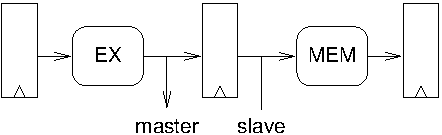
\includegraphics[scale=.8]{fig/ocppipe}
  \caption{Localization of OCP signals in the pipeline}
  \label{fig:ocppipe}
\end{figure}

Figure~\ref{fig:ocppipe} shows the OCP signals in the Patmos
pipeline. The master signals are generated in the execute stage, and
the slave signals are captured in the memory stage.\footnote{For
clarity, the handling of both parts is implemented in the file
\code{Memory.scala}.}
The different variants of the OCP protocol (\code{OCPcore}, \code{OCPcache},
\code{OCPio}, and \code{OCPburst}) in the scope of the Patmos
processor are shown in Figure~\ref{fig:ocplevels}.  

\begin{figure}
  \centering
  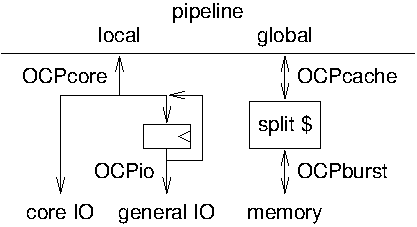
\includegraphics[scale=.8]{fig/ocplevels}
  \caption{OCP levels in Patmos}
  \label{fig:ocplevels}
\end{figure}

\subsection{OCPcore}

This is the simplest variant of the OCP protocol used in Patmos
and shall be used for IO devices.
The variant of OCP is generated by the pipeline for the local address
space. 
\code{OCPcore} is tailored to accesses to
on-chip memories, which on FPGAs necessarily include an
registers on the input ports (read and write address, write data, and write enable).
Furthermore, \code{OCPcore} is the interface for general IO devices. 
The respective signals are shown in
Table~\ref{tab:coresignals}.
To enable sub-word transfers of data, the signal
\code{MByteEn} is used.

\code{OCPcore} is a simple protocol with single cycle command
and reply. A read (\code{RD}) or write (\code{WR}) command is valid
for a single cycle. A data response for a read includes the reponse
\code{DVA} and is expect earliest in the following cycle.
Writes also need to be acknowledged with a \code{DVA} response
(earliest in the following cycle).
The slave can delay the response for arbitrary cycles.
The following assumptions apply:
\begin{itemize}
\item Only reads (\code{RD}) and writes (\code{WR}) are
  supported. Writes require a response (\code{writeresp\_enable=1}),
  such that every command must be followed by a response.
\item No \code{SCmdAccept} or \code{MRespAccept}, flow control is done
  solely via \code{SResp}.
\item Slaves may generate responses earliest in the cycle after a
  command.
\item The master may issue commands in the same cycle as the slave
  sends its response, i.e., basic support for pipelining is required.
\item \code{MByteEn} is assumed to be properly aligned
  (\code{force\_aligned=1}). The signal can be ignored for read
  accesses without side effects.
\end{itemize}

\begin{table}
  \centering
  \caption{\code{OCPcore} signals}
  \label{tab:coresignals}
  \begin{tabular}{ll}
    \toprule
    Signal & Description \\
    \midrule
    \code{MCmd} & Command (\code{RD} or \code{WR}) \\
    \code{MAddr} & Address, byte-based, lowest two bits always 0 \\
    \code{MData} & Data for writes, 32 bits \\
    \code{MByteEn} & Byte enables for sub-word accesses, 4 bits \\
    \cmidrule{1-2}
    \code{SResp} & Response (\code{NULL} or \code{DVA}) \\
    \code{SData} & Data for reads, 32 bits \\
    \bottomrule
  \end{tabular}
\end{table}

Figure~\ref{fig:timing_core} shows a sequence read/write/read in
\code{OCPcore}, where the slave responds to the first read in the following
cycle (the earliest possibility). The write response is delayed by one cycle.
The second read response is also delayed by an additional cycle.

\begin{figure}
\centering
\includegraphics{fig/timing_core}
\caption{Timing diagram for \code{OCPcore}}
\label{fig:timing_core}
\end{figure}

\begin{enumerate}[A:]
\item The master issues a read by setting \code{MCmd} to \code{RD},
  \code{MAddr} to \code{A$_1$} and \code{MByteEn} to \code{E$_1$}.
\item The slave responds to the read issued in cycle A by setting
  \code{SResp} to \code{DVA} and returning the appropriate data. The
  master can issue the next command in the same cycle as it receives
  the response and issues a write command \code{WR}. The
  master provides the byte enable value \code{E$_2$} along with the
  data \code{D$_2$} to specify which bytes should be actually written.
\item The slave does not respond immediately and the master is
  stalled. \code{MCmd} must be \code{IDLE} while the master is
  stalled.
\item The slave responds to the write issued in cycle B. The master
  issues a read in the same cycle.
\item The slave does not respond to the read request, delaying it by one cycle.
\item The slave responds to the read request issued in cycle D.
\item The interface is idle.
\end{enumerate}

\subsection{OCPcache}

This OCP variant is generated for the global address space and is used
for communication between the pipeline and the caches. It is the same
as \code{OCPcore}, but includes an additional signal \code{MAddrSpace}
to specify the cache that should serve the access.

\subsection{OCPio}

The \code{OCPio} level is derived from the \code{OCPcore} level by
inserting a register in the master signals. \code{OCPio} contains
additional signals and all signals are shown in Table~\ref{tab:ocpiosignals}.
This interface is needed to support clock domain crossing.
Currently it is only used at the interface to the configuration port
of the Argo network-on-chip.

\code{OCPio} is slightly more
flexible than \code{OCPcore} and appropriate for I/O devices that do
not (or cannot) follow the semantics of \code{OCPcore}. Registering
the master signals changes the protocol as follows:
\begin{itemize}
\item Slaves may generate responses in the same cycle as they
  receive a command.
\item Commands are issued earliest in the cycle after a response (no
  pipelining).
\item \code{SCmdAccept} is supported. It is sufficient to register the
  master signals only if the currently registered command is
  \code{IDLE} or \code{SCmdAccept} is high.
\item In order to have symmetric handshaking for commands and
  responses and to facilitate clock-domain crossing, \code{OCPio} also
  includes a signal \code{MRespAccept}. An \code{OCPio} port that is
  derived directly from the pipeline's \code{OCPcore} port always
  accepts responses.
\end{itemize}

\begin{table}
  \centering
  \caption{\code{OCPio} signals}
  \label{tab:ocpiosignals}
  \begin{tabular}{ll}
    \toprule
    Signal & Description \\
    \midrule
    \code{MCmd} & Command \\
    \code{MAddr} & Address, byte-based, lowest two bits always 0 \\
    \code{MData} & Data for writes, 32 bits \\
    \code{MByteEn} & Byte enables for sub-word accesses, 4 bits \\
    \code{MRespAccept} & Enable handshaking with \code{SResp} \\
    \cmidrule{1-2}
    \code{SResp} & Response \\
    \code{SData} & Data for reads, 32 bits \\
    \code{SCmdAccept} & Flow control towards the command from the master \\
    \bottomrule
  \end{tabular}
\end{table}

Figure~\ref{fig:timing_io} shows a sequence read/write/read in
\code{OCPio}, where the slave does not accept the write immediately
and delays the response to the write by one cycle.

\begin{figure}
\centering
\includegraphics{fig/timing_io}
\caption{Timing diagram for \code{OCPio}}
\label{fig:timing_io}
\end{figure}

\begin{enumerate}[A:]
\item The master issues a read by setting \code{MCmd} to
  \code{RD}. The slave accepts the command by setting
  \code{SCmdAccept} to high and responds immediately by setting
  \code{SResp} to \code{DVA} and returning the appropriate data.
\item The master issues a write command \code{WR} with
  data \code{D$_2$} and byte enables \code{E$_2$}. The slave
  signals that it does not accept the command by setting
  \code{SCmdAccept} to low.
\item As the slave did not accept the command in cycle B, the master
  still issues the command. The slave accepts the command by setting
  \code{SCmdAccept} to high.
\item The slave responds to the write it accepted in cycle C. Note
  that a) the master is not allowed to issue a new command immediately
  and b) \code{SCmdAccept} may take any value, because \code{MCmd} is
  \code{IDLE}.
\item The master issues a read to which the slave responds immediately.
\end{enumerate}

\subsection{OCPburst}

The caches access the external memory through bursts only;
Table~\ref{tab:burstsignals} shows the signals of the \code{OCPburst}
interface. The tie-off value for \code{MBurstLength} is 4, and
\code{MBurstSingleReq} is tied off to 1. This means that the master
supplies four data words for each write command, and the slave returns
four words for each read command. The burst length is configurable,
but might be restricted by the external memory and the external
memory controller.
\martin{I assume (hope) that the configurable burst length works.
One could try varying with the SRAM memory.} 
\wolf{Depends on how cleanly the code was written and on the
  hardware. The synchronous SRAM only supports burst lengths $\leq$4
  due to restrictions of the memory chip.}
All other burst-related signals are
tied off to their default values. This entails that the only sequence
for burst addresses is \code{INCR}. Bursts always start at an address
that is aligned to the burst size
(\code{burst\_aligned=1}). Furthermore, \code{reqdata\_together} is
set to 1, i.e., write commands and the respective first word are
issued together. Instead of the signal \code{MByteEn}, \code{OCPburst}
uses the signal \code{MDataByteEn}. This implies that partial write
transfers are fully supported, but partial read commands are
unsupported.

We assume that the master provides data for burst accesses in
consecutive cycles and that slaves can accept all burst data words
once they accept the first word. To enable handshaking for the
acceptance of the first data word, the \code{OCPburst} variant
includes the signals \code{MDataValid} and \code{SDataAccept}. As
\code{reqdata\_together} is set to 1, delaying the acceptance of data
also delays the acceptance of write commands. In order to do the same
for read commands, \code{OCPburst} also includes the signal
\code{SCmdAccept}. The signals \code{SCmdAccept} and
\code{SDataAccept} can be generated by the same logic. For the
acceptance of write commands they must be identical, otherwise at
least one of the signals can have an undefined value. We assume that
slaves return burst read data in consecutive cycles.

The first response to a read command may be given in the cycle after
the command. The response to a write command may be given earliest in
the cycle after the last data word was sent. Commands may be issued
earliest in the cycle after the last response from an earlier command
is received.
\martin{Having a write response one cycle after the last data and not
allowing a command in that cycle costs us one additional clock cycle
(in the TDM slot). Maybe it doe not matter.}
\wolf{The consensus was that it would not matter. We could change it
  if we make sure all slaves comply, the restriction was basically just
  put in to be on the safe side.}

\begin{table}
  \centering
  \caption{\code{OCPburst} signals}
  \label{tab:burstsignals}
  \begin{tabular}{ll}
    \toprule
    Signal & Description \\
    \midrule
    \code{MCmd} & Command \\
    \code{MAddr} & Address, byte-based, lowest two bits always 0 \\
    \code{MData} & Data for writes, 32 bits \\
    \code{MDataByteEn} & Byte enables for sub-word writes, 4 bits \\
    \code{MDataValid} & Signal that data is valid, 1 bit \\
    \cmidrule{1-2}
    \code{SResp} & Response \\
    \code{SData} & Data for reads, 32 bits \\
    \code{SCmdAccept} & Signal that command is accepted, 1 bit \\
    \code{SDataAccept} & Signal that data is accepted, 1 bit \\
    \bottomrule
  \end{tabular}
\end{table}

Figure~\ref{fig:timing_burst} shows a read followed by a write in
\code{OCPburst}, were the slave does not accept the first data word
immediately.

\begin{figure}
\centering
\includegraphics{fig/timing_burst}
\caption{Timing diagram for \code{OCPburst}}
\label{fig:timing_burst}
\end{figure}

\begin{enumerate}[A:]
\item The master issues a read command by setting \code{MCmd} to
  \code{RD}. The slave accepts by asserting \code{SCmdAccept}.
\item The slave provides the first response \code{DVA$_{1.0}$}, with
  data from address \code{A$_1$}.
\item The slave provides the second response \code{DVA$_{1.1}$}, with
  data from address \code{A$_1$+4}.
\item The slave provides the third response \code{DVA$_{1.2}$}, with
  data from address \code{A$_1$+8}.
\item The slave provides the fourth and last response
  \code{DVA$_{1.3}$}, with data from address \code{A$_1$+12}.
\item The master issues a write command by setting \code{MCmd} to
  \code{WR} and provides the first data word \code{D$_{2.0}$} width
  byte enables \code{E$_{2.0}$} It signals that the data is valid by
  asserting \code{MDataValid}. The slave signals that it cannot accept
  the data by setting \code{SDataAccept} to low.
\item As the slave did not accept the data in cycle F, the master
  keeps issuing the command and providing the data word
  \code{D$_{2.0}$}. The slave now accepts the data by setting
  \code{SDataAccept} to high.
\item The master provides the second data word, \code{D$_{2.1}$} with
  byte enables \code{E$_{2.1}$}.
\item The master provides the third data word, \code{D$_{2.2}$} with
  byte enables \code{E$_{2.2}$}.
\item The master provides the fourth and last data word,
  \code{D$_{2.3}$} with byte enables \code{E$_{2.3}$}.
\item The slave responds to the write burst by setting \code{SResp} to
  \code{DVA}.
\end{enumerate}

\subsection{Remarks}

\code{SCmdAccept} is valid only while a command is unequal to
\code{IDLE}. Consequently, \code{SCmdAccept} must be properly
multiplexed to support multiple slaves. For handshaking via
\code{SResp}, it is sufficient to combine the responses of different
slaves with OR.

In \code{OCPcore} and \code{OCPcache}, slaves accept commands
implicitly. Asserting a command for more than one cycle corresponds to
issuing two separate commands. This is only allowed if the slave
responds in the cycle immediately after the first command. In
\code{OCPio} and \code{OCPburst}, slaves accept commands in the cycle
where they assert \code{SCmdAccept}. Continuing to assert a command in
the next cycle corresponds to a separate command. This is disallowed
in \code{OCPburst}, and allowed in \code{OCPio} only if the slave
responds immediately in the cycle where it asserts \code{SCmdAccept}.

\wolf{\code{OCPburst} currently allows neither pipelining nor
  same-cycle responses. If we want to, we can make it more like
  \code{OCPcore} or \code{OCPio}.}

The burst length is restricted to a constant which is a power of 2.
The address must be aligned. Burst data must be provided in
consecutive cycles. For reads, \code{SResp} is active during these
cycles and the number of responses must always match the burst length.
Error responses (where SResp has value \code{ERR}) may not abort the
response sequence prematurely. For a burst write, the master may have
to provide D1 for two or more cycles if \code{SDataAccept} is not
active in the first cycle of the transaction.

As the first data word must be accepted together with the command and
we require burst data to be provided in consecutive cycles, the
signals \code{MDataValid} and \code{SDataAccept} may appear to be
superfluous. However, they are required by the OCP standard for the
inclusion of the \code{MDataByteEn} signal, which provides separate
byte enables for each word in a burst transaction.

\martin{Burst: Is it legal (in our OCP subset) that SCmdAccept comes earlier than SDataAccept?} \wolf{No. Masters can assume that both signals are asserted in the same cycle.}

\martin{Burst: we said that we do not support pipelined requests in burst mode.
So when the slave sets SResp we are not allowing the master to initiate the next
request in the same cycle. Right?} \wolf{Right.}

\section{Example I/O Device}
\label{sec:exampleio}

In this section we summarize the chapter by showing how to build a simple
I/O device, a counter.
Several examples of I/O devices can be found in \code{patmos/hardware/src/io}.
Adding an I/O device to Patmos consists of 2--3 steps:

\begin{itemize}
\item Describing the I/O device in Chisel
\item Adding the device and the address into the configuration file
\item If the device contains pins to the external world, the pins need to be added to
the top-level (VHDL) file and to the Quartus (.qsf) or Xilinx configuration files
\end{itemize}


An I/O device has to extend \code{CoreDevice} and needs to define a
companion object that extends \code{DeviceObject}. The interface to the
processor is usually \code{OCPcore} where handshaking for the data
is available via \code{SResp}.
In this example we will define a read only device that implements a simple
counter. The complete code for this device can be found in
\code{patmos/hardware/src/io/Counter.scala}.

\begin{lstlisting}[float, caption={Companion object for the counter device\label{lst:ioex:obj}}]
object Counter extends DeviceObject {

  def init(params: Map[String, String]) = {}

  def create(params: Map[String, String]): Counter = Module(new Counter())

  trait Pins {}
}
\end{lstlisting}

Each device needs to define a companion object that is used as a factory
object to create devices and needs to overwrite two methods: \code{init()}
and \code{create()} and needs to overwrite the trait \code{Pins}.
Listing~\ref{lst:ioex:obj} shows the the companion object for our counter
device. The method \code{init()} can be used to pass parameters from the
configuration file (e.g., altde2-115.xml). As we do not use parameters in our
simple example we just define an empty method. The method \code{create()}
is the singleton method that shall return an instance of an I/O device.
In our example we create one \code{Counter} object, wrap it into a \code{Module},
as any Chisel component, and return it from \code{create()}. The method
\code{create()} itself can receive parameters, which we do not use in this example.

\begin{lstlisting}[float, caption={Class for the counter device\label{lst:ioex:class}}]
class Counter() extends CoreDevice() {

  io.ocp.S.Data := UInt(42)
  
  val respReg = Reg(init = OcpResp.NULL)
  
  respReg := OcpResp.NULL
  when(io.ocp.M.Cmd === OcpCmd.RD) {
    respReg := OcpResp.DVA
  }
  
  io.ocp.S.Resp := respReg
}
\end{lstlisting}

Listing~\ref{lst:ioex:class} shows the first, incomplete, version of our I/O device.
We simply return 42 on a read from the device. However, we also need to
adhere to the OCP signaling. We need to response to a read command
in the next clock cycle with a data valid signal (\code{DVA}). Otherwise we need to
set the response to \code{NULL}.

Note that the read needs to be valid in the very same cycle when
the output of \code{respReg} becomes \code{DVA}.
In the first version of this example we ignore writes to the counter.\footnote{If we write
to the counter device, the device will not generate a \code{DVA}
for \code{Resp} and therefore stall the pipeline forever.
A complete design should at least ignore writes, but response to them.}

\begin{lstlisting}[float, caption={Configuring the processor to include our
counter device\label{lst:ioex:xml}}]
<IO DevTypeRef="Counter" offset="11"/>

<Dev DevType="Counter" entity="Counter" iface="OcpCore"/>
\end{lstlisting}

Listing~\ref{lst:ioex:xml} shows the last step, configuring Patmos to use the
counter. In our example we change the configuration file that is used for
the default configuration: \code{patmos/hardware/config/altde2-115.xml}.
The two lines from Listing~\ref{lst:ioex:xml} need to added into section \code{IOs}
and \code{Devs}, respectively. Offset 11 is the next available I/O address and
results in mapping our counter to I/O address \code{0xf00b0000}
(each I/O device has a 16 bit local address and 11 in decimal is `b' in hexadecimal).

\begin{lstlisting}[float, caption={Testing the counter device\label{lst:ioex:c}}]
#include <machine/patmos.h>
#include <stdio.h>

int main() {

  volatile _IODEV int *io_ptr = (volatile _IODEV int *) 0xf00b0000;
  int val;

  val = *io_ptr;
  printf("%d\n", val);
}

\end{lstlisting}

Listing~\ref{lst:ioex:c} shows a small test program to read our counter device
and write the value to stdout. As our I/O device lives in the local memory
area we need to tell the C compiler to the local load and store instructions
to access the I/O device. This is performed by defining a special pointer
with the macro \code{\_IODEV}, which we import by including \code{<machine/patmos.h>}.

\begin{lstlisting}[float, caption={Chisel code for counting\label{lst:ioex:cnt}}]
  val countReg = Reg(init = UInt(0, 32))
  countReg := countReg + UInt(1)
  io.ocp.S.Data := countReg
\end{lstlisting}

To implement a counter we need a register and some addition.
Listing~\ref{lst:ioex:cnt} hows the Chisel code for this free running counter.
We now have a device the ticks at the processor frequency and can be used
to measure execution time. Listing~\ref{lst:ioex:measure} shows how to use
our counter to measure the execution time of the \code{printf} function with a simple
string print out.

\begin{lstlisting}[float, caption={Measure execution time\label{lst:ioex:measure}}]
  val1 = *io_ptr;
  printf("Hello");
  val2 = *io_ptr;

  printf("Execution time is %d\n", val2-val1);
\end{lstlisting}

\begin{lstlisting}[float, caption={A writable counter\label{lst:ioex:write}}]
class Counter() extends CoreDevice() {

  val countReg = Reg(init = UInt(0, 32))
  countReg := countReg + UInt(1)
  when (io.ocp.M.Cmd === OcpCmd.WR) {
    countReg := io.ocp.M.Data 
  }
  
  val respReg = Reg(init = OcpResp.NULL)
  respReg := OcpResp.NULL
  when(io.ocp.M.Cmd === OcpCmd.RD || io.ocp.M.Cmd === OcpCmd.WR) {
    respReg := OcpResp.DVA
  }
  
  io.ocp.S.Data := countReg  
  io.ocp.S.Resp := respReg
}
\end{lstlisting}

To complete the example we add a write to the device where we can set
the value of the counter. Listing~\ref{lst:ioex:write} shows the complete
code of our counter where we can set the value. On a OCP write we take the
data value in the same clock cycle as input to the counter register.
As with the read operation, we acknowledge the write in the following clock
cycle with a \code{DVA}.

When the I/O device has more than one register (or some memory), the
address signals from the OCP connection (\code{io.ocp.M.Addr}) are used
for address decoding. See for an example the \code{CpuInfo} device.




% % % % % % % % % % % % % % % % % % % % % % % % % % % % % % % % % % % % % % % %
\chapter{Application Binary Interface}
\label{sec:abi}

\section{Data Representation}

Data words in memories are stored using the big-endian data representation, this
also includes the instruction representation.

\section{Register Usage Conventions}

The register usage conventions for the general purpose registers are as follows:
\begin{itemize}
  \item \texttt{r0} is defined to be zero at all times.
  \item \texttt{r1} and \texttt{r2} are used to pass the return value on
        function calls. \\
        For 64 bit results, the high part is stored in \texttt{r1},
        the low part in \texttt{r2}.
	32 bit results are returned using \texttt{r1} only.
  \item \texttt{r3} through \texttt{r8} are used to pass arguments on function
        calls. \\
        For 64 bit arguments, the high part is stored first,
        followed by the low part.\\ E.g., for a 64 bit argument passed in
        \texttt{[r3,r4]}, the high part is in \texttt{r3}, the low part
        in \texttt{r4}.
  \item \texttt{r29} is used as temp register.
  \item \texttt{r30} is defined as the frame pointer and
        \texttt{r31} is defined as the stack pointer for the \emph{shadow}
        stack in global memory.
        The use of a frame pointer is optional, the register can freely be
        used otherwise.
	\texttt{r31} is guaranteed to always hold the current stack pointer and
        is not used otherwise by the compiler.
  \item \texttt{r1} through \texttt{r19} are caller-saved \emph{scratch}
        registers.
  \item \texttt{r20} through \texttt{r31} are callee-saved \emph{saved}
        registers.
\end{itemize}

The usage conventions of the predicate registers are as follows:
\begin{itemize}
  \item all predicate registers are callee-saved \emph{saved} registers.
\end{itemize}


\stefan{We would gain in most cases by making predicates caller-saved, since predicates are usually not
used across function calls, this saves up to 6 instructions per call.
Predicate live ranges over calls only happen with single-path and if-conversion. However, having only caller-saved predicates
makes if-conversion of calls too costly (and too complex). A nicer solution would be to have p1-p4 caller-saved and
p5-p7 callee saved. I got this to work (do not alias s0 with p1-p7 in RegInfo.td, mark s0 and p5-p7 as callee saved
in RegInfo.cpp, and in processBeforeCalleeSavedScan set s0 as used when any of p5-p7 is used), but this would require the
if-converter to use callee-saved predicates when converting calls, i.e., to change the predicate of the condition.
Sounds easy, but is actually far from trivial to hack into the if-converter, and only works if the if-converter runs before the
prologue-inserter, so we stay with callee saved registers for now and live with the costs of spilling s0 at nearly every call.}
\daniel{It would also break the single-path conversion pass.}

The usage conventions of the special registers are as follows:
\begin{itemize}
  \item \texttt{s0}, representing the predicate registers, is a callee-saved
        \emph{saved} register.
  \item The stack cache control registers \texttt{ss} and \texttt{st} are
        callee-saved \emph{saved} registers.
  \item The return information registers \texttt{s7-s10} (\texttt{srb},
        \texttt{sro}, \texttt{sxb}, \texttt{sxo}) are callee-saved
        \emph{saved} registers.
  \item All other special registers are caller-saved scratch registers and
        should not be used across function calls.
\end{itemize}



\section{Function Calls}
\label{sec:function_calls}

Function calls have to be executed using the \texttt{call}
instruction that automatically prefetches the target function to the method
cache and stores the return information in the special registers \texttt{srb}
and \texttt{sro}.

The register usage conventions of the previous section indicate which registers
are preserved across function calls.

The first $6$ arguments of integral data type are passed in registers, where
64-bit integer and floating point types occupy two registers. All other
arguments are passed on the \emph{shadow} stack via the global memory.

\fb{We could pass arguments via the stack cache, however, this would work only
for functions with a fixed number of arguments. The calling convention for
variadic function would then differ from the standard conventions. We should
probably also introduce a size limit on how many arguments should be passed via
the stack cache. Thus, for a first shot I decided to keep the conventions
simple.}
\martin{I would like to see arguments passed via the stack cache. No
reason to go via main memory (when the number is fixed.}

\martin{BTW: an on-chip stack, with single cycle access, is not so different from
a large register file. Maybe using a sliding window to keep the number of
addressing bits down. Shall we merge the stack cache with the register file?
Are we than redoing a stack (Java) processor?}

When the return function base \texttt{srb} and the return offset \texttt{sro}
needs to be saved to the stack, they have to be saved as the first elements of
the function's stack frame, i.e., right after the stack frame of the calling
function.
%
Note that in contrast to \texttt{br} and \texttt{brcf} the return offset refers
to the next instruction after the \emph{delay slot} of the corresponding
\texttt{call} and can be implementation dependent (cf.\ the description of the
\texttt{call} and \texttt{ret} instructions).

\section{Sub-Functions}
A function can be split into several sub-functions. The program is only allowed to use
\texttt{br} to jump within the same sub-function. To enter a different sub-function,
\texttt{brcf} must be used. It can only be used to jump to the first instruction of a
sub-function.

In contrast to \texttt{call}, \texttt{brcf} does not provide link information.
Executing \texttt{ret} in a sub-function will therefore return to the last \texttt{call}, not to the last \texttt{brcf}.
Function offsets however are relative to the \emph{sub-function} base, not to the surrounding function.
The function base register \texttt{r30} must therefore be set to the base address
of the current \emph{sub-function} for calls inside sub-functions.

A sub-function must be aligned and must be prefixed with a word containing the size of the sub-function,
like for a regular function. If a function is split into sub-functions, the first sub-function
must also be prefixed with the size of the first sub-function, not with the size of the whole function.

There are no calling conventions for jumps between sub-functions, for the compiler
this behaves just like a regular jump.
% except that the base register texttt{srb} must be updated if the
% sub-function contains calls.


% TODO: examples

\stefan{We need to define how the call and local branch with cache fill get the size of the code to load. A word
containing the size at the target address, or prior to the target address? (including or excluding the size word?)}

\jack{I'd store the code size at the target address and have the
method itself start at an offset +4 or +8 from that place. I also
suggest storing the stack size here too. Could fit into the same
32-bit word (since I'd guess the local memory size limits us to
$<64$k code and $<64$k stack in a single method anyway).}

\martin{Agree for plain C code where there is no data structure
further describing a function. In the JOP JVM I have the luxury
to have those sizes as part of the virtual method dispatch table.
One indirection is there needed anyway, so why not having those
data there.}

\section{Stack Layout}

All stack data in the global memory, either managed by the stack cache or using
a frame/stack pointer, grows from top-to-bottom. The use of a frame pointer is
optional.

Unwinding of the call stack is done on the stack-cache managed stack frame,
following the conventions declared in the previous subsection on function calls.

\section{Interrupts and Context Switching}

\daniel{TODO update}

Interrupt handlers may use the shadow stack pointer \texttt{r29} to spill registers
to the shadow stack. Interrupt handlers must ensure that all special registers
that might be in use when the interrupt occurs % MS: there is probably no 'might' WP: not all special registers are used, e.g., s11-s15
are saved and restored.
%
Here is an example of storing and restoring the context for context switching.
\begin{verbatim}
sub $r29 = $r29, 40
sws [$r29 + 0] = $r31
sws [$r29 + 1] = $r30
sws [$r29 + 2] = $r22  // free some registers
sws [$r29 + 3] = $r23
mfs $r22 = $s2  // by now any mul should be finished
mfs $r23 = $s3
sws [$r29 + 4] = $r22
sws [$r29 + 5] = $r23
mfs $r22 = $s5  // read out cache pointers, spill
mfs $r23 = $s6
sub $r22 = $r23, $r22
sspill $r22   // spill the memory, s5 == s6 now
sws [$r29 + 6] = $r22  // store the stack pointer
sws [$r29 + 7] = $r23  // store stack size
...
// TODO store return base and offset

// restore
lws $r23 = [$r29 + 7]
lws $r22 = [$r29 + 6]
mts $s5 = $r22   // restore the stack
mts $s6 = $r22
sens $r23
lws $r23 = [$r29 + 5]
lws $r22 = [$r29 + 4]
mts $s2 = $r22
mts $s3 = $r23
....
\end{verbatim}




% % % % % % % % % % % % % % % % % % % % % % % % % % % % % % % % % % % % % % % %
\chapter{Implementation}

\martin{This sections shall describe implementation details,
decisions, and options.}

After a first implementation of Patmos in VHDL we did a cleanup and
rewrite in a the hardware description language Chisel~\cite{chisel:dac2012}.
The following notes on the implementation of Patmos and implementation
decisions is based on first design discussions within the VHDL version
and concrete implementation experiments with Chisel. All size and frequency
numbers are from the Chisel implementation. A comparison between VHDL
and Chisel would be of great interest.

For a comparison between Chisel and VHDL we take a snapshot when both
versions where about at the same functionality: LoC, excluding the copyright
header at 6.4.2013: Chisel: 996 VHDL: 3020. However, the VHDL code was
written quite verbatim and more usage of \code{record} would probably result
in about 2000 L0C. Still Chisel is more compact and probably easier readable.


\section{Component Organization and Pipeline Structure}

The architecture of Patmos is structured around five components, each
representing one pipeline stage. Each component contains the \emph{left}
pipeline register. E.g., the output of the \code{DEC} stage (decode signals,
the two register values, and the immediate field) is combinatorial from
the decode stage and registered in the \code{EX} stage. The motivation of
this organization is that input registers of on-chip memory elements (e.g., instruction
memory, register file, and data memory) are part of the pipeline register.
They need to be fed unconditionally from the unregistered output of
the former stage.

Each stage has exactly one pipeline register, which is placed at the begin
of the component. The pipeline registers use an enable for stalling.
Register that have no enable (input registers of on-chip memories) need
a \emph{shadow} register and a multiplexer for stalls.

The interface from the EX stage to the MEM stage might use one
field for ALU results and the store data or individual fields. Individual
fields might reduce the pressure on the ALU multiplexers.
\martin{Update to the current implementation -- check for difference.}


\section{Register File}

There are two options to implement the register file (RF) in an FPGA: (1) use
two on-chip memories to provide two read ports and one write port, or (2)
use dedicated registers and larger multiplexer structures for the read
ports. Usually one aims to use on-chip memory for the RF. However,
in a design constraint largely by the available amount of on-chip memory,
a RF built out of registers might be preferable.

For a dual issue pipeline we need 4 read ports and 2 write ports into the RF.
We explored double clocking of a on-chip based RF in~\cite{patmos:ppes2011}.
It is feasible, the resulting maximum frequency fits for the ALU path, but feels
a little bit brittle. A RF from registers might give a more robust design for the
two write ports.

The ideal solution would be to make it configurable if on-chip memory or
LCs are used. The issue width should also be configurable.




\section{Resource and Fmax Numbers}

State 13.3.2013 with Chisel and DE2-70: A shared field (for EX to MEM?) results 3435 LCs
and 81.7 MHz, two fields in 3499 LCs and 81.8 MHz. Looks like not a big deal,
but just 64 more LCs. Where does this cost come from? A very inefficient
enable on the pipeline register (MUX instead of an enable signal?).

\martin{Update with reduced ALU muxes and also with additional second
ALU pipeline (forwarding). Is dual issue configurable?}

\section{ALU Discussion}

The large multiplexers and the forwarding limit the maximum frequency.
We have already removed the expensive rotate instructions and the
\code{abs} instruction.

Current version (4.4.2013) with all ALU operations and test case ALU.s
for the DE2-70 is: 3415 LCs, 85.44 MHz. Dropping \code{rsub} and all unary
ALU operations: 3173 LCs, 91.91 MHz.

\todo{This should be updated. Maybe even with some statistics how the size
(and performance ?) changed over time.}


%%%%%%%%%%%%%%%%%%%%%%%%%%%%%%%%%%%%%%%%%%%%%%%%%%%%%%%%%%%%%%%%%%%%%%%%%%%%%%
\chapter{Build Instructions}
\label{ch:build_instructions}

In the following we describe: (1) the installation of needed tool under Ubuntu and
on Mac OS X, (2) how to build the Patmos tool chain (e.g., compiler), and (3) how
to get started with Patmos.

The installation instructions might also be valid on different Linux versions.
Patmos and the compiler have also been successfully installed on a Mac OS X
system.  The support of Windows is marginal, or basically not existent.

For an easier start we provide a VM image with Ubuntu 14.04 including
all tools installed for download from: \url{http://patmos.compute.dtu.dk/}


% ------------------------------------------------------------------------------
%\section{Prerequisites}
%
%In order to build all tools, the following programs and libraries are required:
%
%\begin{itemize}
%\item[cmake, make] \hfill\\
%The CMake (at least version 2.8) and \texttt{make} build systems are required to build the
%various components of the tool chain, such as the \texttt{clang} compiler or the \texttt{compiler-rt} system library.
%\medskip
%
%\item[gcc, g++] \hfill\\
%A C and C++ compiler such as GCC is required to build \texttt{clang}, \texttt{llvm}
%and \texttt{gold}. It is also possible to use a separate \texttt{clang} installation as
%an alternative to GCC. Compiling with \texttt{clang} will result in shorter compile
%times, but at least version 3.3 is required.
%\medskip
%
%\item[flex, bison, texinfo] \hfill\\
%These tools are required to build tools such as gold successfully.
%\medskip
%
%\item[libelf] \hfill\\
%The tools in the Patmos tool chain require the development headers of \texttt{libelf},
%as this library is used to read and write ELF files.
%\medskip
%
%\item[boost] \hfill\\
%The simulator requires the program-options library from the \texttt{boost} C++ library
%(at least version 1.46).
%\medskip
%
%\item[git, subversion] \hfill\\
%The version control system \texttt{git} and \texttt{svn} are required
%to download the latest development versions of the tools and the benchmarks.
%\end{itemize}
%

\section{Setup on Ubuntu and Mac OS X}

In the following we present the Patmos build instructions including setup of
tools in Ubuntu and for the Mac OS X.

\subsection{Setup on Ubuntu 16.04 LTS 64-Bit}

In the following we present the setup of tools within a recent Ubuntu version.
Here is the list of needed (or recommended) packages:

\begin{verbatim}
sudo apt-get install git default-jdk gitk cmake make g++ texinfo flex bison \
  subversion libelf-dev graphviz libboost-dev libboost-program-options-dev ruby-full \
  liblpsolve55-dev python zlib1g-dev gtkwave gtkterm scala
\end{verbatim}

Install \code{sbt} with:

\begin{verbatim}
echo "deb https://dl.bintray.com/sbt/debian /" | sudo tee -a /etc/apt/sources.list.d/sbt.list
sudo apt-key adv --keyserver hkp://keyserver.ubuntu.com:80 \
  --recv 2EE0EA64E40A89B84B2DF73499E82A75642AC823
sudo apt-get update
sudo apt-get install sbt
\end{verbatim}

For the Quartus setup it is best to change the default shell to \code{/bin/bash}:

\begin{verbatim}
sudo rm /bin/sh
sudo ln -s /bin/bash /bin/sh
\end{verbatim}


For building the Patmos documentation (e.g., the handbook) you need to install
a full version of LaTeX (about 3~GB) with:

\begin{verbatim}
sudo apt-get install texlive-full doxygen
\end{verbatim}

%\subsection{Setup On Ubuntu 14.04 LTS 32-Bit}
%
%In the following we present the Patmos build instructions on a 32-bit Linux/Ubuntu
%system (14.04 LTS).\footnote{I used the 32-bit version of Ubuntu to simplify the Quartus installation.}
%
%After a plain Ubuntu installation several packages need to be installed.
%The following apt-get lists the packages that need to be
%installed:\footnote{Some packages might be available in newer version
%when reading this document.}
%
%\begin{verbatim}
%sudo apt-get install git openjdk-7-jdk gitk cmake make g++ texinfo flex bison \
%  subversion libelf-dev graphviz libboost-dev libboost-program-options-dev ruby1.9.1 \
%  ruby1.9.1-dev liblpsolve55-dev python zlib1g-dev gtkwave gtkterm scala
%\end{verbatim}
%
%\emph{The following gem install might not be needed as with the correct
%packages (liblpsolve55-dev) the setup script shall do it automatically.
%Needs to be checked on a fresh Ubuntu machine.
%This is done after T-CREST has been installed.}
%
%From within \code{llvm/tools/platin} install:
%
%\begin{verbatim}
%sudo gem1.9.1 install lpsolve --pre
%sudo gem1.9.1 install ext/lpsolve-5.5.10.j.gem
%\end{verbatim}
%
%Install \code{sbt} with:
%
%\begin{verbatim}
%wget http://dl.bintray.com/sbt/debian/sbt-0.13.2.deb
%sudo dpkg -i sbt-0.13.2.deb
%sudo apt-get update
%sudo apt-get install sbt
%\end{verbatim}
%
%For the Quartus setup it is best to change the default shell to \code{/bin/bash}:
%
%\begin{verbatim}
%sudo rm /bin/sh
%sudo ln -s /bin/bash /bin/sh
%\end{verbatim}

\subsection{Setup On Mac OS X}

This subsection describes the installation of needed tools and libraries
on Mac OS X. It is based on a OS X Yosemite and assumes to use
homebrew\footnote{\url{http://brew.sh/}} for package management.

First install the Mac compiler (Xcode) and the command line tools.

For the build of Patmos and the compiler we need to install:

\begin{verbatim}
brew install cmake boost libelf sbt doxygen
\end{verbatim}

Mac OS X comes with Python version 2.7 preinstalled. For Aegean
we need Python 3 and the xml library that can be installed with:

\begin{verbatim}
brew install python3
pip3 install lxml
\end{verbatim}

For WCET analysis install

\begin{verbatim}
brew install lp_solve
\end{verbatim}

For wave viewing install GTKWave with

\begin{verbatim}
brew install homebrew/x11/gtkwave
\end{verbatim}

\todo{The following should probably be deleted as we switched to homebrew for the setup.}

Several tools are needed, best installed with MacPorts. For Patmos simulator and assembler:
\code{boost}, \code{libelf}.
For simulation with ModelSim: \code{wine}
For Aegean: \code{python33}, \code{py33-lxml}. Make a link from \code{python3} to \code{python3.3} as this is the way it is invoked.
\todo{Alex suggested a way to avoid this by querying how to invoke python.}

\section{Building Patmos and the Compiler Tool Chain}
\label{sec:build:compiler}

We assume that the T-CREST project will live in \code{\$HOME/t-crest}.
Before building Patmos add the path
to the compiler executables (e.g., into your \code{.bashrc} or
\code{.profile}):\footnote{The path needs to be absolute. LLVM cannot handle
a path relative to the home folder \textasciitilde{}, e.g., \code{\textasciitilde{}/t-crest/local/bin}.}

\begin{verbatim}
export PATH=$PATH:$HOME/t-crest/local/bin
\end{verbatim}

A complete logout from Ubuntu might be needed to take effect (just closing
a terminal window is not enough, depending on how you set up your profile files).

Patmos and the compiler can be checked out from GitHub and built as follows:

\begin{verbatim}
mkdir ~/t-crest
cd ~/t-crest
git clone https://github.com/t-crest/patmos-misc.git misc
./misc/build.sh
\end{verbatim}


For developers with push permission generate an ssh key and upload
it at GitHub (see \url{https://help.github.com/articles/connecting-to-github-with-ssh/}
for detailed instructions).
The ssh based clone string for write access is then:

\begin{verbatim}
git clone git@github.com:t-crest/patmos-misc.git misc
./misc/build.sh
\end{verbatim}

This script (\code{build.sh}) will checkout several other repositories (the compiler, library,
and the Patmos source) and
builds the compiler and the Patmos simulator.
Therefore, take a cup of coffee and find some nice reading.

You can test your installation by checking if the compiler is available:

\begin{verbatim}
patmos-clang --version
\end{verbatim}

The \code{build.sh} script contains default options, which should work out of the box. 
The build settings can be changed by a customized \code{misc/build.cfg} file. The file \code{misc/build.cfg.dist}
is an example configuration file containing default values. It is ignored by the build process and should not be
edited.\footnote{It is autogenerated by \code{build.sh -e} from the values in \code{build.sh}.}
To change any options for \code{misc/build.sh}, either start with an empty \code{misc/build.cfg} or
copy \code{misc/build.cfg.dist} and modify the values to your need.


\martin{In Mac OS X I have only .profile and I don't understand what the issue by 'only read by login terminals'.}
\stefan{Login shells are only opened at logins. Interactive terminals are all terminals that are opened by your window manager or
other means. This is why you need to reboot to have .profile take effect. There are slight differences between bash and zsh when which file is read, 
and distribution further mix up the files in non-standard ways.}

\stefan{Relative paths should actually work, but the \textasciitilde{} shortcut is shell-specific and may not work, but
not sure about this.}


For correct signing of your changes set the username and email in git with:

\begin{verbatim}
git config --global user.name "Joe Someone"
git config --global user.email "joe.someone@domain.com"
\end{verbatim}

Optionally, you may additionally add the \code{misc} checkout to your path, so that \code{build.sh} and the helper tools in 
\code{misc} can be executed from everywhere.

\begin{verbatim}
export PATH=$PATH:$HOME/t-crest/misc
\end{verbatim}

The Patmos documentation (handbook, C library, Argo NoC) can be built with:

\begin{verbatim}
cd patmos/doc
make
\end{verbatim}

\section{Quartus on Linux}

Download the free web edition of Quartus from Altera.\footnote{For a 32-bit Linux you need to
use Quartus 13.x as 32-bit support has been dropped from Quartus 14.x.}
The Linux version is
installed as follows:\footnote{\url{http://www.altera.com/literature/manual/quartus_install.pdf}}

\begin{verbatim}
tar xvf Quartus-web-xxx.tar
\end{verbatim}

The software installation is started with:

\begin{verbatim}
bash setup.sh
\end{verbatim}

Then add the \code{bin} directory of Quartus to your \$PATH.
%
For access to the serial port the user needs access rights.

\begin{verbatim}
# Add user to dialout group for the serial port access
sudo usermod -a -G dialout user
\end{verbatim}

Logout and login again to update the group settings.

Getting the Altera USB Blaster working on Ubuntu is a little bit brittle.
Here a collection of tips collected from different places that helped me to
get the USB Blaster running.

The USB devices can be listed with
\begin{verbatim}
lsusb
\end{verbatim}

Add permissions to access the Altera USB Blaster by creating or editing \code{/etc/udev/rules.d/51-usbblaster.rules}:

\begin{verbatim}
# For Altera USB-Blaster permissions.
SUBSYSTEM=="usb",\
ENV{DEVTYPE}=="usb_device",\
ATTR{idVendor}=="09fb",\
ATTR{idProduct}=="6001",\
MODE="0666",\
NAME="bus/usb/$env{BUSNUM}/$env{DEVNUM}",\
RUN+="/bin/chmod 0666 %c"
\end{verbatim}

For the DE10 Nano board following rules are needed:

\begin{verbatim}
SUBSYSTEM=="usb",\
ENV{DEVTYPE}=="usb_device",\
ATTR{idVendor}=="09fb",\
ATTR{idProduct}=="6810",\
MODE="0666",\
NAME="bus/usb/$env{BUSNUM}/$env{DEVNUM}",\
RUN+="/bin/chmod 0666 %c"
\end{verbatim}

Reload the rules:
\begin{verbatim}
sudo udevadm control --reload
\end{verbatim}

Test the JTAG chain with:
\begin{verbatim}
jtagconfig
\end{verbatim}

and hope for an output similar to:

\begin{verbatim}
1) USB-Blaster [2-2.2]
  020F70DD   EP3C120/EP4CE115
\end{verbatim}

In some cases, killing the the jtagd process can make the connection work againg:

\begin{verbatim}
$ sudo killall -9 jtagd
$ sudo killall -9 jtagd # Verify that is not running
jtagd: no process found
$ jtagconfig
\end{verbatim}

Some more fixes might be needed (not on a recent try with Ubuntu 14.04):

\begin{verbatim}
jtagd --foreground --debug
\end{verbatim}

\begin{verbatim}
sudo ln -s /lib/x86_64-linux-gnu/libudev.so.1 /usr/lib/libudev.so.0
jtagconfig -d
\end{verbatim}


After fixing the permissions for the USB Blaster open Quartus and test if the
cable is found with the programmer. Select USB-Blaster in \emph{Hardware Setup}.
When connected to an FPGA test the USB-Blaster with \emph{Auto Detect}
(With the DE2-115, a question about shared JTAG ID pops up -- select EP4CE115).

Quartus~13.1 drops the support of Cyclone~II devices. Therefore, the
(phased out) Altera DE2-70 board is not supported anymore. Version 13.0 supports Cyclone~II\
till Cyclone~V devices and might be the best option at the moment.


\section{The Xilinx ML605 Platform}

For the evaluation within the T-CREST project the Xilinx ML605 FPGA board was chosen as the `standard'
evaluation platform. The T-CREST platform contains, besides several Patmos' connected with the Argo NoC,
a memory tree, called BlueTree, from UoY and the time-predictable memory controller from TU/e. As the
building this platform needs some non-free tools and including closed source code, we provide prebuilt
configurations of the T-CREST platform as bit files available for download:

\begin{itemize}
\item A 4 core version: \url{http://patmos.compute.dtu.dk/t-crest-4core.bit}
\item A 16 core version: 
\end{itemize}

To configure the FPGA use the IMPACT software from Xilinx (command \code{impact}), which is part of the Xilinx ISE package
and needs no license (It is also available in a smaller Lab package). To compile an application and
download it to the ML605 follow the exact same steps as for the Altera CMP version, e.g., from
within the \code{patmos} directory:

\begin{verbatim}
make APP=hello_puts comp download
\end{verbatim}

\subsection{Getting the Xilinx Configuration Cable to Work}

Xilinx does not support Ubuntu (at least the last few versions) directly. The following description
is a summary of the help from Jamie.

Copy some Xilinx cable specific files to \code{/usr/share} with:

\begin{verbatim}
sudo cp /opt/Xilinx/14.7/ISE_DS/ISE/bin/lin/install_script/install_drivers/\
linux_drivers/pcusb/*.hex /usr/share
\end{verbatim}
 
Ensure that \code{fxload} is installed with:
\begin{verbatim} 
sudo apt-get install fxload
\end{verbatim}

Create \code{/etc/udev/rules.d/80-xusbdfw.rules} with following content:

\begin{tiny}
\begin{verbatim}
# version 0003
ATTR{idVendor}=="03fd", ATTR{idProduct}=="0008", MODE="666"
SUBSYSTEM=="usb", ACTION=="add", ATTR{idVendor}=="03fd", ATTR{idProduct}=="0007", RUN+="/sbin/fxload -v -t fx2 -I /usr/share/xusbdfwu.hex -D $tempnode"
SUBSYSTEM=="usb", ACTION=="add", ATTR{idVendor}=="03fd", ATTR{idProduct}=="0009", RUN+="/sbin/fxload -v -t fx2 -I /usr/share/xusb_xup.hex -D $tempnode"
SUBSYSTEM=="usb", ACTION=="add", ATTR{idVendor}=="03fd", ATTR{idProduct}=="000d", RUN+="/sbin/fxload -v -t fx2 -I /usr/share/xusb_emb.hex -D $tempnode"
SUBSYSTEM=="usb", ACTION=="add", ATTR{idVendor}=="03fd", ATTR{idProduct}=="000f", RUN+="/sbin/fxload -v -t fx2 -I /usr/share/xusb_xlp.hex -D $tempnode"
SUBSYSTEM=="usb", ACTION=="add", ATTR{idVendor}=="03fd", ATTR{idProduct}=="0013", RUN+="/sbin/fxload -v -t fx2 -I /usr/share/xusb_xp2.hex -D $tempnode"
SUBSYSTEM=="usb", ACTION=="add", ATTR{idVendor}=="03fd", ATTR{idProduct}=="0015", RUN+="/sbin/fxload -v -t fx2 -I /usr/share/xusb_xse.hex -D $tempnode"
\end{verbatim}
\end{tiny}

Restart the udev service with:

\begin{verbatim} 
sudo udevadm control --reload-rules
\end{verbatim}

Make sure that libusb is installed (e.g., in \code{/lib/i386-linux-gnu} on a 32-bit Ubuntu) and make a symbolic link with

\begin{verbatim} 
sudo ln -s libusb-1.0.so.0 libusb.so
\end{verbatim}

Best restart your machine and connect the USB cable again.

\paragraph{Using iMPACT}

Start impact from a terminal with 

\begin{verbatim} 
impact
\end{verbatim}

Impact pops up some dialog boxes:

Do you want iMPACT to automatically load the last saved project for you? -- answer with \emph{No}.

Do you want the system to automatically create and save a project file for you? -- answer \emph{Yes}.

Next window click Ok. iMPACT should detect the JTAG chain with two devices. Answer the
following dialog boxes wit \emph{No} and \emph{Cancel}.

Right-click on the xc6vlx240t device and select \emph{Assign New Configuration File} and select
the provided .bit file (e.g., \code{t-crest-4core.bit}). Answer the following question about attached
Flash PROMs with \emph{No}.

Right-click again on the FPGA symbol and select \emph{Program}. Select \emph{Ok} on the next
dialog box and the FPGA shall be configured.

Then compile and download an application as described above.

\paragraph{Installing the Xilinx Tools}

After extracting the tools with \code{tar} the install procedure is started within the
\code{Xilinx\_*} directory with:

\begin{verbatim}
sudo ./xsetup
\end{verbatim}

\paragraph{Starting Xilinx ISE}

In some setups it is needed to source a setup script, e.g.:

\begin{verbatim}
source /opt/Xilinx/14.7/ISE_DS/settings64.sh
\end{verbatim}

Then ISE can be started with \code{ise}.

\subsection{Updating the Patmos Cores with Aegean}

The correct Verilog file for the two version of Patmos (core 0 that downloads an application and the other cores)
is built with the \emph{Aegean} tool. The 4 cores version is built with:

\begin{verbatim}
make platform AEGEAN_PLATFORM=ml605_4core
\end{verbatim}

% make compile AEGEAN_PLATFORM=ml605_4core

A 16 core version is available as well. The generated Verilog files are the same,
but the schedule for the Argo NoC is different (which is copied to
\code{t-crest/patmos/c/nocinit.c}).

All generated file can be cleaned with \code{make cleanall}.

The configuration of T-CREST with Bluetree and the TU/e memory controller
is available via a .tgz file, exchanged via email to protect IP rights.
Therefore, they are not integrated in Aegean and some manual code copying is needed.
The \code{ml605.tgz} shall be extracted within the \code{t-crest} directory.
Copy the Patmos Verilog files (\code{ml605mPatmosCore.v} and \code{ml605mPatmosCore.v})
from the build directory (\code{t-crest/aegean/build/ml605\_4core}) into \code{t-crest/ml605}.

\section{Testing}

Patmos base functionality can be tested by comparing the execution of the simulator with
the execution of the emulator. \todo{Write more on how it works. Somewhere we should also
talk about the two different ways to build Patmos: within the patmos repro and with build.sh
where the emulator gets installed.}
Within the \code{patmos} folder execute:

\begin{verbatim}
make test
\end{verbatim}

More testing can be performed with the programs included in the benchmark repository.
This repository is not included in the default checkout and build. Therefore, within the
folder \code{t-crest} execute

\begin{verbatim}
misc/build.sh -t bench
\end{verbatim}

to checkout the benchmarks, compile them, and execute them. Building Patmos via the build script
also ensures that the correct emulator is used. Be aware that this is
a very lengthy task; it takes on a MacBook Pro more than 3 hours.

\paragraph{Regression Tests:} Two simple scripts are available in \code{misc} that do
a clean checkout of T-CREST, including the benchmarks, and performing a build
and tests: \code{regtest-init.sh} and \code{regtest.sh}. \code{regtest-init.sh} starts
the build process with checking out \code{misc} and therefore needs to
be copied out of the repository to a place for scripts. The regression test will
send out result emails to all listed in \code{recipients.txt}.


\section{ModelSim License}
In the case that you have a DTU Compute login you can access the license servers from outside the DTU network by setting up an SSH tunnel.
An example of how such a tunnel can be set up follows, you need to insert you own username.

\begin{verbatim}
ssh -L 1717:angel2:1717 -L 1718:angel2:1718 ${USERNAME}@sshlogin.compute.dtu.dk
\end{verbatim}
%% $

When the SSH tunnel is setup the LM\_LICENSE\_FILE needs to be set to:
\begin{verbatim}
LM_LICENSE_FILE=1717@localhost
\end{verbatim}

This way of setting up an SSH tunnel might also work for other institutions.

\paragraph{License settings for ModelSim and Xilinx}

\begin{verbatim}
export LM_LICENSE_FILE=1717@angel1:1717@angel2:1717@angel3
export XILINXD_LICENSE_FILE="2100@eda1.imm.dtu.dk"
\end{verbatim}





\chapter{Tools}

Along with Patmos come several tools; this chapter describes these
tools and how to use them.

\section{Simulation, Emulation, and Execution}

\subsection{pasim}

The Patmos simulator \texttt{pasim} provides a high-level simulation
of Patmos. It is useful for quick evaluations of different hardware
configurations and for debugging applications. As it can provide
detailed reports about the application behavior, it is particularly
useful during the initial phases of application development.

\paragraph{Usage} The general usage of \texttt{pasim} is \texttt{pasim
  <file>}, where \texttt{<file>} may be a plain binary or an ELF
file. Tables~\ref{tab:pasimopts_gen}, \ref{tab:pasimopts_mem},
\ref{tab:pasimopts_cache}, and~\ref{tab:pasimopts_sim} show the
various options of the simulator. For memory/cache sizes the following
units are allowed: \texttt{k}, \texttt{m}, \texttt{g}, or \texttt{kb},
\texttt{mb}, \texttt{gb}.

\begin{table}[b!]
  \centering
  \caption{General options for \texttt{pasim}}
  \label{tab:pasimopts_gen}
  \begin{tabular}{>{\ttfamily}l<{}p{.6\textwidth}}
    \toprule
    \multicolumn{1}{l}{Option} & Description \\
    \midrule
    -h [ ---help ]       & produce help message \\
    -c [ ---maxc ] arg   & stop simulation after the given number of cycles (default: infinity) \\
    -b [ ---binary ] arg & binary or elf-executable file (stdin: \texttt{-}) \\
    ---debug [=arg]      & enable step-by-step debug tracing after cycle, default: 0 \\
    ---debug-fmt arg     & format of the debug trace (\texttt{short}, \texttt{trace}, \texttt{instr}, \texttt{blocks}, \texttt{calls}, \texttt{calls-indent}, \texttt{default}, \texttt{long}, \texttt{all}) \\
    ---debug-file arg    & output debug trace in file (stdout: \texttt{-}, default: stderr) \\
    ---debug-intrs       & print out all status changes of the exception unit. \\
    ---debug-nopc        & do not print PC and cycles counter in debug output \\
    -o [ ---stats-out ] arg & write statistics to a file (stdout: \texttt{-}, default: stderr) \\
    ---print-stats arg   & print statistics for a given function only. \\
    ---flush-caches arg  & flush all caches when reaching the given address (can be a symbol name). \\
    -V [ ---full ]       & full statistics output \\
    -v [ ---verbose ]    & enable short statistics output \\
    \bottomrule
  \end{tabular}
\end{table}

\begin{table}
  \centering
  \caption{Memory Options for \texttt{pasim}}
  \label{tab:pasimopts_mem}
  \begin{tabular}{>{\ttfamily}l<{}>{\ttfamily}r<{}p{.6\textwidth}}
    \toprule
    \multicolumn{1}{l}{Option} & \multicolumn{1}{l}{Default} & Description \\
    \midrule
    -g [ ---gsize ] arg  & 64m  & global memory size in bytes \\
    -G [ ---gtime ] arg  & 7    & global memory transfer time per burst in cycles \\
    -t [ ---tdelay ] arg & 0    & read delay to global memory per request in cycles \\
    ---trefresh arg      & 0    & refresh cycles per TDM round \\
    ---bsize arg         & 16   & burst size (and alignment) of the memory system. \\
    ---psize arg         & 0    & Memory page size. Enables variable burst lengths for single-core. \\
    -p [ ---posted ] arg & 0    & Enable posted writes (sets max queue size) \\
    -l [ ---lsize ] arg  & 2k   & local memory size in bytes \\
    ---mem-rand arg      & 0    & Initialize memories with random data \\
    ---chkreads arg      & none & Check for reads of uninitialized data, either per byte (\texttt{warn}, \texttt{err}) or per access (\texttt{warn-addr}, \texttt{err-addr}). Disables the data cache. \\
   ---with-mmu arg       & 0    & Simulate memory management unit \\
   \bottomrule
  \end{tabular}
\end{table}

\begin{table}
  \centering
  \caption{Cache options for \texttt{pasim}}
  \label{tab:pasimopts_cache}
  \begin{tabular}{>{\ttfamily}l<{}>{\ttfamily}r<{}p{.6\textwidth}}
    \toprule
    \multicolumn{1}{l}{Option} & \multicolumn{1}{l}{Default} & Description \\
    \midrule
    -d [ ---dcsize ] arg & 2k     & data cache size in bytes \\
    -D [ ---dckind ] arg & lru2   & kind of direct mapped/fully-/set-associative data cache (\texttt{ideal}, \texttt{no}, \texttt{dm}, \texttt{lru[N]}, \texttt{fifo[N]}) \\
    ---dlsize arg        & 0      & size of a data cache line in bytes, defaults to burst size if set to 0 \\
    -s [ ---scsize ] arg & 2k     & stack cache size in bytes \\
    -S [ ---sckind ] arg & block  & kind of stack cache (\texttt{ideal}, \texttt{block}, \texttt{lblock}, \texttt{dcache}) \\
    -C [ ---icache ] arg & mcache & kind of instruction cache (\texttt{mcache}, \texttt{icache}) \\
    -K [ ---ickind ] arg & lru2   & kind of direct mapped/fully-/set-associative I-cache (\texttt{ideal}, \texttt{no}, \texttt{dm}, \texttt{lru[N]}, \texttt{fifo[N]} \\
    ---ilsize arg        & 0      & size of an I-cache line in bytes, defaults to burst size if set to 0 \\
    -m [ ---mcsize ] arg & 2k     & method cache / instruction cache size in bytes \\
    -M [ ---mckind ] arg & fifo   & kind of method cache (\texttt{ideal}, \texttt{lru}, \texttt{fifo}) \\
    ---mcmethods arg     & 16     & Maximum number of methods in the method cache, defaults to number of blocks if zero \\
    ---mbsize arg        & 8      & method cache block size in bytes, defaults to burst size if zero \\
    \bottomrule
  \end{tabular}
\end{table}

\begin{table}
  \centering
  \caption{Simulator options for \texttt{pasim}}
  \label{tab:pasimopts_sim}
  \begin{tabular}{>{\ttfamily}l<{}>{\ttfamily}r<{}p{.54\textwidth}}
    \toprule
    \multicolumn{1}{l}{Option} & \multicolumn{1}{l}{Default} & Description \\
    \midrule
   ---cpuid arg           & 0          & Set CPU ID in the simulator \\
   -N [ ---cores ] arg    & 1          & Set number of CPUs (enables memory TDM) \\
   ---freq arg            & 80         & Set CPU Frequency in Mhz \\
   ---interrupt arg       & 1          & enable or disable interrupts \\
   ---mmbase arg          & 0xf0000000 & base address of the IO device map address range \\
   ---mmhigh arg          & 0xffffffff & highest address of the IO device map address range \\
   ---cpuinfo\_offset arg & 0x00000    & offset where the cpuinfo device is mapped \\
   ---excunit\_offset arg & 0x10000    & offset where the exception unit is mapped \\
   ---timer\_offset arg   & 0x20000    & offset where the timer device is mapped \\
   ---uart\_offset arg    & 0x80000    & offset where the UART device is mapped \\
   ---led\_offset arg     & 0x90000    & offset where the LED device is mapped \\
   ---ethmac\_offset arg  & 0xb0000    & offset where the EthMac device is mapped \\
   ---ethmac\_ip\_addr arg &           & Provide virtual network interface with the given IP address \\
   -I [ ---in ] arg       & -          & input file for UART simulation (stdin: \texttt{-}) \\
   -O [ ---out ] arg      & -          & output file for UART simulation (stdout: \texttt{-}) \\
    \bottomrule
  \end{tabular}
\end{table}

\subsection{Patmos Emulator}

The tool \texttt{patemu} provides a C++-based simulator that
is derived from the actual hardware description. While it is slower
and less flexible than \texttt{pasim}, its behavior is identical to
the behavior of actual hardware. It is therefore useful for
investigating cases where the behavior of the simulator diverges from
the behavior in the FPGA. The emulator can also generate wave form
traces, which allow the investigation on a level similar to
Verilog/VHDL-based simulations.

\paragraph{Usage} 

The general usage is \texttt{patemu [<file>]}. When invoked
without argument, \texttt{patemu} executes the code in the
boot ROM of the processor. When given an ELF file as argument, the
emulator loads the file and executes it
directly. Table~\ref{tab:emulopts} shows the command-line options for
the emulator.

\begin{table}
  \centering
  \caption{Options for \texttt{patemu}}
  \label{tab:emulopts}
  \begin{tabular}{>{\ttfamily}l<{}p{.66\textwidth}}
    \toprule
    \multicolumn{1}{l}{Option} & Description \\
    \midrule
    -e <addr>     & Provide virtual network interface with IP address <addr> \\
    -h            & Print help \\
    -i            & Initialize memory with random values \\
    -k            & Simulate random input from keys \\
    -l <N>        & Stop after \texttt{<N>} cycles \\
    -p            & Print method cache statistics \\
    -r            & Print register values in each cycle \\
    -s            & Trace stack cache spilling/filling \\
    -v            & Dump wave forms file \texttt{Patmos.vcd} \\
    -I <file>     & Read input for UART from file \texttt{<file>} (stdin: \texttt{-}, default: stdin) \\
    -O <file>     & Write output from UART to file \texttt{<file>} (stdout: \texttt{-}, default: stdout) \\
    \bottomrule
  \end{tabular}
\end{table}

\subsection{config\_altera}

The script \texttt{config\_altera} configures an Altera FPGA using the
tool \texttt{quartus\_pgm} provided by Altera.

\paragraph{Usage}

The usage of the script is \texttt{config\_altera [-b <blaster>] [-h]
  <file>}. The option \texttt{-h} prints a basic help. The option
\texttt{-b} specifies the blaster type for FPGA configuration; by
default, the blaster type is \texttt{USB-Blaster}. The argument
\texttt{<file>} specifies a \texttt{.sof} file with the bit stream for
FPGA configuration.

\subsection{config\_xilinx}

The script \texttt{config\_xilinx} configures a Xilinx FPGA using the
tool \texttt{impact} provided by Xilinx.

\paragraph{Usage}

The usage of the script is \texttt{config\_xilinx [-h] <file>}. The
option \texttt{-h} prints a basic help. The argument \texttt{<file>}
specifies a \texttt{.bit} file with the bit stream for FPGA
configuration.

\subsection{patserdow}

The tool \texttt{patserdow} downloads an ELF file via a serial line to
the FPGA and forwards output to and from the downloaded
application. The download protocol uses CRC checksums to verify the
integrity of the downloaded data. The \texttt{patserdow} tool
terminates when the application on the FPGA terminates, with the same
exit code as the application.

\paragraph{Usage}

The general usage is \texttt{patserdow [-v] [-t <time>] [-h] <port> <file>}. The
option \texttt{-h} prints a basic help. The option \texttt{-v} turns
on a verbose mode, where information about the file to be downloaded
and the progress of the downloading process is printed to
stderr. The option \texttt{-t} specifies a time out after which execution is terminated.
Output from the application is written to stdout; input to the
application is read from stdin. The argument \texttt{<port>} specifies
the serial port to be used for downloading. The argument
\texttt{<file>} specifies the ELF file to be downloaded.

\subsection{patex}

The tool \texttt{patex} combines FPGA configuration and application
download such that ELF files can be executed on the FPGA without
manual intervention. It can therefore act as a drop-in replacement for
\texttt{pasim} and \texttt{patemu}. As \texttt{patex}
executes the application on actual hardware, it is particularly useful
for applications where simulation or emulation would be prohibitively
slow.

\paragraph{Usage}

The general usage is \texttt{patex [-I <file>] [-O <file] <file>}. The
argument for the option \texttt{-I} specifies where input to the UART
should be read from. The argument for the option \texttt{-O} specifies
where UART ouput should be written to.

The environment variable \texttt{PATEX\_CONFIG} determines how the
FPGA is configured. Permissible values are: \texttt{Make} (the default
value), \texttt{Altera}, or \texttt{Xilinx}.
\begin{itemize}
\item \texttt{Make} means that the FPGA is configured by calling
  \texttt{make config} in the directory specified in environment
  variable \texttt{PATMOS\_HOME}. When this variable is unset,
  \texttt{patex} uses the directory where it was installed from.
\item \texttt{Altera} means that the FPGA is configured by calling
  \texttt{config\_altera} with the file specified in environment
  variable \texttt{PATEX\_CONFIGFILE}. If the environment variable
  \texttt{BLASTER\_TYPE} is set, it is used as the blaster type.
\item \texttt{Xilinx} means that the FPGA is configured by calling
  \texttt{config\_xilinx} with the file specified in environment
  variable \texttt{PATEX\_CONFIGFILE}.
\end{itemize}

\texttt{patex} recognizes URLs for \texttt{PATEX\_CONFIGFILE} and
downloads the file using \texttt{wget} if necessary. The protocols
\texttt{http}, \texttt{https}, and \texttt{ftp} are supported.

The environment variable \texttt{COM\_PORT} sets the serial port for
downloading. When this variable is unset, \texttt{patex} uses the
\texttt{COM\_PORT} variable from the Makefile at the time of
installation. The environment variable \texttt{TIMEOUT} sets a timeout
in seconds. By default, \texttt{patex} terminates download and
execution after 300 seconds. Setting the environment variable
\texttt{VERBOSE} to \texttt{true} turns on verbose output.

\section{Patmos Developer Tools}

This section describes tools that are useful when working on Patmos
itself, but are of little interest when developing applications.

\subsection{elf2bin}

The \texttt{elf2bin} tool converts ELF files to binary files.

\paragraph{Usage}

The \texttt{elf2bin} tool has two modes. In default mode, its usage is
\texttt{elf2bin [-d <disp>] <infile> <outfile1> <outfile2>} and it
dumps executable segments to file \texttt{<outfile1>} and other
segments to \texttt{<outfile2>}. If option \texttt{-d} is provided, it
uses a displacement of \texttt{<disp>} for the non-executable
segments, such that data that is mapped to address \texttt{<N>} is
dumped to position \texttt{<N>-<disp>} in the output file.

The second mode of \texttt{elf2bin} is a ``flat'' mode, with the usage
\texttt{elf2bin -f <infile> <outfile>}. In that mode, \texttt{elf2bin}
generates a flat output file, without any displacement. This file can
be post-processed (e.g., with \texttt{hexdump -v -e '"\%d,"' -e '" // \%08x\textbackslash n"'})
to generate a representation of the data for Verilog/VHDL-based
simulations of external memory.

\subsection{pacheck}

The tool \texttt{pacheck} performs a ``sanity'' check of binaries and
ELF files. While not being complete, it detects common errors such as
control-flow instruction inside branch delay slots.

\paragraph{Usage}

The usage of \texttt{pacheck} is \texttt{pacheck [-h|---help]
  [-v|---verbose] [[-b|---binary] <input>]}. The option \texttt{-h}
prints a help message. The option \texttt{-v} makes \texttt{pacheck}
verbose. By default, \texttt{pacheck} reads from stdin; a file for
checking can be given either as command-line argument or as argument
to the option \texttt{-}.

\subsection{paasm}

The Patmos assembler \texttt{paasm} provides a basic assembler. It
generates binary files and should be used only for writing very basic
tests of Patmos. For developing applications in assembly, please use
the assembler provided by the compiler, which is more complete and in
particular supports the generation of ELF files.

\paragraph{Usage}

The usage of \texttt{paasm} is \texttt{paasm <input> <output>}.

\subsection{padasm}

The Patmos disassembler \texttt{padasm} is the counterpart of
\texttt{paasm}, and similar restrictions apply. For general
development, please use the \texttt{patmos-llvm-objdump} tool provided
by the compiler.

\paragraph{Usage}

The usage of \texttt{padasm} is \texttt{padasm <input> <output>}.





% % % % % % % % % % % % % % % % % % % % % % % % % % % % % % % % % % % % % % % %
\chapter{The Patmos Compiler}
\label{sec:compiler}

%\chapter{The Patmos Compiler}
%\label{sec:compiler}


The Patmos compiler is an adaptation of the LLVM compiler~\cite{llvm:2004} to
target the Patmos processor ISA and to provide a tighter integration with WCET
analysis~\cite{Seus13:compiler}.

The compilation tool chain consists of the following components:

\begin{itemize}
\item \code{patmos-llvm} The compiler, including \code{platin} and various compiler tools, objdump and an assembler (patmos-llvm-mc).
\item \code{patmos-clang} The C frontend and the compiler/linker driver. Compiled together with patmos-llvm.
\item \code{patmos-gold} The \code{patmos-ld} ELF linker for Patmos.
\item \code{patmos-compiler-rt} The runtime library, defining software implementations of div and floats.
\item \code{patmos-newlib} The C library implementation.
\item \code{patmos-benchmarks} Various benchmarks that have been adapted to Patmos.
\item \code{patmos-misc} A collection of helper scripts for debugging, evaluation and building.
\item \code{patmos} The processor and the simulator.
\end{itemize}

The compiler and libraries can be built using \code{misc/build.sh} as described
in Section~\ref{sec:build:compiler}.  Details on building the tool chain
manually without the build script can be found in the \code{README.patmos}
files provided in the various repositories.


%%%%%%%%%%%%%%%%%%%%%%%%%%%%%%%%%%%%%%%%%%%%%%%%%%%%%%%%%%%%%%%%%%%%%%%%%%%%%%%
\section{Overview}

\begin{figure}[!t]
\centering
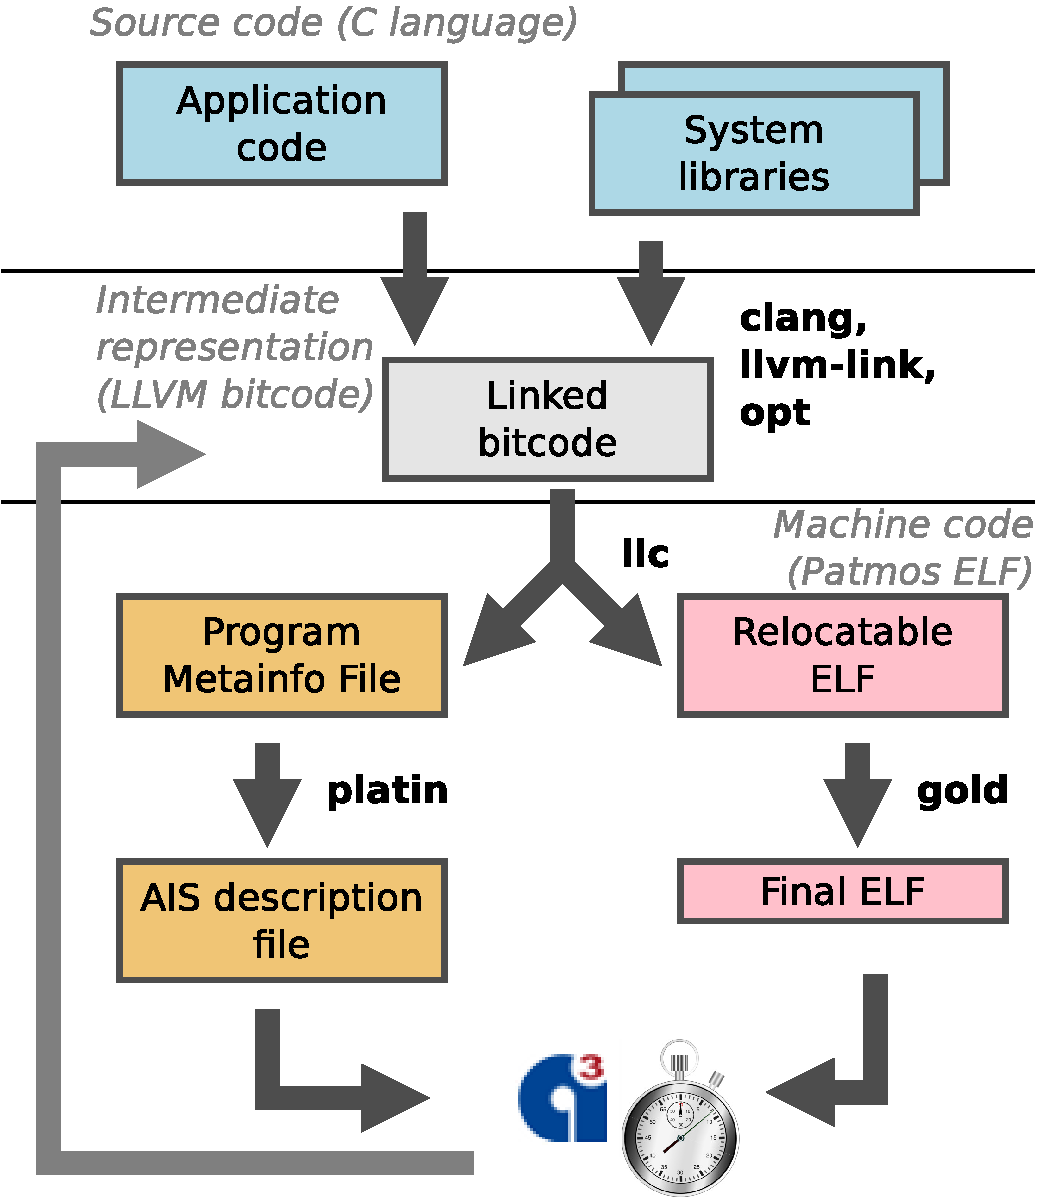
\includegraphics[width=0.5\textwidth]{fig/compiler_overview}
\caption{Compiler Tool Chain Overview}
\label{fig:compiler_overview}
\end{figure}


Figure~\ref{fig:compiler_overview} gives an overview of the compiler tool
chain.
The compilation process starts with the translation of each C source file and
libraries to the LLVM intermediate language (\emph{bitcode}) by the C frontend
\code{clang}. At this level, the user application code and static standard
and support libraries are linked by the \code{llvm-link} tool.
An advantage of linking on bitcode level is that subsequent analysis and
optimisation passes, and the code generation backend have a complete view of
the whole program. The \code{opt} optimiser performs generic,
target independent optimisations, such as common sub-expression elimination,
constant propagation, etc.

The \code{llc} tool constitutes the backend, translating LLVM bitcode into
machine code for the Patmos ISA, and addressing the target-specific features
for time predictability.  The backend produces a relocatable ELF binary
containing symbolic address information, which is processed by \code{gold}%
%
\footnote{gold is part of the GNU binutils, see
\url{http://sourceware.org/binutils/}}, defining the final data and memory
layout, and resolving symbol relocations.

In addition to the machine code, the backend exports supplementary information
for WCET analysis and optimisation purposes in form of a \emph{Patmos Metainfo
File}.  This information contains, among others, flow information (in form of
loop bounds provided by symbolic analysis on bitcode level), structural
information (targets of indirect branches), and information on memory accesses
(memory areas accessed by individual load/store instructions).
%
This information can be further processed by the \code{platin} toolkit, by
enhancing it (e.g., by a hardware model), translating it (e.g., to the input
format for annotations of the timing analysis tool \code{aiT}, as used in the
T-CREST project), or performing other analyses on it.





%%%%%%%%%%%%%%%%%%%%%%%%%%%%%%%%%%%%%%%%%%%%%%%%%%%%%%%%%%%%%%%%%%%%%%%%%%%%%%%
\section{Compiling with the \code{patmos-clang} Driver}

This section describes the usage of the \code{patmos-clang} C compiler.

\subsection{Compiling and Linking C Programs}

C source files are by default compiled to bitcode objects (\code{patmos-clang -c}). To compile .c files
to ELF objects, use \code{patmos-clang -c -fpatmos-emit-reloc}.

Assembly files are always compiled to ELF objects. Archive files (.a) can only contain bitcode objects
or ELF objects, not a mixture of both. Shared libraries (either bitcode or ELF) are not supported.

It is possible to link multiple bitcode files into a single bitcode file and link it like a static library
(compile with \code{patmos-clang -fpatmos-link-object -o lib<name>.bc}, link with -l<name>). Bitcode files are always
fully linked in, even if there is no usage of any of its symbols. Unused symbols are removed in a separate
optimization step.


\stefan{TODO Make the following a subsection. Describe interaction with platin, install directories layout of newlib. Show typical
compile commands using examples (compiling a single file, comiling a lib, compiling with platin,...}


\paragraph{Compiling single files to objects (using patmos-clang -c|-S)}

\begin{enumerate}
\item Input .c files are compiled to bitcode files by default. Use -fpatmos-emit-obj to compile
   to ELF objects, or -fpatmos-emit-asm to compile to assembly files.

\item Input .s files are compiled to ELF files.
\end{enumerate}


\paragraph{Linking multiple files with patmos-clang (i.e, not using -c or -S)}

The compiler driver (patmos-clang) performs the following steps to compile and link multiple input files.

\begin{enumerate}
\item All .c input files are compiled to individual bitcode objects. All assembly files are compiled to
   individual ELF files.

\item If -nostartfiles is not given and the target OS is not RTEMS, crt0 is added as first input file.

\item Depending on the -nodefaultlibs|-noruntimelibs|.. options, the following libraries are added
   after all user provided inputs: -lc (libc), -lpatmos (libgloss), -lrtsf (softfloats), -lrt (runtime).

\item For any of the above libraries, as well as -lm (libm), a lib<libname>syms.o file is added if the library
   is a bitcode library. The lib<x>syms.o files force the linker to pull in functions for which calls might be
   generated by LLC when compiling from bitcode to ELF.

\item All input files and libraries are checked if they are bitcode files/archives or ELF files/archives. All
   bitcode files are linked into a single bitcode file. ELF files are ignored in this step.

Attention: This means that symbols that are defined in bitcode archives but are used only in ELF input files
   are not linked in! You need to link in a separate bitcode file containing a pseudo use of the required symbols.

\item The resulting bitcode file is optimized and compiled to relocatable ELF.

Attention: The optimization step removes any symbol from the bitcode that are not used in bitcode.
   If a function is called only in an ELF object, you need to mark the function with \code{\_\_attribute\_\_((used))}.

\item The ELF file is linked with the other ELF files and ELF libraries at the position of the first bitcode input file.
   Relocations are resolved and additional symbols are defined. The result is an executable ELF file.

Attention: Since bitcode inputs are linked first in a separate step, the linking order between bitcode files
   and ELF inputs is not (yet) fully preserved. Using -flto does not solve this, since the LTO plugin also
   links all bitcode files first, and only links in the linked bitcode file *after* all ELF inputs!

\end{enumerate}

\subsubsection{Driver Options}

The \texttt{patmos-clang} driver can be used to generate bitcode files, to link bitcode files, or to 
emit assembler code. The driver supports the following modes of operation:

\begin{description}
\item[\texttt{patmos-clang -c <inputs>}] \hfill\\
  \begin{tabular}{ll}
  Input:   & \texttt{.c} C source file \\
  Output:  & \texttt{.o} or \texttt{.bc} bitcode files \\
  Actions: & compile each input file to a bitcode file
  \end{tabular}

\item[\texttt{patmos-clang -S <inputs>}] \hfill\\
  \begin{tabular}{ll}
  Input:   & \texttt{.c} C source file \\
  Output:  & \texttt{.s} or \texttt{.ll} human readable bitcode files \\
  Actions: & compile each input file to a human readable bitcode file
  \end{tabular}

\item[\texttt{patmos-clang -fpatmos-emit-llvm <inputs>}] \hfill\\
  \begin{tabular}{ll}
  Input:   & \texttt{.c} C source file, \texttt{.bc} bitcode object file, \texttt{.a} bitcode files archive \\
  Output:  & bitcode file \\
  Actions: & compile to bitcode, link all input files, link with standard libraries and start code \\
\end{tabular}

\item[\texttt{patmos-clang -fpatmos-emit-reloc -c <inputs>}] \hfill\\
  \begin{tabular}{ll}
  Input:   & \texttt{.c} C source file \\
  Output:  & \texttt{.o} Patmos relocatable ELF \\
  Actions: & compile each input file to a Patmos relocatable ELF file
  \end{tabular}

\item[\texttt{patmos-clang -fpatmos-emit-asm -S <inputs>}] \hfill\\
  \begin{tabular}{ll}
  Input:   & \texttt{.c} C source file \\
  Output:  & \texttt{.s} Patmos assembly file \\
  Actions: & compile each input file to a Patmos assembly file
  \end{tabular}

\item[\texttt{patmos-clang -fpatmos-emit-reloc <inputs>}] \hfill\\
  \begin{tabular}{ll}
  Input:   & \texttt{.c} C source file, \texttt{.bc} bitcode object file, \texttt{.a} bitcode files archive \\
  Output:  & \texttt{.o} Patmos relocatable ELF \\
  Actions: & compile to bitcode, link all input files, link with standard libraries and start code, \\
	   & compile to relocatable ELF
\end{tabular}

\item[\texttt{patmos-clang -fpatmos-emit-asm <inputs>}] \hfill\\
  \begin{tabular}{ll}
  Input:   & \texttt{.c} C source file, \texttt{.bc} bitcode object file, \texttt{.a} bitcode files archive \\
  Output:  & \texttt{.o} Patmos assembly file \\
  Actions: & compile to bitcode, link all input files, link with standard libraries and start code, \\
	   & compile to Patmos assembly
\end{tabular}

\item[\texttt{patmos-clang -o <output> <inputs>}] \hfill\\
  \begin{tabular}{ll}
  Input:   & \texttt{.c} C source file, \texttt{.bc} bitcode object file, \texttt{.a} bitcode files archive \\
  Output:  & Patmos executable ELF \\
  Actions: & compile to bitcode, link with standard libraries and start code, \\
           & compile to relocatable ELF, create Patmos executable ELF
  \end{tabular}

\end{description}

The compiler accepts standard options such as \texttt{-I}, \texttt{-L} and \texttt{-l} to define additional
lookup paths for header files and libraries and to link with (static) libraries.
The behaviour of the linker can be controlled with additional options for \texttt{patmos-clang} 
as shown in Table~\ref{tab:linker_options}.
Refer to \code{patmos-clang --help-hidden} for a list of all available options that control the behaviour of
the driver, and to \code{patmos-llc --help-hidden} for all options that control the generation of machine code from
bitcode. Options can be passed from \code{patmos-clang} to \code{patmos-llc} and other tools using \code{-Xclang},
\code{-Xopt}, \code{-Xllc}, \code{-Wl} and so on.
To pass options to the internal LLVM backend of the clang compiler, use \code{patmos-clang -Xclang -mllvm -Xclang
<option>}.

\begin{table}
\centering
\begin{tabular}{ll}
Option & Description \\ \hline
\texttt{-mfloat-abi=none} & Do not use software floating point libraries when linking \\
\texttt{-nostdlib} & Do not use standard libraries such as \texttt{libc} when linking \\
\texttt{-nolibc} & Do not use \texttt{libc} when linking \\
\texttt{-nodefaultlibs} & Do not use platform system libraries when linking\\
\texttt{-nostartfiles} & Do not use the \texttt{crt0} start file when linking \\
\texttt{-nolibsyms} & Do not use symbol definition files for runtime libraries when\\
                    & linking. Those files prevent the linker from removing any \\
		    & functions for which calls might be generated by the compiler \\
		    & backend, such as software division or \texttt{memcpy} \\
\texttt{-fpatmos-link-object} & Link as object, i.e., do not link in any libraries or start code 
\end{tabular}
\caption{Options for \texttt{patmos-clang} that control the default behaviour of the linker}
\label{tab:linker_options}
\end{table}

\subsubsection{Libraries}

The Patmos tool chain supports static libraries. Libraries are archives that contain
either only bitcode files or ELF objects. The archives are created by using either the \texttt{ar}
tool provided by the host system or by using \texttt{patmos-ar} from the \texttt{patmos-gold} binutils. The tool
\texttt{patmos-llvm-nm} can be used to inspect the content of bitcode archives.

\begin{verbatim}
ar q libtest.a *.bc
# show the contents of libtest.a
patmos-llvm-nm libtest.a
# compile and link with the created library
patmos-clang -target patmos-unknown-elf -o app main.c -ltest
\end{verbatim}


\subsection{Disassembling}

To disassemble .bc files, use \code{patmos-llvm-dis <file>.bc}.

To disassemble .o ELF files, use \code{patmos-llvm-objdump -d <file>}. Add '-r' to show relocation symbols
(for relocatable ELFs or executables generated with -Xgold -q).

\subsection{Debugging}

Some useful commands for debugging:

\begin{verbatim}
# print out executed instructions and the values of their operands
# starting from some cycle
pasim --debug=<cycle-to-start-printing> --debug-fmt=instr <binary>

# show disassembly of binary
patmos-llvm-objdump -r -d <binary> | less

# compile with debug infos, show source line numbers
patmos-clang -g -o <binary> ...
readelf --debug-dump=decodedline <binary>

# Compile with debugging info: use CFLAGS="-g" for your application, and add
# the following to your build.cfg:

NEWLIB_TARGET_CFLAGS="-g"
COMPILER_RT_CFLAGS="-g"

# Annotate objdump with source line numbes (this is quite slow at the moment)
patmos-llvm-objdump -r -d <binary> | patmos-dwarfdump <binary> | less

# Annotate simulation trace and stack-trace with line numbers
pasim --debug=<cycle-to-start-printing> --debug-fmt=instr <binary> 2>log.txt
cat log.txt | patmos-dwarfdump <binary>
\end{verbatim}

\subsection{Various options}

\paragraph{Keep relocation infos in executable for objdump:} (does not work with patmos-clang -g !)

\begin{verbatim}
patmos-clang -Xgold -q -o <binary> ....
patmos-llvm-objdump -r -d <binary> | less
\end{verbatim}




%%%%%%%%%%%%%%%%%%%%%%%%%%%%%%%%%%%%%%%%%%%%%%%%%%%%%%%%%%%%%%%%%%%%%%%%%%%%%%%
\section{\code{platin} -- The Portable LLVM Annotation and Timing Toolkit}
\label{sec:toolchain:platin}

The \code{platin} toolkit provides a set of useful tools to process the
information exported by the compiler in the PML format, with respect to
timing analysis integration.


The usage of \code{platin} is:

\begin{verbatim}
  platin <tool> <tool-options>
\end{verbatim}

You can get help on a particular tool with either of

\begin{verbatim}
  platin <tool> --help
  platin help <tool>
\end{verbatim}


Below we present a list of the most useful tools.

\begin{description}

  \item[pml2ais] \hfill\\
    Translates information of a PML file relevant to timing analysis to
    the AIS annotation format.

  \item[extract-symbols] \hfill\\
    The compiler exports program information at a stage where the final memory
    layout is not yet defined. This tool reads the final executable and
    enhances the PML file with information on the final addresses of
    instructions and data.

  \item[analyze-trace] \hfill\\
    Based on the structural information of a program in the PML file,
    the trace analysis tool is capable of extracting flow fact hypotheses
    based on a simulation run. These are context-sensitive and include,
    e.g.\ observed loop bounds and function call targets.

  \item[transform] \hfill\\
    Transforms flow facts from bitcode to machine code level
    or simplifies a set of flow facts.

  \item[tool-config] \hfill\\
    Given a hardware model (in PML format), this tool outputs consistent
    hardware configuration options/parameters for use during compilation,
    simulation and WCET analysis.

  \item[pml-config] \hfill\\
    Create and modify a hardware model in PML format based either on the 
    default configuration for a given target triple or on an existing PML
    hardware model. 

  \item[pml] \hfill\\
    Provides validation, inspection and merge facilities for PML files.

  \item[visualize] \hfill\\
    Visualises structural information of the program in the different program
    representations.

  \item[wcet] \hfill\\
    A driver that starts WCET analysis from the command line.

\end{description}


In addition to the platin tools, another command-line utility,
\texttt{patmos-clang-wcet}, is provided. This tool invokes the compiler
(\texttt{patmos-clang}), timing analysis, and the compiler a second time
(with intermediate calls to platin tools as necessary) for WCET-guided
optimisations based on timing-analysis feedback.
\daniel{TBD}

\subsection{The PML File Format}

\code{platin} stores all internal information and configuration in \emph{Platin Metainformation Language} (PML) files.
PML files are \emph{YAML} files that adhere to the PML schema. The schema file can be found in

\begin{verbatim}
patmos-llvm/tools/platin/lib/core/pml.yml
\end{verbatim}

\stefan{There is a tool to generate a HTML document out of it..}

Many \code{platin} tools accept multiple PML input files. Multiple PML files can also be merged using
the \code{pml} tool.

\subsection{PML Architecture- and Tool Configuration}

PML configuration files are used to set up tools such as the \code{pasim} or the
\code{clang} compiler via the \code{tool-config} tool, and provides timing and cache information to the WCET analyses.

Typically, the configuration is stored in a separate PML file that is passed to the \code{platin} tools as
additional input file using the \code{-i} option. Sample configuration files can be found in

\begin{verbatim}
patmos-llvm/tools/platin/etc/
\end{verbatim}
\stefan{Maybe we will install those files somewhere along with the .rb files.}




There are three configuration sections: 
\begin{itemize}
\item \code{machine-configuration}: The machine configuration defines memory size and timings, caches and memory areas.
  If no machine configuration is present, a default configuration will be used.
\item \code{tool-configurations}: This section contains additional tool configurations and options.
\item \code{analysis-configurations}: The analysis section sets up one or more WCET analyses. This section is currently work in progress.
\end{itemize}

\paragraph{The \code{machine-configuration} Section}


% TODO make this a figure or something. Maybe shorten?
\begin{verbatim}
---
format: pml-0.1
triple: patmos-unknown-unknown-elf
machine-configuration:
  memories:
    - name: "main"
      size: 0x200000
      transfer-size: 16
      read-latency: 3
      read-transfer-time: 4
      write-latency: 3
      write-transfer-time: 4
    - name: "local"
      size: 2048
      transfer-size: 4
      read-latency: 0
      read-transfer-time: 0
      write-latency: 0
      write-transfer-time: 0
  caches:
    - name: "data-cache"
      block-size: 16
      associativity: 1
      size: 2048
      policy: "lru"
      type: "set-associative"
    - name: "method-cache"
      block-size: 8
      associativity: 16
      size: 4096
      policy: "fifo"
      type: "method-cache"
    - name: "stack-cache"
      block-size: 4
      size: 2048
      type: "stack-cache"
  memory-areas:
    - name: "code"
      type: "code"
      memory: "main"
      cache: "method-cache"
      address-range:
        min: 0
        max: 0x200000
    - name: "data"
      type: "data"
      memory: "main"
      cache: "data-cache"
      address-range:
        min: 0
        max: 0x200000
      attributes:
        - key: "heap-end"
          value: 0x100000
        - key: "stack-base"
          value: 0x200000
        - key: "shadow-stack-base"
          value: 0x1f8000
\end{verbatim}


The machine configuration consists of three sections:
\begin{itemize}
\item \code{memories}: This section specifies the available memories and their timings. Each entry must define
  the following properties of the memory:

  \begin{itemize}
  \item \code{name}: The (unique) name of the memory.
  \item \code{size}: The size of the memory in bytes. Can be a hexadecimal value.
  \item \code{transfer-size}: The size of a single beat in bytes. Also defines the alignment of the memory.

  \stefan{This should actually be more like the bus width and in bits, but this has historic reasons..}
  \stefan{The alignment should be a separate attribute, could be between transfer size and min-burst-size.}

  \item \code{min-burst-size}: The minimum size of a single burst in bytes. Defaults to \code{transfer-size}.
  \item \code{max-burst-size}: The maximum size of a single burst in bytes. Defaults to \code{min-burst-size}.
  
  \item \code{read-latency}: The latency per read \emph{request} in cycles.
  \item \code{read-transfer-time}: The number of cycles to read a single beat of size \code{transfer-size}.
  \item \code{write-latency}: The latency per write \emph{request} in cycles.
  \item \code{write-transfer-time}: The number of cycles to write a single beat of size \code{transfer-size}.
  \end{itemize}

  The number of cycles for a single, \code{max-burst-size}-aligned read or write request of $B$ bytes is 
  \[
  t_{req} = \left\lceil \frac{\max(B, \texttt{min-burst-size})}{\texttt{max-burst-size}}\right\rceil \cdot \texttt{latency} +
            \left\lceil \frac{\max(B, \texttt{min-burst-size})}{\texttt{transfer-size}}\right\rceil \cdot \texttt{transfer-time}
  \]
  For unaligned requests that span over a single burst, the transfer time can increase by up to $\texttt{latency} + \texttt{transfer-time}$.

  \textbf{Ideal memory:} A memory is \emph{ideal}, if all latency and transfer time delays are set to zero.

  \begin{framed}
  \textbf{Patmos:} For a Patmos machine configuration, there must be exactly one memory named \texttt{main}. This memory configuration is used to setup
    the global memory. If \texttt{main} does not exist, an ideal memory is assumed.

    The memory configuration named \texttt{local} is used to setup the local scratchpad memory. Currently, the local memory must be
    an ideal memory.

    All other memory configurations are \emph{ignored}.
  \end{framed}

\item \code{caches}: This section defines all caches of the core. Each entry must define the following properties:
  
  \begin{itemize}
  \item \code{name}: The (unique) name of the cache.
  \item \code{type}: The cache type. Supported values are \code{none}, \code{set-associative}, \code{method-cache} and \code{stack-cache}.
  If set to \code{none}, the cache is disabled. This is equivalent to this cache's section not being present.
  \item \code{policy}: The replacement policy of the cache. Supported values are \code{ideal}, \code{lru} and
    \code{fifo} for a method cache or a set-associative cache. For set-associative caches, the policy \code{dm} (direct
    mapped) is also supported. For a stack cache, supported values are \code{ideal}, \code{block}, \code{lblock},
    \code{ablock} and \code{dcache}.
    An ideal cache will always hit. In particular, it does \emph{not} have cold misses. In order to simulate an ideal
    cache with cold misses, setup a very large fully associative cache (a very large direct mapped data cache is ideal for
    the simulation, but not ideal for the analysis as it is not resilient against unknown accesses).
  \item \code{associativity}: Defines the associativity of a \code{lru} or \code{fifo} set-associative cache, or the 
    tag memory size for a method cache. Ignored for all other types of caches.
  \item \code{size}: The size of the cache in bytes. Ignored for ideal caches.
  \item \code{block-size}: The size of a cache line for set-associative caches, or the internal alignment of cache
    blocks for stack caches and method caches, in bytes. A block size of $4$ (or less) corresponds to a
    variable-sized method cache. A block size of $\texttt{size}/\texttt{associativity}$ corresponds to a fixed-size
    method cache. For set-associative caches, the block size will typically be the same as the underlying memory 
    transfer size. 

    At the moment, the block-size is always required to be set.
  \item \code{attributes}: A list of additional attributes as \code{key} and \code{value} pairs.
  \end{itemize}

  \begin{framed}
  \textbf{Patmos:} Patmos supports the following cache names: \code{data-cache}, \code{stack-cache}, \code{method-cache} and 
    \code{instruction-cache}. All other caches are \emph{ignored}.
    
    The \code{data-cache} must be a set-associative cache.
    The \code{stack-cache} must be of type \code{stack-cache}. If a data cache but no stack cache is configured,
    requests to the stack cache will be handled through the data cache.
    The \code{method-cache} must be a method cache.
    The \code{instruction-cache} must be a set-associative cache.

    It only allowed to specify both a \code{method-cache} and an \code{instruction-cache} if at least one of them has
    the type set to \code{none}.

    The \code{platin pml-config} tool can be used to easily switch between a method-cache and an instruction-cache 
    configuration. It will automatically set the correct types and link the caches to the memory areas. 

    \stefan{I would rather like to see a single 'instruction-cache' entry with either set-assoc or method-cache as type,
    to avoid a few consistency checks, but maybe there could be a configuration possible in the future which has both types of
    caches (at least in the simulator).}

    \emph{Attention:} If an ideal data cache is configured, all \emph{stores} through the data cache also have a zero-cycle
    latency, but bypass loads (and bypass stores) are unaffected.
    Bypass loads and stores only have a zero-cycle latency if the \code{main} memory is configured as ideal memory. In
    this case, all data and code accesses have zero latency, regardless of the configured caches.
  \end{framed}

\item \code{memory-areas}: The memory areas set up a mapping of address ranges to memories
  and define the caches that are used for those address ranges and access types. Each mapping must define the following
  properties:

  \begin{itemize}
  \item \code{name}: The (unique) name of the cache.
  \item \code{type}: The type of the contained data, must be one of \code{code} or \code{data}.
  \item \code{cache}: The name of the cache that is used for this address range and type of data.
  \item \code{memory}: The name of the memory of this address range is mapped to.
  \item \code{address-range}: The start (inclusive) and the end (exclusive) of the address range as property \code{min} and \code{max}.
    Defaults to $0$ to the size of the backing memory if omitted.
  \item \code{address-space}: The name of the address space. Defaults to \code{global}.
  \item \code{attributes}: A list of additional attributes as \code{key} and \code{value} pairs.
  \end{itemize}
  
  \begin{framed}
  \textbf{Patmos:} The address space must be either \code{global} or \code{local}. Local address space entries must not
  use a cache, and must use an ideal memory.

  Patmos supports the following named address spaces: 
  
  \begin{itemize}
  \item \code{code}: The main code area for regular instruction fetches. It must be of type \code{code}, use global address space, and refer to
                     \code{main} memory or an ideal memory. It must use either the \code{method-cache} or the \code{instruction-cache} such
		     a cache is defined (with a type different than \code{none}).
  \item \code{data}: The main data area for data and stack accesses. It must be of type \code{data}, use global address space, and refer to
                     \code{main} memory. It must use the \code{data-cache} if such a cache is defined. This area may
		     only use an ideal memory if the \code{main} memory is ideal.
  \end{itemize}

  All other code areas are currently ignored. If any of the above address spaces is omitted, \code{main} memory is used
  by default.

  \stefan{We might define additional area names in the future to configure the scratchpads. Maybe we should define a
  memory area called 'stack' and link it with the stack cache, or allow a list of names for the \code{cache} attribute.}

  The following attributes are supported: \code{heap-end} sets the heap end pointer, \code{stack-base} sets the stack
  base pointer, and \code{shadow-stack-base} sets the shadow stack base pointer. Those attributes can be defined in
  any memory area, but must be defined at most once.
  \end{framed}

\end{itemize}


\paragraph{The \code{tool-configurations} Section}

This section can be used to specify additional command line options or configuration values for various tools.

\begin{verbatim}
tool-configurations:
  - name: "clang"
    options: ["-mpatmos-disable-vliw"]
\end{verbatim}

The section contains a list of tool configurations, consisting of the following entries:
\begin{itemize}
\item \code{name} (required): The name of the tool to configure. Corresponds to \code{tool-config -t}. Currently supported
  tools are \code{clang}, \code{pasim} and \code{ait}. 
  % See the tool-config section .. if there would be anything interesting there.
\item \code{options}: A list of command line options that should be passed to the tool when configured via \code{tool-config} or 
  when called internally. Note that if you want to pass multiple options, the options must be specified as a YAML list, not as a 
  single string, in order to be quoted correctly.
\item \code{configuration}: A list of entries with \code{key} and \code{value}, specifying additional tool configuration values.
  The names of the keys are tool dependent. 
  Currently this is not used by any tool.
\end{itemize}

\paragraph{The \code{analysis-configurations} Section}

The analysis configuration is intended to set up one or more WCET analysis variants, either for 
multiple analysis targets, or for analysing with multiple scenarios or analysis configurations.
For each named analysis, a program entry point, a (WCET) analysis entry point, as well as additional tool configurations
per analysis can be specified.

\emph{Attention:} This section is currently work in progress and is only used to configure clang, but not the WCET analyses.


\subsection{Generating PML configurations}

It is possible to generate or modify PML hardware models using \code{platin pml-config}.

\begin{verbatim}
platin pml-config --target patmos-unknown-unknown-elf -o config.pml -m 2k \
                  --set-cache-attr method-cache,max-subfunction-size,1024 \
                  --set-area-attr data,heap-end,0x18000
\end{verbatim}

This creates a new default configuration and sets the method cache size to 2 kB and defines (or redefines) some
attributes. The result is stored in \code{config.pml}. It is also possible to print the result to stdout using 
\code{-o -}.

It is also possible to modify an existing configuration. This command takes the previously generated PML file,
disables the method cache and creates a new instruction cache entry (with default values) and sets its size to 8 kB
(without changing the disable method-cache entry). The result is written to stdout.

\begin{verbatim}
platin pml-config -i config.pml -o - -C icache -m 8k
\end{verbatim}

\emph{Attention:} At the moment \code{pml-config} is the only tool that includes a hardware model in its PML output.
All other tools will \emph{skip} any configuration section in its output. It is thus necessary to always explicitly pass
the configuration to platin, i.e., the following will not work as expected

\begin{verbatim}
platin pml -o merged.pml -i config.pml -i myprogram.pml
platin wcet -b myprogram -i merged.pml   # This uses a default configuration!
\end{verbatim}

because the merged file will not contain the configuration sections. Instead, the second command in this example also
needs the additional \code{-i config.pml} argument. This is because \code{patmos-llvm} currently does
not support importing PML files containing configuration sections, and may change in the future.

\stefan{We need to extend the PML.h file to support the full configuration structure. Alternatively, we could add
an option to \code{platin pml} that removes all config sections. Even if patmos-llvm can read the config sections,
it will probably not use the configurations to setup the optimization passes, because this is a bit tricky to get
right (there can be multiple configurations in the pml file, and how do we handle conflicts with commandline options?).}

\subsection{Exporting PML Metainfo During Compilation}

To obtain PML files, the \code{patmos-clang} driver needs to be invoked with

\begin{verbatim}
  patmos-clang -mserialize=<pml-file> [-mserialize-roots=<functions>] ...
\end{verbatim}

The option argument \code{<pml-file>} is the filename of the PML file that is
generated.

The option argument \code{<functions>} is a comma-separated list of function
names to which the exporting of Metainformation should be restricted.
Note that inlining should be prevented for those functions (see
Section~\ref{sec:toolchain:frontend}), otherwise they might be inlined and removed.
By default, information for all functions reachable from main is exported.


\subsection{Obtaining AIS Annotations}

The \code{aiT} timing analysis tool supports annotations in the form of
AIS files.
To generate a AIS annotation file from a PML metainfo file, the
\code{platin pml2ais} tool is used:

\begin{verbatim}
  platin pml2ais  --ais <output.ais>  <input.pml>
\end{verbatim}


\subsection{Exporting Loop Bounds}

Loop bounds obtained by the \emph{LLVM scalar evolution (SCEV)} analysis
on bitcode are exported as meta information.
%
To be usable as flow facts for WCET analysis, they must be resolved and
transformed to machine-code level:

\begin{verbatim}
  platin transform --transform-action=down --flow-fact-output=<name> \
            --analysis-entry=<func> -i <input.pml> -o <output.pml>
\end{verbatim}

where \code{<name>} is a name for the newly generated flow facts
\code{<func>} is the entry function enclosing the program points referred by
the flow facts (\emph{main} by default).
%
\code{<output.pml>} and \code{<input.pml>} can be identical.


\daniel{TODO: other tools and useful usage examples}

%%%%%%%%%%%%%%%%%%%%%%%%%%%%%%%%%%%%%%%%%%%%%%%%%%%%%%%%%%%%%%%%%%%%%%%%%%%%%%%
\section{Patmos-clang C Frontend}
\label{sec:toolchain:frontend}

\subsection{Inlining, Function Attributes}

In contrast to GCC and the clang C frontend, LLVM by design attaches function attributes to
function \emph{definitions only}, not to function declarations or function types.
It is thus not possible to attach function attributes at call sites or for external functions.
Function attributes \emph{must} be defined in the same unit as the definition, otherwise they
are silently discarded by the compiler.

\paragraph{Inlining functions}
The compiler follows the C99 rules for inlining. See here for an explanation:
%
\url{http://www.greenend.org.uk/rjk/tech/inline.html}

If a function is marked with \code{inline} only, it will not be emitted into the linked binary.
Thus, to mark functions as inline functions you must do one of the following:

\begin{itemize}
\item If the function is only used within one module, mark it as \code{static inline}.
The function will not be visible outside the module, like all static functions. The compiler will emit the 
function into the module if it is used.

\begin{verbatim}
static inline void foo(int n) {
    ...
}
\end{verbatim}

\item If the function should be used in several functions, define it 'inline' everywhere,
  and add a declaration or definition with 'extern inline' in exactly one module.

\begin{verbatim}
extern inline void foo(int n);

inline void foo(int n) {
    ...
}
\end{verbatim}
\end{itemize}

\paragraph{Prevent Inlining}
To prevent the compiler from inlining, use the noinline attribute.

\begin{verbatim}
void foo(int n) __attribute__((noinline));
void foo(int n) {
    ...
}
\end{verbatim}

Note that function attributes are attached to function definitions only, as mentioned above.
It is currently not possible to prevent function inlining at the call site itself.
The only way to prevent inlining for specific functions is to either define them \code{noinline}
at their \emph{definition}, or to make the call an inline asm call. 
However, at the moment inline asm is currently not supported by the platin analysis tools. 

\stefan{It is comparatively easy to add support though, the assembly parser can be invoked
in the LLVM backend on InlineAsm instructions and used to find and export inline asm calls.}

\paragraph{Marking Functions as Used}
To prevent the compiler from removing functions that have no call site in the bitcode
(either because they are entry functions or because the compiler generates the calls),
add the 'used' attribute to the function declaration.

\begin{verbatim}
void _start(void) __attribute__((used));
void _start(void) {
    ...
}
\end{verbatim}

Note that if the function is part of a module that is linked in from a bitcode archive,
the compiler will not link in the module if there is no usage of the function, even if it
is marked as used. To force the linker to link in functions from archives, add a declaration
for that function in any of your used modules, or link a bitcode module just containing declarations
for those functions before linking with the library.


\subsection{Target Triples and Target Identification}

The Patmos tool-chain supports to following target triples:

\begin{verbatim}
    patmos-unknown-unknown-elf      Do not use an OS, start with main() on bare metal
    patmos-unknown-rtems            Compile and link for RTEMS
\end{verbatim}

The C frontend defines the following macros for Patmos targets

\begin{verbatim}
    __PATMOS__
    __patmos__
\end{verbatim}

For RTEMS, the following macros are also defined:

\begin{verbatim}
    __rtems__
\end{verbatim}

Use the following command to get a list of all defines for a target (do not omit \code{-triple}):

\begin{verbatim}
    patmos-clang -cc1 -triple patmos-unknown-unknown-elf -E -dM </dev/null
\end{verbatim}

The default target triple for patmos-clang (without -cc1!) is \code{patmos-unknown-unknown-elf},
if the program is called \code{patmos-clang}. Otherwise, if the binary is called
\code{<target>-clang}, then \code{<target>} is used as default target triple if it is a valid triple.
Otherwise, the host architecture (defined at configure time) will be used.


\subsection{Inline Assembler}

Inline assembly syntax is similar to GCC inline assembly. It uses \%0, \%1, ... as placeholders for
operands. Accepted register constraints are: \code{r} or \code{R} for any general purpose register,
\code{\{\$<registername>\}} to use a specific register, \code{i} for immediates, or the index of an output register to
assign an input register the same register as the output register.

Example:
\begin{verbatim}
    int i, j, k;
    asm("mov  $r31 = %1  # copy i into r31\n\t"
        "add  %0 = $r5, %2\n\t"
        "call %3\n\t"        // call myfunction
        "nop ; nop \n\t"     // delay slots
        : "=r" (j)
        : "0" (i), "{$r10}" (k), "i" (&myfunction)
        : "$r5" );
\end{verbatim}

Please see Section \ref{sec:toolchain:backend} for a description of the Patmos assembler syntax.

\subsection{Naked Functions}

You can mark functions as naked to prevent the generation of a prologue, epilogue or any spill code.
In such functions, effectively only inline assembly is allowed. It is possible to use simple C code in naked 
functions, as long as the compiler does not need to spill registers. Note that the amount of spills generated by
the compiler depends on the optimization settings, i.e., naked functions containing C code might not compile at
\code{-O0}. In particular, life ranges of variables must not extend over basic blocks, over calls or over
inline assembly code.

Note that the compiler might choose to inline functions into naked functions. To prevent this, put your C code into a
separate function that is marked as \code{noinline}, and only call this function from the naked function.

The the time of writing, the compiler automatically inserts a return instruction in naked functions. This behavior might be changed
in the future, i.e., naked functions should either contain an explicit return statement or a \code{RET} instruction in
the inline assembler whenever the control flow reaches the end of the function.

\begin{verbatim}
void foo(int n) __attribute__((naked));
void foo(int n) {
    asm("nop");
}
\end{verbatim}


\subsection{Patmos Specific IO Functions}

The following header define functions to read out the CPU ID, the clock counter and the real-time clock (RTC), as well as to
interface with the UART and to setup exception and interrupt handler.

\begin{verbatim}
#include <machine/patmos.h>
#include <machine/uart.h>
#include <machine/exceptions.h>
\end{verbatim}

Please refer to the headers in \code{patmos-newlib/newlib/libc/machine/patmos/machine/} for documentation for now.


\subsection{Scratchpad Memory}

Use the following header to get the relevant functions and macros:

\begin{verbatim}
#include <machine/spm.h>
\end{verbatim}

The \code{\_SPM} macro must be used for all pointers that point into the SPM.

\begin{verbatim}
_SPM unsigned int *spm_data = (_SPM unsigned int*) 0x1234;
\end{verbatim}

You can use the \code{spm\_copy\_from\_ext} and \code{spm\_copy\_to\_ext} functions
to copy data from global memory to SPM and back. Use \code{spm\_wait()} to
wait for the copy transaction to complete.\footnote{At the moment memory copy is
performed by the processor and is a blocking function. In future versions of Patmos
this might be delegated to a DMA and then the wait function might be needed.}

\martin{However, the way as it is used in \code{spm\_memmove} with one wait
for several copies will not work. Not more than one outstanding copy.}


\stefan{TODO more on SPM? Refer to examples}

\subsection{Placing Functions into the Instruction Scratchpad}

Functions that should be placed into and executed from the instruction scratchpad must be placed at
a specific address range (see Table~\ref{tab:gmmap}). This can be achieved by assigning such functions
to a different segment in the ELF objects, and then instructing the linker to place these segments at
a different address.

Functions can be assigned to a segment using the following attribute.

\begin{verbatim}
void foo(int i) __attribute__((section(".text.spm")));
void foo(int i) {
    ...
}
\end{verbatim}

While the section name can be arbitrary, it should start with \code{.text.} so that functions are placed
into the text segment by default. The \code{.text.spm} segment name is used by some functions in 
\code{patmos-newlib}.

By default, any \code{.text.*} section will be linked in at the end of the text segment in the executable binary.
In order to define the address of the section, a linker script must be used and provided at the linking stage.
Such a linker script is provided in \code{patmos/hardware/spm\_ram.t}.

\begin{verbatim}
SECTIONS
{
  . = SEGMENT_START(".rodata", 0x400);
  .rodata : { *(.rodata .rodata.*) }
  .init_array : { *(SORT(.init_array.*) .init_array) }
  .fini_array : { *(SORT(.fini_array.*) .fini_array) }
  .data : { *(.data) }
  .bss : { *(.bss) }

  . = ALIGN(8);
  _end = .; PROVIDE (end = .);

  . = SEGMENT_START(".text.spm", 0x10000);
  .text.spm : { *(.text.spm) }

  . = SEGMENT_START(".text", 0x20000);
  .text : { *(.text .text.* ) }

}
\end{verbatim}

The linker script must then be passed to the linker.

\begin{verbatim}
patmos-clang -Xgold -T -Xgold path/to/spm_ram.t -o hello hello.o
\end{verbatim}

Note that the instruction scratchpad is currently not available in the multicore version of Patmos.

\stefan{TODO some words about how the code actually gets into the I-SPM (bootloader??).}


%\subsection{Source Flow Annotations}
%
%TODO currently not implemented



%%%%%%%%%%%%%%%%%%%%%%%%%%%%%%%%%%%%%%%%%%%%%%%%%%%%%%%%%%%%%%%%%%%%%%%%%%%%%%%
\section{Patmos Compiler Backend}
\label{sec:toolchain:backend}

\subsection{ELF File Format}

\paragraph{ELF Identification:}

\begin{verbatim}
e_machine: EM_PATMOS = 0xBEEB
\end{verbatim}

\paragraph{ELF Relocation infos:}
Table~\ref{tab:elfrelocs} shows the ELF relocation types.

\begin{table}
  \centering
  \begin{tabular}{lll}
    \toprule
    Name & Value & Description \\
    \midrule
\texttt{R\_PATMOS\_NONE}         & 0  & no relocation \\
\texttt{R\_PATMOS\_CFLB\_ABS}    & 1  & CFLb format (22 bit immediate), absolute (unsigned), in words \\
\texttt{R\_PATMOS\_CFLB\_PCREL}  & 2  & CFLb format (22 bit immediate), PC relative (signed), in words \\
\texttt{R\_PATMOS\_ALUI\_ABS}    & 3  & ALIi format (12 bit immediate), absolute (unsigned), in bytes \\
\texttt{R\_PATMOS\_ALUI\_PCREL}  & 4  & ALUi format (12 bit immediate), PC relative (signed), in bytes \\
\texttt{R\_PATMOS\_ALUL\_ABS}    & 5  & ALUl format (32 bti immediate), absolute (unsigned), in bytes \\
\texttt{R\_PATMOS\_ALUL\_PCREL}  & 6  & ALUl format (32 bit immediate), PC relative (signed), in bytes \\
\texttt{R\_PATMOS\_MEMB\_ABS}    & 7  & LDT or STT format (7 bit immediate), signed, in bytes \\
\texttt{R\_PATMOS\_MEMH\_ABS}    & 8  & LDT or STT format (7 bit immediate), signed, in half-words \\
\texttt{R\_PATMOS\_MEMW\_ABS}    & 9  & LDT or STT format (7 bit immediate), signed, in words \\
\texttt{R\_PATMOS\_ABS\_32}      & 10 & 32 bit word, absolute (unsigned), in bytes \\
\texttt{R\_PATMOS\_PCREL\_32}    & 11 & 32 bit word, PC relative (signed), in bytes \\
    \bottomrule    
  \end{tabular}
  \caption{ELF relocation types}
  \label{tab:elfrelocs}
\end{table}

\stefan{make a table out of this}

\paragraph{Subfunctions, Symbols:}

\begin{itemize}
\item ELF Symbol flags:
  \begin{itemize}
  \item \code{MCSA\_ELF\_TypeCode} / \code{STT\_CODE} (value 13): set for symbols which point to the beginning of a (sub) function
      (i.e., the first instruction after the alignment and function size word)
  \end{itemize}
\item Function symbol points to first instruction of function, has \code{.type function}, \code{.size} is whole function size
\item Code symbol points to first instruction of subfunction, has \code{.type code}, \code{.size} is size of subfunction
\item The first subfunction of a function only has a function symbol, following subfunctions have a code symbol (i.e.,
  the size value for the first subfunction in the symbol is not the same as the actual size)
\end{itemize}

\subsection{LLVM backend fixups, symbols, immediates}

At MC level, immediates are always in byte/half-word/word as the instruction where they are used,
i.e., immediates are already properly shifted.

The assembler parser and assembler printer (i.e., the disassember and .s emitter) parse and print
immedates without conversion, i.e., immediates are printed in words/half-words/bytes, depending on
the instruction. 


\subsection{Assembler Syntax}

This section describes the assembler syntax of the LLVM assembler parser and printer, as well as the inline assembler.

Note that the \code{paasm} assembler provided with Patmos has a slightly different syntax, i.e., opcode mnemonics
have suffixes, the syntax for bundles is different, and only a very limited set of directives is accepted by \code{paasm}.

\paragraph{General Instruction Syntax:}

Each operation is predicated, the predicate register is specified before the operation in
parentheses, e.g. \code{(p1) <instruction>}.  If the predicate register is prefixed by a \code{!}, it is negated.
If omitted, the predicate defaults \code{(p0)}, i.e., always true.

All register names must be prefixed by \$. The instructions use destination before source in the
instructions. Between destination and source a \code{=} character must be used instead of a comma.

Immediate values are not prefixed for decimal notation, the usual 0 and 0x formats are accepted for
octal and hexadecimal immediates. Comments start with the hash symbol \code{\#} and are considered to the
end of the line.

For memory operations, the syntax is \code{[\$register + offset]}. Register or offset can be ommited, in
that case the zero register \code{r0} or an offset of $0$ is used.

Labels that are prefixed by .L are local labels. Labels may only appear between bundles, not inside bundles.

Example:
\begin{verbatim}
    # add 42 to contents of r2
    # and store result in r1 (first slot)
    { add   $r1 = $r2, $42
    # if r3 equals 50, set p1 to true
    cmpeq $p1, $r3, 50 }
    # if p1 is true, jump to label_1
    ($p1) br .Llabel1 ; nop ; nop   # then wait 2 cycles
    # Load the address of a symbol into r2
    li $r2 = .L.str2
    # perform a memory store and a pred op
    { swc [$r31 + 2] = $r3 ; or $p1 = !$p2, $p3 }
    ...
.Llabel1:
    ...
\end{verbatim}


\paragraph{Bundles:}
A semi-colon \code{;} or a newline denotes the end of an instruction or operation. If an instruction contains
two operations, the operations in the bundle must be enclosed by curly brackets. For bundles consisting
only of one operation, the brackets are optional.

Known bugs:
The closing bracket must appear on the same line as the last operation in the bundle. The opening bracket might
be followed by a newline, but no comments or labels may appear between the bracket and the first operation.


\paragraph{Function Block Start Markers and Subfunction Calls:}
Functions must be prepended by the \code{.fstart} directive which emits the function size word and aligns the
code.

\begin{verbatim}
    .fstart <label>, <size-in-bytes>, <alignment-in-bytes>
\end{verbatim}

The alignment must be a power of 2. The function size must be the size of the following (sub-)function.
If a function is split into several subfunctions, the size must be the size of the first sub-function,
not the size of the whole function (this differs from the .size directive).

\begin{verbatim}
    .type   foo,@function
    .size   foo, .Ltmp2-foo         # size of foo symbol is the whole function
    .fstart foo, .Ltmp0-foo, 4
foo:                                # start of foo function
    sres  10
    ...
    brcf .Ltmp1                     # Fallthrough to different subfunction is not allowed
    nop
    nop
    nop
.Ltmp0:                             # end of first subfunction of foo

    .type   .Ltmp1,@code
    .size   .Ltmp1, .Ltmp2-.Ltmp1
    .fstart .Ltmp1, .Ltmp2-.Ltmp1, 4
.Ltmp1:                             # start of second subfunction of foo
    ...
    ret $r30, $r31                  # returns from foo, not from the subfunction
    nop
    nop
    nop
.Ltmp2:                             # end of (second subfunction of) foo
\end{verbatim}

To set the address of a function relative to the start of the section, use the .org directive before
the .fstart directive and allow for the function size word so that .fstart does not emit any padding.

\begin{verbatim}
    .org <aligned startaddress>-4
    .fstart .foo, .Ltmp0-.foo, <alignment>
foo:
    ....
\end{verbatim}

\subsection{Address Spaces}

Set address space of a pointer by using \code{\_\_attribute\_\_((address\_space(<nr>)))}. See \code{patmos.h} in newlib.

Used address spaces:
\begin{itemize}
\item Address Space 0 (default): main memory with data cache
  \begin{itemize}
  \item nontemporal flag: main memory with bypass
      Set only by the compiler (at the moment)
  \end{itemize}
\item Address Space 1: (local) scratchpad memory
  \begin{itemize}
  \item use macro \code{\_SPM} defined in \code{<machine/spm.h>} for SPM accesses
  \item use macro \code{\_IODEV} defined in \code{<machine/patmos.h>} to access memory mapped IO devices
  \end{itemize}
\item Address Space 2: Stack cache
  \begin{itemize}
  \item Compiler-maintained, must not be used in application code (at the moment)
  \end{itemize}
\item Address Space 3: main memory without data cache
  \begin{itemize}
  \item use macro \code{\_UNCACHED} defined in \code{<machine/patmos.h>}
  \end{itemize}
\end{itemize}

%%%%%%%%%%%%%%%%%%%%%%%%%%%%%%%%%%%%%%%%%%%%%%%%%%%%%%%%%%%%%%%%%%%%%%%%%%%%%%%
\section{Newlib}

The Patmos compiler contains a port of newlib, a C library intended for embedded systems. When  writing
downloadable applications it is suggested to use newlib functions instead of the low-level functions provided
by Patmos specific IO functions.\footnote{Those functions are mainly used to write very small footprint programs,
such as the bootloader itself.}

Documentation of the provided newlib library and available functions is available at:

\url{https://sourceware.org/newlib/}

%%%%%%%%%%%%%%%%%%%%%%%%%%%%%%%%%%%%%%%%%%%%%%%%%%%%%%%%%%%%%%%%%%%%%%%%%%%%%%%
\section{Known Bugs, Restrictions and Common Issues}
\label{sec:toolchain:knownbugs}


\paragraph{Undefined reference to <libc function>:} Some LLVM passes might create calls to standard library functions
after the bitcode linking phase. We added all such functions that we found to \code{libcsyms.ll.in} in \code{compiler-rt}.
If we missed some functions, they must be added. Alternatively, newlib and compiler-rt could be compiled as ELF libraries.

It could also be the case that newlib needs to be recompiled, or that your linking order is wrong (be aware
that mixing bitcode or C files, assembly files and ELF files causes the linking order to be changed).


\paragraph{Inline assembler:} Clobbering the registers \code{\$r30/\$r31} is not supported and calls inside
inline assembler will not cause the prologue to save \code{\$r30/\$31}. Do not modify them in inline assembly.


\paragraph{Inline assembler:} Constraining an output to a register (\code{"={\$r10}"}) does not work, for some reason
LLVM looses the output register operand somewhere between \code{SelectionDAGBuilder::visitInlineAsm()} and
\code{AsmPrinter::EmitInlineAsm()}.


\paragraph{C code in \code{\_\_naked\_\_} functions:} Writing C code statements in naked functions might cause
the compiler to spill registers (be aware that the compiler will spill much more registers at \code{-O0}!). 
This is not supported since naked function do not have a prologue or epilogue setting up the stack frame.


\paragraph{patmos-\{objdump,objcopy,..\} does not support Patmos ELF files:} Only patmos-ld supports the Patmos
ELF file type. patmos-ar and patmos-nm have some support for bitcode archives (when the LLVMgold plugin is
compiled, default for build.sh builds). Other binutils tools have no support for Patmos ELFs.
Use \code{patmos-llvm-objdump} and \code{patmos-ld} instead.


\paragraph{Compiling patmos-gold with GCC 4.7.0 aborts with an error about narrowing conversion:}
Workaround: use CXXFLAGS=-Wno-narrowing for configure, upgrade to a newer GCC version or
use clang to compile the toolchain.

If you are using the build.sh script, set \code{GOLD\_CXXFLAGS="-Wno-narrowing"} in \code{build.cfg}.


\paragraph{Keeping relocations in the executable (-Xgold -q) and debugging info (-g) do not work together:}
This seems to be a gold restriction.





% % % % % % % % % % % % % % % % % % % % % % % % % % % % % % % % % % % % % % % %
\chapter{Potential Extensions}

\section{Multiply / Wait / Move from Special}

\begin{itemize}
  \item Attaching a ready flag with all special registers.
  \item Specify destination special register with all decoupled operations; the
        operation sets/resets the ready flag accordingly.
  \item Wait operates on ready flags of special registers.
  \item Merged variant of Wait + Move from Special
  \item Wait with 16-bit mask to wait for multiple outstanding results.
\end{itemize}

This would be nice since it would allow to reload all special registers from
memory without going through the general purpose registers. It would be a
unified interface for decoupled operations and give more freedom to handle
parallel decoupled operations (pipelined multiplies, loads). We could apply this
also to the general purpose registers instead of the special registers.

\stefan{I think it makes more sense to use the ready flags with the general purpose registers. Then we can simply replace
all blocking and decoupled loads with special move by one unified load to a general purpose register. This however means
that all operations can potentially stall.}

\stefan{Regarding having additional write ports for the register file: We could still disallow multiple parallel loads by stalling a load
instruction until the last memory op is completed (else we would also need to take some special care of stores if loads and stores can be in progress at the same
time), this would not be any worse than the current ISA (currently we cannot have multiple loads to main memory in parallel). If a load is
ready, I guess we could just stall the pipeline for one cycle to write to the register. Again, this may still be better than the
current ISA, since we do not need the code space for the additional move from special instruction, but it may cost one stall whereas the
move-from-special could be scheduled in the second slot parallel to some other operation (ok, but then its not so RISC anymore..).}

\section{Bypass load checks data cache}

Let the bypass load use the data cache if the data is cached. If the data is not in the cache, load it from main memory, but do not update
the data cache (in contrast to the normal load). Therefore the compiler could use bypass to load data that will not be used a second time or
that might have a negative impact on the cache analysis, but we still take advantage of the cache if the data is already in the cache.

\stefan{For now the bypass is defined as load always from memory, even if it is in the cache, but there is no real disadvantage to checking the
cache first (except that bypass cannot be used to achieve a perfectly stable timing). But should a bypass update the LRU if it is a cache
hit? (probably not, it should not modify the cache state).

On the other hand, for synchronization we need a bypass that \emph{always} checks main memory. For consistency reasons, we may want to
update the data cache if it contains the accessed address.}

\section{Merged Stack Cache Operations and Function Return}

This might require an additional special-purpose register(?) to track the size
of the last reserve instruction (this register might also be set explicitly).
However, it would might reduce the number of ensure instructions needed.

Another option would be to merge the return and stack free operations. Both
instructions belong to the same function and, due to the simpler semantics of
the free, the combination would be easier to implement.

\stefan{I doubt that merging those functions would actually gain something. It reduces the flexibility for the compiler to perform ensure
only where needed, may limit the possibilities for passing data over the stack cache, and requires additional
code to restore the special registers that are required to track the size of the stack. Only gain I see is when the word in front of the
method code that stores the size of the method is used to store the stack size as 16bit value, and limit the size of the method to a 16bit
value. Then no additional data needs to be transferred. The stack control instructions would still be required to allow the compiler to
allocate stack e.g. only in certain contexts.}

\martin{If stack operations only happens at function call
and return this merge would make sense. It makes also
very clear that M$ memory access and S$ memory access are coordinated.}

\section{Non-Blocking Stack Control Instructions}

Currently, all stack control operations, except \texttt{sfree}, are blocking. It
might be useful to define non-blocking variants or define them to be
non-blocking in all cases.

It is questionable whether this would actually buy us anything. Most
\texttt{sres} instructions will be followed by a store to the stack cache
(spill of saved registers). It might be more profitable for \texttt{sens}
instructions.

\section{Freeze Cache Content}

\begin{itemize}
  \item Bypass load can be used to avoid cache updates, but not on per-context basis (we cannot lock the cache and then call any function
  and assume the function does not update the cache. Instead we would need to generate function variants that only use bypass loads).
  \item Method cache freeze? Or should we just use a I-SPM for this if we want instruction cache locking?
\end{itemize}

\section{Unified Memory Access}

\stefan{All our memories (except the stack cache) use a unified address space, but due to the typed loads, references must include both address and
type of the cache. Since the type is encoded in the code, any generated code can only use one type of cache or SPM.
If we have a function with $m$ arguments and $n$ different caches or ways of accessing
memory, in the worst case we would need $m^n$ copies of that function to handle all cases (increases instruction cache costs!). We also need to expose this to the programmer,
either through having different names for the functions (very ugly and annoying to use, remember that this is transitive, you need to copy
your whole libraries!), or by having a type system on top of the C types, which means implementing some sort of overloading in C and
auto-generating variants of functions.

Note: we need typed loads to tell the processor which cache (not) to use. We also need a shadow stack not only due to typed loads,
but also due to the write-back policy of the stack cache (would make consistency a night-mare if we would allow to access stack-cache
allocated data over the data cache!).
}
\martin{we discussed that issue in The Vienna mini workshop and should continue to discuss it.}

Instead of having typed loads per cache or SPM, maybe have types per ``use-case scenario'', use local memory based on address
\begin{itemize}
\item Type for stack access (guaranteed hit, can be used in both slots)
\item Type for guaranteed hit (any local SPM access, access to data cache must be always hit, else undefined result)
\item Type for unknown data access (access SPM or data cache, or main memory and update data-cache)
\item Type for bypass (access SPM or main memory, do not allocate in data cache)
\item Maybe a type for no-allocate (access SPM, data cache or main memory, but do not allocate data in cache; could be useful to prevent
single loads from thrashing the cache), or use some sort of cache-lock instruction instead (could be useful to prevent a code sequence or function call from
thrashing the cache)
\end{itemize}

\stefan{
The idea behind the typed load is 1.~it makes analysis simpler by having guaranteed hit instructions, 2.~it makes the hardware
simpler and faster (I assume), no need to read the address to determine the local memory to use.
However, typed loads shift the analysis effort to the compiler, but while the analysis may make over-approximations about the accessed
memory, the compiler must always know the correct memory type, which requires either a precise analysis or help from the programmer by
additional annotations. An analysis can also be context-sensitive, but it is not possible for the compiler to generate ``context-sensitive
typed loads''. A better way for 1.~could be to generate annotations for memory accesses by the compiler instead of putting the
information into the code, which then can be context-sensitive and imprecise and allows for better code reuse, although this (mostly) eliminates the advantages of 2.
Might be interesting to compare those two approaches.
}

\stefan{Note: if we use a DMA controller, we do not need separate memcpy functions depending on the source and destination memory, since the
DMA controller can determine source and target based on the addresses (hopefully).
}

\section{DMA Interface}
\begin{itemize}
  \item Transfers between local and global memory
  \item Through special registers
  \item Alternatively, dedicated instructions \texttt{dmastart} and \texttt{dmalen}
\end{itemize}

\begin{bytefield}{32}
\bitheader{0-31}\\
\bitbox{1}{x} & \bitbox{5}{01010} &
\bitbox{4}{Pred} & \bitbox{5}{Type} & \bitbox{5}{Ra} & \bitbox{5}{Rs} &
\bitbox{7}{} \\
\end{bytefield}

\begin{tabular}{lll}
Type  & Mnemonic & Operation \\ \hline
00001 & dma.sp   & Start memory copy \\
      &          & which contain the word \\
xx001 & st.sc    & Stack cache, no write through to \\
      &          & main memory, never wait \\
xx010 & st.sp    & Scratchpad, no write through to \\
\end{tabular}

\stefan{If the I-SPM and D-SPM has a separate connection to the NoC, we may
also want a separate wait that stalls until the transfer is complete, independent of other memory transfers (load and stores using the data cache).}

\jack{Very useful to have both a blocking and a non-blocking
version of this instruction. The blocking version is probably
more important, though, so if it has to be one or the other,
then blocking should be it.

I-SPM should not really be a concern right now. I'd see this as
a store for permanently-resident code, therefore not requiring DMA.

What does worry me here is the number of DMA routes that might be
possible. I think we need to carefully consider what DMA operations
are really needed. There are three sources/destinations of interest:
stack cache (sc), local memory (lm) and global shared memory (gm),
and they're all effectively in different memory spaces.

I think we want to be able to transfer data from either
lm or sc, to gm. And vice-versa. This gives four DMA routes:
gm~$\rightarrow~$lm, gm~$\rightarrow~$sc, lm~$\rightarrow~$gm,
sc~$\rightarrow~$gm.

I would suggest that there should be a 2-bit field to say which DMA route
should be used and a 1-bit field to say if the operation should block
or not.}

\stefan{The stack cache spill and fill ops are performed by dedicated instructions, so we do not need to support this in the ISA (but it
will probably be handled by the DMA in the background). Do we also handle method cache fill by the DMA (probably yes)? Prefetching into the data cache
(probably not)?

Accessing main memory over the data cache or with bypass will basically access words in more or less random locations. Stack cache fill and
spill, method cache fill, and DMA transfers from main memory to scratchpad and back perform burst writes. Communication between scratchpads
may be somewhere in between? Maybe we could have two connections to the NoC, or two NoCs, with different package sizes,.. to support the
different transfer scenarios more efficiently. However, the bottleneck will
then be the SDRAM controller.}

\martin{I see also (at least ;-) two NoCs: one for main memory related transfers and one for
message passing communication between SPMs. And those have kind of different DMAs.
The SPM message passing has a real DMA -- I mean one that is programmed by the
CPU like: start from this address and load so many words. The other (caches) memory
transfer is also done by a small state machine - be it cache line fill, method cache several
block fill, or stack cache range fill. However, this bursty transfer is more implicit and
I would not call it DMA.

However, this might just be a naming convention issue. Maybe we are playing
with architectures and naming conventions in a spectrum. E.g. instruction
memory: plain I\$ -- I\$ with prefetch instructions -- method cache -- SPM with
pointer redirect (address translation) -- plain SPM in its own address space.}

\section{Data scratchpad}

\begin{itemize}
  \item Every core has its D-SPM with its own address range (all in the same address space), a core can write to the D-SPM of another core
  by writing to an address of the SPM of that core.
  \item Maybe have some sort of protection mechanism, to prevent cores from writing to any address in any remote SPM
  \item How do we handle writes to the same address by (remote) dma transfers and local writes (this might prevent local load and stores to
  the SPM from completing in a single cycle)?  \jack{This sounds
    like undefined behavior. The program should avoid doing this.
    But local loads/stores must take priority over remote loads/stores
    to SPM (including locally-initiated DMA transfers) because otherwise
    we will not have single-cycle access to SPM. There must be fixed-priority
    arbitration giving the CPU top priority.}
\end{itemize}

\stefan{The compiler needs to generate typed loads for SPM access. How do we tell the compiler when to use SPM access, without causing too
much pain to the programmer (we would need to annotate all variables, including function arguments and pointers to SPM allocated data).
Same problem here as with stack cache and second data cache due to typed access: Passing data to a function requires the function to know in which memory the
data is stored. We need specialized functions for
memory types of parameters, in all occurring combinations, this increases code size and method cache misses.}

\martin{I see the D-SPM mainly as buffer for core-to-core message passing.
DMAs transfer data between the NoC and the D-SPM on one memory port
and the CPU accesses it on the other (we are assuming two ports that can
change the direction, which was (is?) not available on all FPGA families).

Part of this D-SPM can also be used just to hold core local data. We don't
need to have an extra one.

Write access to the same address from two sides is simply undefined.
Why shall we provide HW for that? It is a programming error anyway.}

\section{Halt}
\fb{Might not be needed for now. In the simulator we could simply jump to a
label \texttt{exit} or \texttt{halt} or do an explicit syscall to quit the
simulation.}

\section{Floating-Point Instructions}

\section{Prefetching}

\begin{itemize}
  \item For method cache
  \item For local memory
\end{itemize}

\stefan{Prefetching with Method cache with FIFO is tricky, maybe we can use an I-SPM to store code that is executed while we prefetch the
method cache.}

\section{Data Caches}

\begin{itemize}
  \item Add a second (possibly larger), simple (direct mapped,..) data cache, to be used when the pointer address is known at compile time
    (i.e., a load does not destroy the whole cache state in the analysis), for array operations, ..
  \item We would need additional types in the load operation for that cache, but there are only two unused types left. Either use only
    blocking (?) loads and only word and byte (?) access, or replace some lesser used types, or even introduce a new opcode somehow..
\end{itemize}

\stefan{There were some plans about introducing two separate data caches, one direct mapped and a small fully associative (B1.1.6
in the final DoW), with the intention to avoid having loads from unknown addresses destroy the direct mapped cache state in the analysis.
Therefore we might want to reserve some types for loads that use a second data cache (if we do not use write-allocation for store, we do not need to make
this distinction for the store operation).}

\stefan{We also need to define how the store operation performs the data cache updates. I would suggest/prefer to merge the \texttt{gm} and
\texttt{dc} store types, use write-through (to avoid hard-to-analyze write-back costs at some random loads) without write-allocation (to
avoid problems with byte and half-word stores and unnecessary cache conflicts). A store should update all data caches that contain the data.
Then a load immediately after a store to the same address does not need to wait for the store write-through to complete if the load is a cache hit.}

\stefan{Actually, a second data cache with typed loads would be tricky for the compiler. We cannot simply pass a pointer to a constant to a
function that takes any kind of data. if the constant is in a different cache the function does not know this and loads the data also into
the first cache, making the second cache very inefficient.}

\martin{We can overdue it by adding some more data caches: one for
static data (as mentioned before where addresses are known) and one
for constants. The difference is cache coherency, which is not needed
for constants. But are we considering cache coherence?}

\section{Instruction scratchpad}

\begin{itemize}
\item For instruction handlers or other code that should not destroy the method cache
\item Could be used to store code that is executed at a call site (even if the method cache entry of the caller gets replaced)
\item Replacement of code at runtime, statically scheduled or with some sort of software-controlled replacement strategy (maybe this could
be used to prevent threads from destroying the I-cache of real-time tasks)
\item Keep frequently used code on the I-SPM, can be used to do some sort of cache locking (instead of somehow locking the method cache).
\end{itemize}

\jack{I suggest that an I-SPM should be used only to store
permanently resident code. Interrupt handlers, scheduler,
that sort of thing.  Otherwise we need a more complex DMA
controller (more ports) and we need to explain why the I-SPM is
sometimes better than using the method cache. This is a bit tricky
because while dynamic (run-time replacement) I-SPM allocation strategies
do have the advantage of being able to load parts of methods, or pack
multiple methods into a single load, and thus get better performance
in some cases, you can get the same behavior by manipulating the
control flow graph (inlining/exlining/combining methods) and using
a method cache. So it is hard to make that argument in a report.}


\section{Wired-AND/OR for predicates}

Let \texttt{cmp} be some operation that sets a predicate \texttt{Pd} and is predicated by \texttt{Pred}.
Then we could define the following variants:
\begin{verbatim}
cond:   if (Pred)           Pd = <cmp>
and:    if (Pred && !<cmp>) Pd = False
or:     if (Pred &&  <cmp>) Pd = True
uncond: Pd = Pred && <cmp>
\end{verbatim}
Note that we do not need to read \texttt{Pd}, but the last variant uses \texttt{Pred} as input, not as write-enable signal. First variant is
the normal (conditional) execution. The last variant forces \texttt{Pd} to \texttt{false} if \texttt{Pred} is false, thus saving the
initialization of \texttt{Pd} or explicit \texttt{and} with \texttt{Pred} for code like
\begin{verbatim}
if (p1)  p2 = R1 < R2
if (p2)  ...
\end{verbatim}
The other variants can be used to implement stuff like
\begin{verbatim}
if (a != 0 && b < 5) { .. }

p1  = cmpnez r1,    addi r3 = r0 + 5;
p1 &= cmplt r2, r3
\end{verbatim}
To implement \texttt{a != 0 \&\& b > 1} we would need an additional bit that negates either the result of \texttt{<cmp>} or the value that is
assigned to \texttt{Pd} (including the \texttt{true} and \texttt{false} assignments).

Note that if we do not need \texttt{Pred}, we can do \texttt{and} and \texttt{or} simply as
\begin{verbatim}
Pd &= <cmp>  ... if ( Pd)  Pd = <cmp>
Pd |= <cmp>  ... if (!Pd)  Pd = <cmp>
\end{verbatim}
i.e., we use \texttt{Pd} as \texttt{Pred}.


\section{Deadline instruction}

\begin{bytefield}{32}
\bitheader{0-31}\\
\bitbox{1}{x} & \bitbox{5}{01011} &
\bitbox{4}{Pred} &
\bitbox{22}{Counter} \\
\end{bytefield}

Wait until the deadline counter reaches zero, then restart the counter with the given initial value.

\stefan{Do we want this? This is similar to the PRET deadline instruction. We could use this to fix the execution time
of some CFG region, e.g., if we know that in a sequence of load instructions at most one load will be a cache miss, but we do
not know which one, then we can set a deadline to that sequence that allows for one cache miss, and get stable timings for the
program without forcing every memory access that we cannot guarantee to be always-hit to be a cache-miss. We could also use
that instruction to verify the WCET results, by raising an exception if the counter already reached zero when the deadline instruction
is issued. However, we have no exception-handling in our ISA so far..}

\cullmann{For timing analysis, I see no benefit in having the deadline instruction.
Our aiT tool-chain copes well with block with variable durations and can use that to get actually a better WCET bound. (e.g. if for some calling contexts a block is fast, this will be exploited in the analysis)
On the other side, if a deadline instruction is around, we would need to keep track of the current active deadline counter which will increase the complexity of the analysis.
(if I understand it right, that you can at one time start such a deadline and later at an other point wait for it)
}
\stefan{The deadline instruction is basically a tool to make the \emph{measured} execution time more stable. The idea here is to set the
deadline counter based on the WCET analysis, not the other way round (we can set the counter to zero for analysis, so no deadline
instruction will ever wait and the analysis can ignore the instructions, and then use the analysis results to set the counters in the final
code).}
\stefan{Actually, there are only two real use-cases for a deadline instruction: test WCET analysis results (by throwing an exception if
deadline already expired when the instruction is executed, but this requires exception handling in our ISA first!), and making the timing of
\emph{output} produced by the program stable (by waiting on the deadline directly before producing some output; This allows to generate some
periodic signals without having some timer hardware or timer interrupts, i.e., without interrupting the control-flow, thus really bringing
the notion of time into the ISA!).

There is a third use-case: we can fix the execution time of basic-blocks or some code regions. This could be used to make the WCET
of the program more composable by reducing problems with timing anomalies, and to avoid cases where the processor state depends on
the timing of some previous instructions. However, I \emph{strongly} suggest to formally check our ISA and our code generator to be
free of timing anomalies,.., so that we avoid this use-case by design. We want to be able to calculate the WCET for some sub-CFG from the
WCET of the basic-blocks as easily as possible, so that we can keep track of the WCET/WCEP in the compiler when doing code
transformations.}

\chapter{Conclusion}
\label{sec:conclusion}

Patmos is the next cool thing in the dry world of real-time systems.

\bibliographystyle{abbrv}
\bibliography{patbib.bib}

\end{document}
